% Lines starting with a percent sign (%) are comments. LaTeX will
% not process those lines. Similarly, everything after a percent
% sign in a line is considered a comment. To produce a percent sign
% in the output, write \% (backslash followed by the percent sign).
% ==================================================================
% Usage instructions:
% ------------------------------------------------------------------ 
% The file is heavily commented so that you know what the various
% commands do. Feel free to remove any comments you don't need from
% your own copy. When redistributing the example thesis file, please
% retain all the comments for the benefit of other thesis writers!
% ==================================================================
% Compilation instructions:
% ------------------------------------------------------------------
% Use pdflatex to compile! Input images are expected as PDF files.
% Example compilation:
% ------------------------------------------------------------------
% > pdflatex thesis-example.tex
% > bibtex thesis-example
% > pdflatex thesis-example.tex
% > pdflatex thesis-example.tex
% ------------------------------------------------------------------
% You need to run pdflatex multiple times so that all the cross-references
% are fixed. pdflatex will tell you if you need to re-run it (a warning
% will be issued)
% ------------------------------------------------------------------
% Compilation has been tested to work in ukk.cs.hut.fi and kosh.hut.fi
% - if you have problems of missing .sty -files, then the local LaTeX
% environment does not have all the required packages installed.
% For example, when compiling in vipunen.hut.fi, you get an error that
% tikz.sty is missing - in this case you must either compile somewhere
% else, or you cannot use TikZ graphics in your thesis and must therefore
% remove or comment out the tikz package and all the tikz definitions.
% ------------------------------------------------------------------

% General information
% ==================================================================
% Package documentation:
%
% The comments often refer to package documentation. (Almost) all LaTeX
% packages have documentation accompanying them, so you can read the
% package documentation for further information. When a package 'xxx' is
% installed to your local LaTeX environment (the document compiles
% when you have \usepackage{xxx} and LaTeX does not complain), you can
% find the documentation somewhere in the local LaTeX texmf directory
% hierarchy. In ukk.cs.hut.fi, this is /usr/texlive/2008/texmf-dist,
% and the documentation for the titlesec package (for example) can be
% found at /usr/texlive/2008/texmf-dist/doc/latex/titlesec/titlesec.pdf.
% Most often the documentation is located as a PDF file in
% /usr/texlive/2008/texmf-dist/doc/latex/xxx, where xxx is the package name;
% however, documentation for TikZ is in
% /usr/texlive/2008/texmf-dist/doc/latex/generic/pgf/pgfmanual.pdf
% (this is because TikZ is a front-end for PGF, which is meant to be a
% generic portable graphics format for LaTeX).
% You can try to look for the package manual using the ``find'' shell
% command in Linux machines; the find databases are up-to-date at least
% in ukk.cs.hut.fi. Just type ``find xxx'', where xxx is the package
% name, and you should find a documentation file.
% Note that in some packages, the documentation is in the DVI file
% format. In this case, you can copy the DVI file to your home directory,
% and convert it to PDF with the dvipdfm command (or you can read the
% DVI file directly with a DVI viewer).
%
% If you can't find the documentation for a package, just try Googling
% for ``latex packagename''; most often you can get a direct link to the
% package manual in PDF format.
% ------------------------------------------------------------------


% Document class for the thesis is report
% ------------------------------------------------------------------
% You can change this but do so at your own risk - it may break other things.
% Note that the option pdftext is used for pdflatex; there is no
% pdflatex option.
% ------------------------------------------------------------------
\documentclass[12pt,a4paper,oneside,pdftex]{report}

% The input files (tex files) are encoded with the latin-1 encoding
% (ISO-8859-1 works). Change the latin1-option if you use UTF8
% (at some point LaTeX did not work with UTF8, but I'm not sure
% what the current situation is)
\usepackage[utf8]{inputenc}
% OT1 font encoding seems to work better than T1. Check the rendered
% PDF file to see if the fonts are encoded properly as vectors (instead
% of rendered bitmaps). You can do this by zooming very close to any letter
% - if the letter is shown pixelated, you should change this setting
% (try commenting out the entire line, for example).
\usepackage[OT1]{fontenc}
% The babel package provides hyphenating instructions for LaTeX. Give
% the languages you wish to use in your thesis as options to the babel
% package (as shown below). You can remove any language you are not
% going to use.
% Examples of valid language codes: english (or USenglish), british,
% finnish, swedish; and so on.
\usepackage[finnish,swedish,english]{babel}

\usepackage{enumerate}

% Font selection
% ------------------------------------------------------------------
% The default LaTeX font is a very good font for rendering your
% thesis. It is a very professional font, which will always be
% accepted.
% If you, however, wish to spicen up your thesis, you can try out
% these font variants by uncommenting one of the following lines
% (or by finding another font package). The fonts shown here are
% all fonts that you could use in your thesis (not too silly).
% Changing the font causes the layouts to shift a bit; you many
% need to manually adjust some layouts. Check the warning messages
% LaTeX gives you.
% ------------------------------------------------------------------
% To find another font, check out the font catalogue from
% http://www.tug.dk/FontCatalogue/mathfonts.html
% This link points to the list of fonts that support maths, but
% that's a fairly important point for master's theses.
% ------------------------------------------------------------------
% <rant>
% Remember, there is no excuse to use Comic Sans, ever, in any
% situation! (Well, maybe in speech bubbles in comics, but there
% are better options for those too)
% </rant>

% \usepackage{palatino}
% \usepackage{tgpagella}



% Optional packages
% ------------------------------------------------------------------
% Select those packages that you need for your thesis. You may delete
% or comment the rest.

% Natbib allows you to select the format of the bibliography references.
% The first example uses numbered citations:
%\usepackage[square,sort&compress,numbers]{natbib}
% The second example uses author-year citations.
% If you use author-year citations, change the bibliography style (below);
% acm style does not work with author-year citations.
% Also, you should use \citet (cite in text) when you wish to refer
% to the author directly (\citet{blaablaa} said blaa blaa), and
% \citep when you wish to refer similarly than with numbered citations
% (It has been said that blaa blaa~\citep{blaablaa}).
%\usepackage[square]{natbib}

% The alltt package provides an all-teletype environment that acts
% like verbatim but you can use LaTeX commands in it. Uncomment if
% you want to use this environment.
% \usepackage{alltt}

% The eurosym package provides a euro symbol. Use with \euro{}
\usepackage{eurosym}

% Verbatim provides a standard teletype environment that renderes
% the text exactly as written in the tex file. Useful for code
% snippets (although you can also use the listings package to get
% automatic code formatting).
\usepackage{verbatim}
\usepackage{float}

% The listing package provides automatic code formatting utilities
% so that you can copy-paste code examples and have them rendered
% nicely. See the package documentation for details.
% \usepackage{listings}

% The fancuvrb package provides fancier verbatim environments
% (you can, for example, put borders around the verbatim text area
% and so on). See package for details.
% \usepackage{fancyvrb}

% Supertabular provides a tabular environment that can span multiple
% pages.
%\usepackage{supertabular}
% Longtable provides a tabular environment that can span multiple
% pages. This is used in the example acronyms file.
\usepackage{longtable}

% The fancyhdr package allows you to set your the page headers
% manually, and allows you to add separator lines and so on.
% Check the package documentation.
% \usepackage{fancyhdr}

% Subfigure package allows you to use subfigures (i.e. many subfigures
% within one figure environment). These can have different labels and
% they are numbered automatically. Check the package documentation.
\usepackage{subfigure}

% The titlesec package can be used to alter the look of the titles
% of sections, chapters, and so on. This example uses the ``medium''
% package option which sets the titles to a medium size, making them
% a bit smaller than what is the default. You can fine-tune the
% title fonts and sizes by using the package options. See the package
% documentation.
\usepackage[medium]{titlesec}

% The TikZ package allows you to create professional technical figures.
% The learning curve is quite steep, but it is definitely worth it if
% you wish to have really good-looking technical figures.
\usepackage{tikz}
% You also need to specify which TikZ libraries you use
\usetikzlibrary{positioning}
\usetikzlibrary{calc}
\usetikzlibrary{arrows}
\usetikzlibrary{decorations.pathmorphing,decorations.markings}
\usetikzlibrary{shapes}
\usetikzlibrary{patterns}


% The aalto-thesis package provides typesetting instructions for the
% standard master's thesis parts (abstracts, front page, and so on)
% Load this package second-to-last, just before the hyperref package.
% Options that you can use:
%   mydraft - renders the thesis in draft mode.
%             Do not use for the final version.
%   doublenumbering - [optional] number the first pages of the thesis
%                     with roman numerals (i, ii, iii, ...); and start
%                     arabic numbering (1, 2, 3, ...) only on the
%                     first page of the first chapter
%   twoinstructors  - changes the title of instructors to plural form
%   twosupervisors  - changes the title of supervisors to plural form
%\usepackage[twosupervisors]{aalto-thesis}
%\usepackage[mydraft,doublenumbering]{aalto-thesis}



\usepackage{aalto-thesis}
\usepackage{pdfpages}

% Hyperref
% ------------------------------------------------------------------
% Hyperref creates links from URLs, for references, and creates a
% TOC in the PDF file.
% This package must be the last one you include, because it has
% compatibility issues with many other packages and it fixes
% those issues when it is loaded.
\RequirePackage[pdftex]{hyperref}
% Setup hyperref so that links are clickable but do not look
% different
\hypersetup{colorlinks=false,raiselinks=false,breaklinks=true}
\hypersetup{pdfborder={0 0 0}}
\hypersetup{bookmarksnumbered=true}
% The following line suggests the PDF reader that it should show the
% first level of bookmarks opened in the hierarchical bookmark view.
\hypersetup{bookmarksopen=true,bookmarksopenlevel=1}
% Hyperref can also set up the PDF metadata fields. These are
% set a bit later on, after the thesis setup.


% Thesis setup
% ==================================================================
% Change these to fit your own thesis.
% \COMMAND always refers to the English version;
% \FCOMMAND refers to the Finnish version; and
% \SCOMMAND refers to the Swedish version.
% You may comment/remove those language variants that you do not use
% (but then you must not include the abstracts for that language)
% ------------------------------------------------------------------
% If you do not find the command for a text that is shown in the cover page or
% in the abstract texts, check the aalto-thesis.sty file and locate the text
% from there.
% All the texts are configured in language-specific blocks (lots of commands
% that look like this: \renewcommand{\ATCITY}{Espoo}.
% You can just fix the texts there. Just remember to check all the language
% variants you use (they are all there in the same place).
% ------------------------------------------------------------------
\newcommand{\TITLE}{Improving In-House Software Development \vspace{0 mm} Process:}
\newcommand{\SUBTITLE}{A User-Centered Approach}
\newcommand{\FTITLE}{Yrityksen sisäisen ohjelmistokehitysprosessin parantaminen:}
\newcommand{\FSUBTITLE}{Käyttäjäkeskeinen lähestymistapa}
%\newcommand{\STITLE}{Den stora stygga vargen:}
%\newcommand{\SUBTITLE}{Subtitle}
%\newcommand{\FSUBTITLE}{Alaotsikko}
%\newcommand{\SSUBTITLE}{Lilla Vargens universum}
\newcommand{\DATE}{March 2, 2014}
\newcommand{\FDATE}{2. maaliskuuta 2014}
%\newcommand{\SDATE}{Den 18 Juni 2011}

% Supervisors and instructors
% ------------------------------------------------------------------
% If you have two supervisors, write both names here, separate them with a
% double-backslash (see below for an example)
% Also remember to add the package option ``twosupervisors'' or
% ``twoinstructors'' to the aalto-thesis package so that the titles are in
% plural.
% Example of one supervisor:
\newcommand{\SUPERVISOR}{Professor Marko Nieminen}
\newcommand{\FSUPERVISOR}{Professori Marko Nieminen}
%\newcommand{\SSUPERVISOR}{Professor Antti Ylä-Jääski}
% Example of twosupervisors:
%\newcommand{\SUPERVISOR}{Professor Marko Nieminen\\
%  Professor Marko Nieminen}
%\newcommand{\FSUPERVISOR}{Professori Marko Nieminen\\
%  Professori Marko Nieminen}
%\newcommand{\SSUPERVISOR}{Professor Antti Ylä-Jääski\\
%  Professor Pekka Perustieteilijä}

% If you have only one instructor, just write one name here
\newcommand{\INSTRUCTOR}{Jouni Kuusinen M.Sc. (Tech.)}
\newcommand{\FINSTRUCTOR}{Filosofian maisteri Jouni Kuusinen}
%\newcommand{\SINSTRUCTOR}{Diplomingenjör Olli Ohjaaja}
% If you have two instructors, separate them with \\ to create linefeeds
% \newcommand{\INSTRUCTOR}{Olli Ohjaaja M.Sc. (Tech.)\\
%  Elli Opas M.Sc. (Tech)}
%\newcommand{\FINSTRUCTOR}{Diplomi-insinööri Olli Ohjaaja\\
%  Diplomi-insinööri Elli Opas}
%\newcommand{\SINSTRUCTOR}{Diplomingenjör Olli Ohjaaja\\
%  Diplomingenjör Elli Opas}

% If you have two supervisors, it is common to write the schools
% of the supervisors in the cover page. If the following command is defined,
% then the supervisor names shown here are printed in the cover page. Otherwise,
% the supervisor names defined above are used.
%\newcommand{\COVERSUPERVISOR}{Professor Antti Ylä-Jääski, Aalto University\\
%  Professor Pekka Perustieteilijä, University of Helsinki}

% The same option is for the instructors, if you have multiple instructors.
% \newcommand{\COVERINSTRUCTOR}{Olli Ohjaaja M.Sc. (Tech.), Aalto University\\
%  Elli Opas M.Sc. (Tech), Aalto SCI}


% Other stuff
% ------------------------------------------------------------------
\newcommand{\PROFESSORSHIP}{Usability and User Interfaces}
\newcommand{\FPROFESSORSHIP}{Käytettävyys ja käyttöliittymät}
%\newcommand{\SPROFESSORSHIP}{Datakommunikationsprogram}
% Professorship code is the same in all languages
\newcommand{\PROFCODE}{T-121}
\newcommand{\KEYWORDS}{ERP, Cognitive Walkthrough, Remote usability logging, SUS, Contextual Inquiry, ISI, Software process improvement, RCI, Usability Maturity Model, CMMI}
\newcommand{\FKEYWORDS}{ERP, Kognitiivinen läpikäynti, Käytettävyyden etälokitus, SUS, Kontekstuaalinen haastattelu, ISI, Ohjelmistoprosessin kehitys, RCI, Käytettävyyden kypsyysmalli, CMMI}
%\newcommand{\SKEYWORDS}{omsättning, kassaflöde, värdepappersmarknadslagen,
%yrkesutövare, intresseföretag, verifieringskedja}
\newcommand{\LANGUAGE}{English}
\newcommand{\FLANGUAGE}{Englanti}
%\newcommand{\SLANGUAGE}{Engelska}

% Author is the same for all languages
\newcommand{\AUTHOR}{Antti Paananen}


% Currently the English versions are used for the PDF file metadata
% Set the PDF title
\hypersetup{pdftitle={\TITLE\ \SUBTITLE}}
% Set the PDF author
\hypersetup{pdfauthor={\AUTHOR}}
% Set the PDF keywords
\hypersetup{pdfkeywords={\KEYWORDS}}
% Set the PDF subject
\hypersetup{pdfsubject={Master's Thesis}}

\usepackage[round, sort]{natbib}
% Layout settings
% ------------------------------------------------------------------

% When you write in English, you should use the standard LaTeX
% paragraph formatting: paragraphs are indented, and there is no
% space between paragraphs.
% When writing in Finnish, we often use no indentation in the
% beginning of the paragraph, and there is some space between the
% paragraphs.

% If you write your thesis Finnish, uncomment these lines; if
% you write in English, leave these lines commented!
% \setlength{\parindent}{0pt}
% \setlength{\parskip}{1ex}

% Use this to control how much space there is between each line of text.
% 1 is normal (no extra space), 1.3 is about one-half more space, and
% 1.6 is about double line spacing.
% \linespread{1} % This is the default
% \linespread{1.3}

% Bibliography style
% acm style gives you a basic reference style. It works only with numbered
% references.
%\bibliographystyle{acm}
% Plainnat is a plain style that works with both numbered and name citations.
\bibliographystyle{plainnat}


% Extra hyphenation settings
% ------------------------------------------------------------------
% You can list here all the files that are not hyphenated correctly.
% You can provide many \hyphenation commands and/or separate each word
% with a space inside a single command. Put hyphens in the places where
% a word can be hyphenated.
% Note that (by default) LaTeX will not hyphenate words that already
% have a hyphen in them (for example, if you write ``structure-modification
% operation'', the word structure-modification will never be hyphenated).
% You need a special package to hyphenate those words.
\hyphenation{di-gi-taa-li-sta yksi-suun-tai-sta ana-ly-sis pro-duct imp-le-men-ta-ti-on o-pe-ra-ti-o-nal u-sa-bi-li-ty app-li-cab-le par-ti-ci-pa-ti-on le-vels}



% The preamble ends here, and the document begins.
% Place all formatting commands and such before this line.
% ------------------------------------------------------------------
\begin{document} 
% This command adds a PDF bookmark to the cover page. You may leave
% it out if you don't like it...
\pdfbookmark[0]{Cover page}{bookmark.0.cover}
% This command is defined in aalto-thesis.sty. It controls the page
% numbering based on whether the doublenumbering option is specified
\startcoverpage

% Cover page
% ------------------------------------------------------------------
% Options: finnish, english, and swedish
% These control in which language the cover-page information is shown
\coverpage{english}


% Abstracts
% ------------------------------------------------------------------
% Include an abstract in the language that the thesis is written in,
% and if your native language is Finnish or Swedish, one in that language.

% Abstract in English
% ------------------------------------------------------------------
\thesisabstract{english}{
This study examines the possibility to improve in-house software development process by applying the ISO standard  (ISO 9241-210 Human-centered design for interactive systems) in the development of an Enterprise Resource Planning (ERP) system. The improvement is tried to detect by comparing the Usability Maturity Model (UMM) and Capability Maturity Model Integration (CMMI) levels before and after the applied human-centered design is attached as a part of the software development process. The study also aims to define a suitable set of usability methods which can be attached to the in-house software development process, and used to identify possible cultural differences in the usage of the ERP system.

A set of usability methods are joined with the human-centered design activities. A process of the ERP system is then examined by applying the principles of human-centered design and the usability methods. Firstly, a subset of methods is used to understand and specify the process's context of use, and to specify the user requirements. Secondly, mock-ups and a high-fidelity prototype are created to produce design solutions to meet user requirements. Finally, the created designs are evaluated against the user requirements by applying a subset of evaluation methods.  

Few of the usability methods enabled the identification of usability issues and requirements, as well as cultural differences in the system usage. Applying the methods to the software development process, improved the system usability. For example, the results of System Usability Scale improved significantly, comparing the current system (SUS score approx. 50/100) and the prototype (SUS score approx. 74/100). The study produced recommendations about the applicable usability methods. However, the main result of the study is a conclusion that the Usability Maturity Model and Capability Maturity Model Integration levels can be increased, and thereby in-house software development process can be improved, by applying the human-centered design activities and usability methods. 
%Osalla käytettävyysmenetelmistä pystyttiin havaitsemaan käytettävyysongelmia, -vaatimuksia ja kulttuurieroja. Hyödyntämällä menetelmiä yrityksen sisäisessä ohjelmistokehityksessä, saatiin aikaan parannuksia käytettävyydessä. Esimerkiksi System Usability Scale -kyselyiden (SUS) tulokset paranivat huomattavasti verrattaessa nykyistä järjestelmää (SUS-arvo noin 50/100) ja prototyyppiä (SUS-arvo noin 74/100). Tutkielmassa annetaan suositus hyväksi havaituista menetelmistä. Työn tärkein tulos on kuitenkin johtopäätös siitä, että käytettävyyden ja tuotekehityksen kypsyysmallien tasoa, ja siten yrityksen sisällä tapahtuvaa ohjelmistokehitysprosessia, voidaan kehittää hyödyntämällä ihmisläheisen suunnittelun periaatteita ja sopivia käytettävyysmenetelmiä.
%Tiivistelmä palvelee tiedonhakua ja tietojen välittämistä tietojärjestelmiin. Se
%selvittää lukijalle suppeassa muodossa diplomityön sisällön. Tiivistelmä on
%itsenäinen esitys, joka on ymmärrettävissä ilman täydentävää tekstiä. Siinä ei saa
%olla viittauksia muuhun tekstiin eikä tietoa, jota ei käsitellä varsinaisessa tekstissä.
%Tiivistelmästä käy ilmi työn aihepiiri, keskeinen sisältö, saadut tulokset ja päätelmät.
%Tiivistelmän ohjepituus on 200 sanaa. Harvinaisten termien ja lyhenteiden käyttöä on
%vältettävä.
%\fixme{Abstract text goes here (and this is an example how to use fixme).}
%Fixme is a command that helps you identify parts of your thesis that still
%require some work. When compiled in the custom \texttt{mydraft} mode, text
%parts tagged with fixmes are shown in bold and with fixme tags around them. When
%compiled in normal mode, the fixme-tagged text is shown normally (without
%special formatting). The draft mode also causes the ``Draft'' text to appear on
%the front page, alongside with the document compilation date. The custom
%\texttt{mydraft} mode is selected by the \texttt{mydraft} option given for the
%package \texttt{aalto-thesis}, near the top of the \texttt{thesis-example.tex}
%file.
%The thesis example file (\texttt{thesis-example.tex}), all the chapter content
%files (\texttt{1introduction.tex} and so on), and the Aalto style file
%(\texttt{aalto-thesis.sty}) are commented with explanations on how the Aalto
%thesis works. The files also contain some examples on how to customize various
%details of the thesis layout, and of course the example text works as an
%example in itself. Please read the comments and the example text; that should
%get you well on your way!
}

% Abstract in Finnish
% ------------------------------------------------------------------
\thesisabstract{finnish}{
Tässä työssä tutkitaan mahdollisuutta parantaa yrityksen sisällä tapahtuvaa ohjelmistokehitysprosessia hyödyntämällä ISO standardia (ISO 9241-210 Ihmisen ja järjestelmän vuorovaikutuksen ergonomia) toiminnanohjausjärjestelmän (ERP) kehityksessä. Kehitys on pyritty havaitsemaan vertaamalla käytettävyyden ja tuotekehityksen kypsyysmallien tasojen muutosta, kun ihmisläheisen suunnittelun toiminnot on lisätty ohjelmistokehitysprosessiin. Lisäksi tutkielmassa on yritetty löytää joukko käytettävyysmenetelmiä, jotka voidaan liittää yrityksen sisäiseen ohjelmistokehitysprosessiin, ja joilla voidaan havaita mahdolliset toiminnanohjausjärjestelmän käytössä ilmenevät kulttuurierot.

Tutkielmassa joukko käytettävyysmenetelmiä on liitetty ihmisläheisen suunnittelun perustoimintoihin, jonka jälkeen yhtä toiminnanohjausjärjestelmän prosesseista on tutkittu soveltaen näitä toimintoja. Alussa osaa käytettävyysmenetelmistä on hyödynnetty käyttökontekstin ymmärtämiseksi ja käytettävyysvaatimuksien määrittelemiseksi. Seuraavaksi on luotu käyttöliittymämalleja ja korkean tason prototyyppi käytettävyysvaatimusten mukaisesti. Tämän jälkeen menetelmien avulla on selvitetty, vastaavatko käyttöliittymämallit havaittuihin käytettävyysvaatimuksiin. 

Osalla käytettävyysmenetelmistä pystyttiin havaitsemaan käytettävyysongelmia, -vaatimuksia ja kulttuurieroja järjestelmän käytössä. Hyödyntämällä menetelmiä ohjelmistokehityksessä, saatiin aikaan parannuksia käytettävyydessä. Esimerkiksi System Usability Scale -kyselyiden (SUS) tulokset paranivat huomattavasti verrattaessa nykyistä järjestelmää (SUS-arvo noin 50/100) ja prototyyppiä (SUS-arvo noin 74/100). Tutkielmassa annetaan suositus hyväksi havaituista menetelmistä. Työn tärkein tulos on kuitenkin johtopäätös siitä, että käytettävyyden ja tuotekehityksen kypsyysmallien tasoa, ja siten yrityksen sisällä tapahtuvaa ohjelmistokehitysprosessia, voidaan kehittää hyödyntämällä ihmisläheisen suunnittelun periaatteita ja sopivia käytettävyysmenetelmiä.
}

% Abstract in Swedish
% ------------------------------------------------------------------
%\thesisabstract{swedish}{
%Lilla Vargens universum är det tredje fiktiva universumet inom huvudfäran av de
%tecknade disneyserierna - de övriga två är Kalle Ankas och Musse Piggs
%universum. Figurerna runt Lilla Vargen kommer huvudsakligen frän tre källor ---
%dels persongalleriet i kortfilmen Tre smä grisar frän 1933 och dess uppföljare,
%dels längfilmen Sängen om Södern frän 1946, och dels frän episoden ``Bongo'' i
%längfilmen Pank och fägelfri frän 1947. Framför allt de två första har
%sedermera även kommit att leva vidare, utvidgas och införlivas i varandra genom
%tecknade serier, främst sädana producerade av Western Publishing för
%amerikanska Disneytidningar under ären 1945--1984.

%Världen runt Lilla Vargen är, i jämförelse med den runt Kalle Anka eller Musse
%Pigg, inte helt enhetlig, vilket bland annat märks i Bror Björns skiftande
%personlighet. Den har även varit betydligt mer öppen för influenser frän andra
%Disneyvärldar, inte minst de tecknade längfilmerna. Ytterligare en skillnad är
%att varelserna i vargserierna förefaller stä närmare sina förebilder inom den
%verkliga djurvärlden. Att vargen Zeke vill äta upp grisen Bror Duktig är till
%exempel ett ständigt äterkommande tema, men om katten Svarte Petter skulle fä
%för sig att äta upp musen Musse Pigg skulle detta antagligen höja ett och annat
%ögonbryn bland läsarna.}


% Acknowledgements
% ------------------------------------------------------------------
% Select the language you use in your acknowledgements
\selectlanguage{english}

% Uncomment this line if you wish acknoledgements to appear in the
% table of contents
%\addcontentsline{toc}{chapter}{Acknowledgements}

% The star means that the chapter isn't numbered and does not
% show up in the TOC
\chapter*{Acknowledgements}

At the time I started my studies, I couldn't expect how much they would change me.
Today, after many years of studying and 256 version commits later, I can finally put an end to this wonderful journey.
This is the end of an era, but I'm looking forward to the new ones more than ever before.

I want to thank my supervisor Professor Marko Nieminen for competent instructions and for pushing me to the right direction with my thesis work. 
I also want to thank my instructor Jouni Kuusinen for supportive attitude and study related advices, as well as all my colleagues at work who involved in the process.
Thank you friends, old and new, for good times, relaxation and for keeping me approximately sane.

Still, the biggest thanks belongs to my family for their unconditional love, support and constant faith in me. I wouldn't write these words today without them.
So, thank you from the bottom of my heart! 

\vskip 10mm

\noindent Espoo, \DATE
\vskip 5mm
\noindent\AUTHOR

% Acronyms
% ------------------------------------------------------------------
% Use \cleardoublepage so that IF two-sided printing is used
% (which is not often for masters theses), then the pages will still
% start correctly on the right-hand side.
\cleardoublepage
% Example acronyms are placed in a separate file, acronyms.tex
% \addcontentsline{toc}{chapter}{Abbreviations and Acronyms}
\chapter*{Abbreviations and Acronyms}

% The longtable environment should break the table properly to multiple pages, 
% if needed

\noindent
\begin{longtable}{@{}p{0.25\textwidth}p{0.7\textwidth}@{}}
2k/4k/8k mode & COFDM operation modes \\
3GPP & 3rd Generation Partnership Project \\ 
ESP & Encapsulating Security Payload; An IPsec security protocol \\ 
FLUTE  & The File Delivery over Unidirectional Transport protocol \\ 
e.g.& for example (do not list here this kind of common acronymbs or abbreviations, but only those that are essential for understanding the content of your thesis. \\ 
note & Note also, that this list is not compulsory, and should be omitted if you have only few abbreviations

\end{longtable}


\addcontentsline{toc}{chapter}{Abbreviations and Acronyms}
\chapter*{Abbreviations}

% The longtable environment should break the table properly to multiple pages,
% if needed

\noindent
\begin{longtable}{@{}p{0.25\textwidth}p{0.7\textwidth}@{}}
CD & Contextual Design \\
CI & Contextual Inquiry \\
CMMI & Capability Maturity Model Integration \\
CW & Cognitive Walkthrough\\
ERP & Enterprise Resource Planning \\
HCD & Human-centered design \\
HCI & Human-computer interaction \\
ISI & Interaction Sequence Illustration \\
IT & Information technology \\
RCI & Remote Contextual Inquiry \\
SPI & Software process improvement\\
SUS & System Usability Scale \\
UI & User interface \\
UMM & Usability Maturity Model \\
UX & User experience \\




%FLUTE  & The File Delivery over Unidirectional Transport protocol \\
%e.g.& for example (do not list here this kind of common acronymbs or abbreviations, but only those that are essential for understanding the content of your thesis. \\
%note & Note also, that this list is not compulsory, and should be omitted if you have only few abbreviations

\end{longtable}


% Table of contents
% ------------------------------------------------------------------
\cleardoublepage
% This command adds a PDF bookmark that links to the contents.
% You can use \addcontentsline{} as well, but that also adds contents
% entry to the table of contents, which is kind of redundant.
% The text ``Contents'' is shown in the PDF bookmark.
\pdfbookmark[0]{Contents}{bookmark.0.contents}
\tableofcontents

% List of tables
% ------------------------------------------------------------------
% You only need a list of tables for your thesis if you have very
% many tables. If you do, uncomment the following two lines.
% \cleardoublepage
% \listoftables

% Table of figures
% ------------------------------------------------------------------
% You only need a list of figures for your thesis if you have very
% many figures. If you do, uncomment the following two lines.
% \cleardoublepage
% \listoffigures

% The following label is used for counting the prelude pages
\label{pages-prelude}
\cleardoublepage

%%%%%%%%%%%%%%%%% The main content starts here %%%%%%%%%%%%%%%%%%%%%
% ------------------------------------------------------------------
% This command is defined in aalto-thesis.sty. It controls the page
% numbering based on whether the doublenumbering option is specified
\startfirstchapter

% Add headings to pages (the chapter title is shown)
\pagestyle{headings}

% The contents of the thesis are separated to their own files.
% Edit the content in these files, rename them as necessary.
% ------------------------------------------------------------------

% \chapter{Introduction}
\label{chapter:intro}

This is my master's thesis, and I am very proud of it.  Of course,
when I write my \emph{real} master's thesis, I will not use the
singular pronoun \emph{I}, but rather try to avoid referring to myself
and speak of the research \emph{we} have conducted---I rarely work
alone, after all.  Yet, both \emph{I} and \emph{we} are correct, and
it depends on the instructor and the supervisor (of course from you,
too), which one they would prefer. Anyway, the tense should be active,
and passive sentenses should be avoided (especially, writing sentences
where the subject is presented with by preposition), so often you
cannot avoid choosing between the pronouns. Life is strange, but there
you have it.

By the way, the preferred order of writing your master's thesis is
about the same as the outline of the thesis: you first discover your
problem and write about that, then you find out what methods you
should use and write about that.  Then you do your implementation, and
document that, and so on.  However, the abstract and introduction are
often easiest to write last.  This is because these really cover the
entire thesis, and there is no way you could know what to put in your
abstract before you have actually done your implementation and
evaluation. Rarely anyone write the thesis from the beginning to the
end just one time, but the writing is more like process, where every
piece of text is written at least twice. Be also prepared to delete
your own text. In the first phase, you can hide it into comments that
are started with \% but during the writing, the many comments should be
visible for your helpers, the instructor and supervisor.

The introduction in itself is rarely very long; two to five pages often
suffice.


\section{Problem statement}

Undergraduate students studying technical subjects do not consider typography
very interesting these days, and therefore the typographical quality of many
theses is unacceptably low. 
We plan to rectify this situation somewhat by providing a decent-quality
example thesis outline for students.
We expect that the typographical quality of the master's theses will
dramatically increase as the new thesis outline is taken into use.

\section{Helpful hints}

Read the information from the university master's thesis
pages~\cite{ThesisInstructions} before starting the thesis.  You
should also go through the thesis grading
instructions~\cite{ThesisGrading} together with your instructor and/or
supervisor in the beginning of your work.

\section{Structure of the Thesis}
\label{section:structure} 

You should use transition in your text, meaning that you should help
the reader follow the thesis outline. Here, you tell what will be in
each chapter of your thesis. 



\chapter{Introduction}
\label{chapter:introduction}
This chapter describes the background and reasoning for the thesis work as well as the focus and the limitations of the study. It also presents the research problems and the overall structure of the work. 

\section{Motivation and aim of the thesis}
\label{sec:motivationandaim}
In the 1980s, when the usage of personal computers (PCs) became more common, software design practices were still falsely assuming the users to be knowledgeable and competent in the computer science. As an outcome, a significant part of the users were practically incapable to utilize operating systems and applications. During these times, the concepts of Human Computer Interaction (HCI) and usability became important. Since then, the design processes of interactive software have pun an emphasis on usability. This approach for software development is called human-centered design (HCD). \citep{RefWorks:9}

The term Enterprise Resource Planning (ERP) was invented in the early 1990s.\citep{RefWorks:3} The purpose of the ERP software is to offer techniques and concepts for integrated and thorough management of business, as well as to make it more efficient.
The usage of ERP software has increased globally and now, even service organizations, have invested lot of resources in ERP \\  implementation.\citep{RefWorks:1, RefWorks:7} Despite the importance of the efficiency aspect, the usability of ERP systems is not a widely researched subject area. However, weaknesses in usability may lead into low productivity and make it harder for users to achieve their goals.\citep{RefWorks:2} 

The aim of this Master's thesis is to examine how the usability of a service-oriented ERP system can be enhanced by integrating usability inquiries, inspections and measures into its software development process. Even though the outsourcing of software production has increased since the late 1980s \citep{RefWorks:38}, the business processes of the subscriber of this study are so unique, that the company has decided to develop its ERP system internally. Consequently, the study also examines how the in-house software development process itself can be improved by applying the usability approach.


The study target is a customer service related business process, employed in the subscriber company (described in more detail in section \ref{sec:background}). The study evaluates its user interface solutions by applying a variety of applicable methods:
\begin{itemize}
\item Contextual Inquiry to define the business process, identify usability issues, and to gather user requirements.
\item Cognitive Walkthrough for usability inspection.
\item Interaction Sequence Illustration (ISI) to measure the rate of interactions and to understand them.
\item Remote Contextual Inquiry to define the business process, identify usability issues and to gather user requirements in distributed locations.
\item Remote usability logging to evaluate usability in distributed locations and to gather usability data automatically.
\item System Usability Scale (SUS) to give a global view of subjective assessments of the system usability.
\end{itemize}

\indent According to the ISO standard of human-centered design for interactive systems, many benefits can be gained by using human-centered methods as a part of software development process. The productivity of an individual user can be increased together with the operational efficiency of an organization. Usable, and useful, systems also reduce training and help-desk costs, as well as stress and discomfort since they are easily understood by the users. In other words, human-centered design improves the UX (User experience). \citep{RefWorks:40}

A benefit of the human centered design is the increased total life cycle of a product, and the likelihood of the project to succeed on time and within the designated budget. The human-centered approach also decreases the software's risk of being rejected by the users, or failing to meet the specified requirements. \citep{RefWorks:40} Thereby, it affects also to the organizations' software development process.

\section{Background and research questions}
\label{sec:background}
The subscriber of the thesis is a middle-sized company which offers information services globally. The company is applying in-house software development in order to create dynamic and bespoke software solutions for its unique business needs, and is thereby aiming for commercial efficiency. Company's software development is not based on any specific software development methodology, but operates in iterative manner. Because of the rapid growth, the company is willing to reform their current ERP system together with the whole software development process. The aim of the new ERP system is to automate processes and to stop the increasing need for new labor force. The examined process is the customer management, or more precisely, the customer creation process  (a reasoning for the selection can be found from the section \ref{sec:implementation}). 

In the current ERP system the customership consist of four different levels. The levels are required in order to fulfill the business needs, and to separate the purchasing customers, from the ones paying the products and services. Moreover, the customers renewing the orders and the ones receiving the actual deliverables needs to be separated from the rest of the customer types. The current system segregates the customer levels hierarchically, which enables functional inheritance of the customer preferences. In general, the customer management has a significant role in the business and in the system. Even though the system has been created for the specific business needs, and therefore serves the company well, it is inevitably outdated and needs to be updated considering also the usability requirements of the business environment.

This thesis aims to answer the following research questions by examining the customer management process:

\begin{itemize}
\item \textbf{\emph{How usability methods can help to identify critical disparities in the usage of a system?}}

Understanding the differences in the system usage, based on the individuals and cultural conventions, can help to understand and deploy the best practices throughout the organization, identify issues in the system, and thereby increase efficiency.

\item \textbf{\emph{How applying the human-centered design can improve in-house software development process?}}

The in-house software development process benefits from the principles of human-centered design.

\item \textbf{\emph{Which usability methods can be practically joined with the in-house software development process of an ERP system?}}

Finding practical and efficient usability methods to be joined with the in-house software development process can improve the quality and efficiency of the end product.

\end{itemize}



%Usability perspective of the software development process is being considered because of many reasons. There has %been noticeable differences between country offices using the same system and working with the same processes. %Because of the growth of the company, the system must be more efficient, but also pleasant to use.
%\begin{itemize}
%\item Efficiency differences betw

%\end{itemize}

%\begin{itemize}
%                    \item information services
%                    \item publication delivery
%                    \item database services
%                \end{itemize}
%            \item general info about the company
%                \begin{itemize}
%                    \item middle-sized, ~200 employees
%                    \item fast pace of growth
%                    \item personnel service
%                \end{itemize}
%            \item what will be done
%                \begin{itemize}
%                    \item SOA 
%                    \item new process model for software development
%                \end{itemize}
%        \end{itemize}
%    
%    \section{Research problems}
%    \label{sec:researchproblems}
%        \begin{itemize}
%            \item Efficiency differences in country offices.
%            \item Need for more efficient ERP.
%            \item Usability issues
%            \item Can usability methods benefit the understanding of business process
%        \end{itemize}
%    
\section{Scope and structure of the thesis}
\label{sec:scope}

This thesis work covers a research study about the usability of the customer management process, executed in the ERP system, and employed by the customer service department of the subscriber company. One of the study goals it to join the models of software process improvement (SPI) and the human-human centered design and thereby attach usability perspective into the software development process of the subscriber company. The study covers only the human-centered perspective of the development process, but does not elaborate on others, which means that the human-centeredness is discussed mostly as an individual part of the software development. However, the chapter '\nameref{chapter:implementation}' tries to bind the human-centered approach and the in-house software development process together in a general manner. The literature research consists of the SPI, two of its models, and a few usability methods. Even though, the target of the research is an ERP software, literature about Enterprise Resource Planning is not covered in the thesis.

The first actual chapter (see chapter \ref{chapter:maturitymodels}, \nameref{chapter:maturitymodels}) of the study elucidates the models of software process improvement. The third chapter describes the usability methods used in this thesis in order to improve the software development process. Each of the usability methods used in the study are discussed thoroughly. The fourth chapter introduces the process experiment. It reflects the experiment to the process of human-centered design and the detailed description of the practical part of the study. The fifth chapter describes the analysis of the study and represents the results. It contains the results gathered from the experimental part and the implementation analysis for the applied human-centered design process. The last chapter discusses and concludes the research study and the whole thesis.

    
    
%\chapter{Background}
%\label{chapter:background}

%Transitions mentioned in Section~\ref{section:structure} are used also




%\subsection{Finding sources}


%\begin{itemize}
% You can use this command to set the items in the list closer to each other
% (ITEM SEParation, the vertical space between the list items)
%\setlength{\itemsep}{0pt}
%\item Nelli Portal (Aalto Library): \url{http://www.nelliportaali.fi}
%\item ACM Digital library: \url{http://portal.acm.org/}
%\item IEEExplore: \url{http://ieeexplore.ieee.org}
%\item ScienceDirect: \url{http://www.sciencedirect.com/}
%\item \ldots although Google Scholar (\url{http://scholar.google.com/}) will
%find links to most of the articles from the abovementioned sources, if you
%search from within the university network
%\end{itemize}


%information~\citep{howfindinfo}.
%(\url{http://scholar.google.fi/}). It finds academic publications whereas
%\subsection{Referring to sources}
%instructions for many styles~\citep{bibinstructions}. You should ask
%give short examples that are marked with \emph{emphasised text}.
%\emph{Haapasalo~\citep{HaapasaloThesis} researched database algorithms


%If your paragraph has several sources, the above mentioned styles are
%not proper. The reader of your thesis cannot know which of your
%sources give which of the statements. In this case, it is better to
%use more finegraded refering where the reference markings that are
%embedded in the sentences. For example, \emph{the multiversion B+-tree
%  (MVBT) index of Becker et al.~\citep{becker:1996:mvbt} allows database
%  users to query old versions of the database, but the index is not
%  transactional.
%  It's successor, the transactional MBVT (TMVBT), allows a single transaction
%  running in its own thread or process to update the database concurrently
%  with other transactions that only read the
%  database~\citep{haapasalo:2009:tmvbt}.
%  Further development, titled the concurrent MBVT (CMVBT),
%  allows several transactions to perform updates to the database at the same
%  time~\citep{HaapasaloThesis}}.
%  Here, the references are marked before
%  the period in the sentences where they are used.

%  X~[\ldots] according to ms Y~[\ldots] defined that}, if you find a
%\textbf{not} to do it: \emph{\citep{HaapasaloThesis} describes
% \chapter{Environment}
\label{chapter:environment}

A problem instance is rarely totally independent of its environment.
Most often you need to describe the environment you work in, what
limits there are and so on. This is a good place to do that. First we
tell you about the LaTeX working environments and then is an example
from an thesis written some years ago.


\section{LaTeX working environments}
\label{sec:environments}

To create \LaTeX\ documents you need two things: a \LaTeX\ environment for
compiling your documents and a text editor for writing them.

\subsection{Environment}

Fortunately \LaTeX\ can nowadays be found for any (modern) computer
environment, be it Linux, Windows, or Macintosh.
For Linuxes (and other Unix clones) and Macs, I'd recommend \emph{TeX
Live}~\cite{TeXLive}, which is the current default \LaTeX\ distribution for
many Linux flavors such as Fedora, Debian, Ubuntu, and Gentoo.
TeX Live is the replacement for the older \emph{teTeX}, which is
no longer developed.

TeX Live works also for Windows machines (at least according to their web
site); however, I have used \emph{MiKTeX}~\cite{MiKTeX} and can recommend it
for Windows. 
MiKTeX has a nice package manager and automatically fetches missing packages
for you.

\subsection{Editor}

You can write \LaTeX\ documents with any text editor you like, but having
syntax coloring options and such really helps a lot.
My personal favourite for editing \LaTeX\ is the
\emph{TeXlipse}~\cite{TeXlipse} plugin for the Eclipse IDE~\cite{Eclipse}. 
Eclipse is an open-source integrated development environment (IDE) initially
created for writing Java code, but it currently has support for editing
languages such as C, C++, JavaScript, XML, HTML, and many more. 
The TeXlipse plugin allows you to edit and compile \LaTeX\ documents directly
in Eclipse, and compilation errors and warnings are shown in the Eclipse
\emph{Problems} dialog so that you can locate and fix the issues easily.
The plugin also supports reference traversal so that you can locate the source
line where a label or a citation is defined.

Eclipse is an entire development environment, so it may feel a bit heavy-weight
for editing a document. 
If you are looking for a more light-weight option, check out TeXworks. 
TeXworks is a \LaTeX\ editor that is packaged with the newer MiKTeX
distributions, and it can be acquired from \url{http://www.tug.org/texworks/}.

And if you are attached to your \emph{emacs} or \emph{vim} editor, you
can of course edit your \LaTeX\ documents with them. 
Emacs at least has syntax coloring and you can compile your document with a key
binding, so this may be a good option if you prefer working with the standard
Linux text editors.

\section{Graphics}

When you use \texttt{pdflatex} to render your thesis, you can include PDF images
directly, as shown by Figure~\ref{fig:indica_model} below.

\begin{figure}[ht]
  \begin{center}
    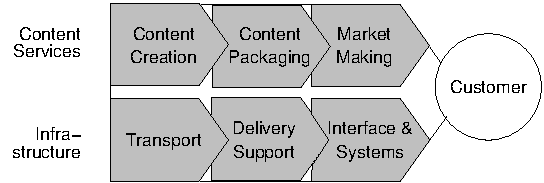
\includegraphics[width=\textwidth]{images/indica_model.pdf}
    \caption{The INDICA two-layered value chain model.}
    \label{fig:indica_model}
  \end{center}
\end{figure}

You can also include JPEG or PNG files, as shown by Figure~\ref{fig:eeyore}.

\begin{figure}[ht]
  \begin{center}
    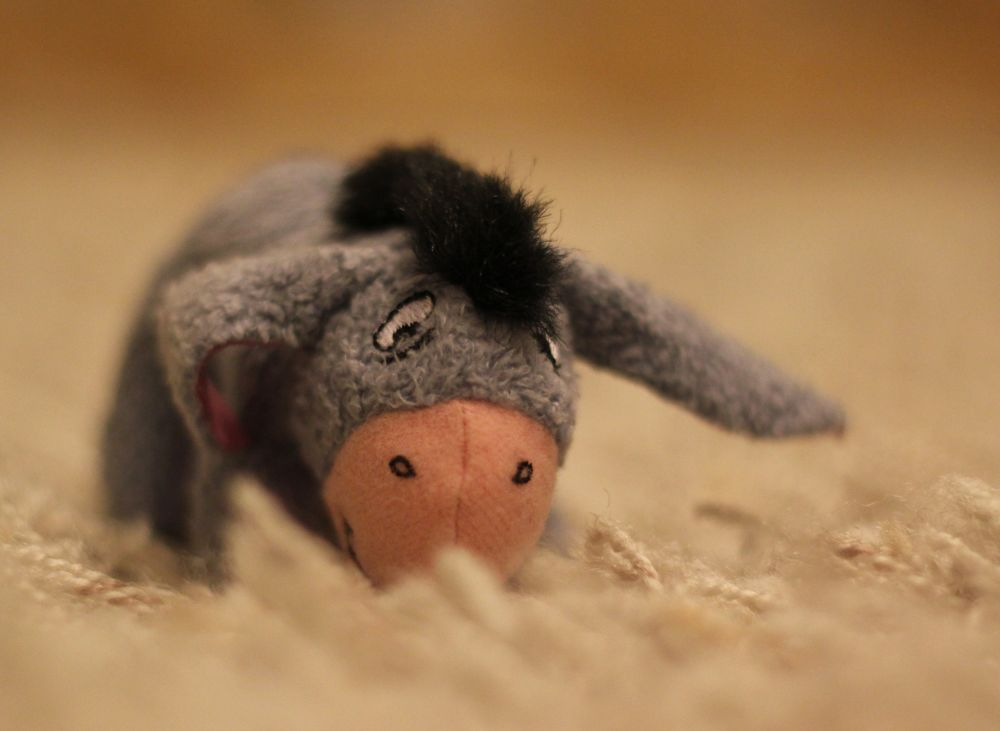
\includegraphics[width=9cm]{images/ihaa.jpg}
    \caption{Eeyore, or Ihaa, a very sad donkey.}
    \label{fig:eeyore}
  \end{center}
\end{figure}

You can create PDF files out of practically anything. 
In Windows, you can download PrimoPDF or CutePDF (or some such) and install a
printing driver so that you can print directly to PDF files from any
application. There are also tools that allow you to upload documents in common
file formats and convert them to the PDF format.
If you have PS or EPS files, you can use the tools \texttt{ps2pdf} or
\texttt{epspdf} to convert your PS and EPS files to PDF\@.

% Comment: If your sentence ends in a capital letter, like here, you should
% write \@ before the period; otherwise LaTeX will assume that this is not
% really an end of the sentence and will not put a large enough space after the
% period. That is, LaTeX assumes that you are (for example), enumerating using
% capital roman numerals, like I. do something, II. do something else. In this
% case, the periods do not end the sentence.

% Similarly, if you do need a normal space after a period (instead of
% the longer sentence separator), use \  (backslash and space) after the
% period. Like so: a.\ first item, b.\ second item.

Furthermore, most newer editor programs allow you to save directly to the PDF
format. For vector editing, you could try Inkscape, which is a new open source
WYSIWYG vector editor that allows you to save directly to PDF\@. 
For graphs, either export/print your graphs from OpenOffice Calc/Microsoft
Excel to PDF format, and then add them; or use \texttt{gnuplot}, which can
create PDF files directly (at least the new versions can).
The terminal type is \emph{pdf}, so the first line of your plot file should be
something like \texttt{set term pdf \ldots}.

To get the most professional-looking graphics, you can encode them using the
TikZ package (TikZ is a frontend for the PGF graphics formatting system).
You can create practically any kind of technical images with TikZ, but it has a
rather steep learning curve. Locate the manual (\texttt{pgfmanual.pdf}) from
your \LaTeX\ distribution and check it out. An example of TikZ-generated
graphics is shown in Figure~\ref{fig:page-merge}.

\begin{figure}[ht]
  \begin{center}
    \newcommand*{\actver}{\smash{\ensuremath{v_{\text{\textit{active}}}}}}

\tikzstyle{lbl}=[font=\scriptsize,midway,sloped]
\tikzstyle{opendash}=[densely dotted,thick] 
\tikzstyle{opendeco}=[decoration={zigzag,amplitude=0.1em,segment length=0.6em}]
\tikzstyle{actverline}=[dashed]
\tikzstyle{entryline}=[densely dotted]
\tikzstyle{area}=[ellipse,draw,dashed]
\tikzstyle{liveentry}=[entryline,postaction={%
  decorate,%
  decoration={%
    markings,%
    mark=at position .5pt with{\arrowreversed[line width=.35pt]{|}};,
    mark=at position 1 with{%
      \arrow[line width=.8pt]{stealth}};%
  }%
}]
\tikzstyle{deadentry}=[entryline,postaction={%
  decorate,%
  decoration={%
    markings,%
    mark=at position .5pt with{\arrowreversed[line width=.35pt]{|}};,
    mark=at position 1 with{%
      \arrow[line width=.8pt]{stealth}};%
%      \arrow[line width=.35pt,black,fill=white]{*}};% 
  }%
}]
\tikzstyle{pageborder}=[thick]
\tikzstyle{pagename}=[anchor=center,text=black!50,font=\huge]
\newlength{\spexx}
\setlength{\spexx}{1.2cm}
\newlength{\spexy}
\setlength{\spexy}{.5cm}

\subfigure[Before]{
\begin{tikzpicture}[x=\spexx,y=\spexy,%
  every pin edge/.style={draw,dotted},%
  pin distance=.5\spexx]
  \small
  \coordinate (lo) at (0,-5);
  \coordinate (o) at (0,0);
  \coordinate (hi) at (0,7);
  \coordinate (loact) at (3,-5);
  \coordinate (oact) at (3,0);
  \coordinate (hiact) at (3,7);
  \coordinate (loinf) at (4,-5);
  \coordinate (oinf) at (4,0);
  \coordinate (hiinf) at (4,7);
  
  \draw[->] (lo) -- node[below,lbl] {Versions} ($(loinf) + (1em,0)$);
  \draw[->] (lo) -- node[above,lbl] {Keys} ($(hi) + (0,1em)$);

  \draw[pageborder] (lo) -- (o) -- (hi);
  \draw[pageborder] (lo) -- (loinf);
  \draw[pageborder] (hi) -- (hiinf);
  \draw[pageborder] (o) -- (oinf);

  \draw[opendash] decorate [opendeco] { (loinf) -- (oinf) };
  \draw[opendash] decorate [opendeco] { (oinf) -- (hiinf) };

  \node[pagename] at (2,3.5) {$p$};
  \node[pagename] at (2,-2.5) {$s$};

  \draw[actverline] ($(loact) + (0,-1em)$) node[below=.4em] {\actver} --
    ($(hiact) + (0,1em)$);

  % Page p contents
  \draw[deadentry] (0,6) -- (1,6);
  \draw[deadentry] (1,6) -- (2,6);
  \draw[deadentry] (2,6) -- (3,6);
  \draw[liveentry] (0,5) -- (4,5);
  \draw[deadentry] (0,4) -- (2,4);
  \draw[deadentry] (1,3) -- (3,3);
  \draw[deadentry] (0,2) -- (1,2);
  \draw[deadentry] (2,2) -- (3,2);
  \draw[deadentry] (0,1) -- (2,1);
  \draw[deadentry] (2,1) -- (3,1);

  % Page s contents
  \draw[liveentry] (0,-1) -- (4,-1);
  \draw[deadentry] (0,-2) -- (2,-2);
  \draw[deadentry] (0,-3) -- (3,-3);
  \draw[liveentry] (3,-4) -- (4,-4);

  \node[area,minimum width=4.5\spexx,minimum height=.6\spexy,pin=178:{$1$}]
    at (2,5) {};
  \node[area,minimum width=4.5\spexx,minimum height=.6\spexy,pin=182:{$2$}]
    at (2,-1) {};
  \node[area,minimum width=1.5\spexx,minimum height=.6\spexy,pin=330:{$3$}]
    at (3.5,-4) {};

\end{tikzpicture}}
\subfigure[After]{
\begin{tikzpicture}[x=\spexx,y=\spexy,%
  every pin edge/.style={draw,dotted},%
  pin distance=.5\spexx]
  \small
  \coordinate (lo) at (0,-5);
  \coordinate (o) at (0,0);
  \coordinate (hi) at (0,7);
  \coordinate (loact) at (3,-5);
  \coordinate (oact) at (3,0);
  \coordinate (hiact) at (3,7);
  \coordinate (loinf) at (4,-5);
  \coordinate (oinf) at (4,0);
  \coordinate (hiinf) at (4,7);

  \draw[->] (lo) -- node[lbl,below] {Versions} ($(loinf) + (1em,0)$);
  \draw[->] (lo) -- node[lbl,above] {Keys} ($(hi) + (0,1em)$);

  \draw[pageborder] (lo) -- (o) -- (hi);
  \draw[pageborder] (lo) -- (loinf);
  \draw[pageborder] (hi) -- (hiinf);
  \draw[pageborder] (o) -- (oact);

  \draw[opendash] decorate [opendeco] { (loinf) -- (oinf) };
  \draw[opendash] decorate [opendeco] { (oinf) -- (hiinf) };

  \node[pagename] at (1.5,3.5) {$p$};
  \node[pagename] at (1.5,-2.5) {$s$};
  \node[pagename] at (3.5,1) {$p'$};

  \draw[actverline] ($(loact) + (0,-1em)$) node[below=.4em] {\actver} -- (loact);
  \draw[pageborder] (loact) -- (hiact);
  \draw[actverline] (hiact) -- ($(hiact) + (0,1em)$);

  % Page p contents
  \draw[deadentry] (0,6) -- (1,6);
  \draw[deadentry] (1,6) -- (2,6);
  \draw[deadentry] (2,6) -- (3,6);
  \draw[deadentry] (0,5) -- (3,5);
  \draw[deadentry] (0,4) -- (2,4);
  \draw[deadentry] (1,3) -- (3,3);
  \draw[deadentry] (0,2) -- (1,2);
  \draw[deadentry] (2,2) -- (3,2);
  \draw[deadentry] (0,1) -- (2,1);
  \draw[deadentry] (2,1) -- (3,1);

  % Page s contents
  \draw[deadentry] (0,-1) -- (3,-1);
  \draw[deadentry] (0,-2) -- (2,-2);
  \draw[deadentry] (0,-3) -- (3,-3);

  % Page p' contents
  \draw[liveentry] (3,5) -- (4,5);
  \draw[liveentry] (3,-1) -- (4,-1);
  \draw[liveentry] (3,-4) -- (4,-4);

  \node[area,minimum width=1.5\spexx,minimum height=.6\spexy,pin=10:{$1$}]
    at (3.5,5) {};
  \node[area,minimum width=1.5\spexx,minimum height=.6\spexy,pin=3:{$2$}]
    at (3.5,-1) {};
  \node[area,minimum width=1.5\spexx,minimum height=.6\spexy,pin=330:{$3$}]
    at (3.5,-4) {};
\end{tikzpicture}}

    \caption{Example of a multiversion database page merge. This figure has
    been taken from the PhD thesis of Haapasalo~\cite{HaapasaloThesis}.}
    \label{fig:page-merge}
  \end{center}
\end{figure}

Another example of graphics created with TikZ is shown in
Figure~\ref{fig:tikz-examples}. 
These show how graphs can be drawn and labeled. 
You can consult the example images and the PGF manual for more examples of what
kinds figures you can draw with TikZ. 

% These definitions are only used in the example images; you will not 
% need them for your thesis...
\newlength{\graphdotsize}
\setlength{\graphdotsize}{1.7pt}
\newlength{\graphgridsize}
\setlength{\graphgridsize}{1.2em}
\begin{figure}[ht]
\begin{center}
\subfigure[Examples of obstruction graphs for the Ferry Problem]{
  \newlength{\oggs}
\setlength{\oggs}{1.2\graphgridsize}
\begin{tikzpicture}[x=\oggs,y=\oggs,every pin edge/.style={draw,dotted},pin distance=0.5\oggs,area/.style={ellipse,draw,dashed}] 

% The graph (0,0,5,0)
% o = origo
\coordinate (o) at (0,0);
\coordinate[left=1 of o,pin=100:$q_1$] (q1);
\coordinate[right=1 of o,pin=80:$q_2$] (q2);
\fill[black] (q1) circle (\graphdotsize);
\fill[black] (q2) circle (\graphdotsize);
\foreach \d in {-2, -1, ..., 2} {
  \coordinate (tmp) at ($(o) + (0,\d)$);
  \draw (q1) -- (tmp);
  \draw (q2) -- (tmp);
  \fill[black] (tmp) circle (\graphdotsize);
}
\node[area,minimum height=5.3\oggs,minimum width=0.8\oggs,pin=94:$X_3$] at (o) {};  

% The graph (1,0,3,0)
\coordinate[right=5 of o] (o);
\coordinate[left=1 of o,pin=260:$q_1$] (q1);
\coordinate[left=2 of o] (q1v);
\coordinate[right=1 of o,pin=280:$q_2$] (q2);
\fill[black] (q1) circle (\graphdotsize);
\fill[black] (q2) circle (\graphdotsize);
\fill[black] (q1v) circle (\graphdotsize);
\draw (q1) -- (q1v);
\foreach \d in {-1, 0, 1} {
  \coordinate (tmp) at ($(o) + (0,\d)$);
  \draw (q1) -- (tmp);
  \draw (q2) -- (tmp);
  \fill[black] (tmp) circle (\graphdotsize);
}
\node[area,minimum height=3.3\oggs,minimum width=0.8\oggs,pin=266:$X_3$] at (o) {};  
\node[area,minimum height=0.8\oggs,minimum width=0.8\oggs,pin=260:$X_1$] at (q1v) {};  


% The graph (0,1,3,0)
\coordinate[right=4 of o] (o);
\coordinate[left=1 of o,pin=100:$q_1$] (q1);
\coordinate[right=1 of o,pin=80:$q_2$] (q2);
\coordinate[right=2 of o] (q2v);
\fill[black] (q1) circle (\graphdotsize);
\fill[black] (q2) circle (\graphdotsize);
\fill[black] (q2v) circle (\graphdotsize);
\draw (q2) -- (q2v);
\foreach \d in {-1, 0, 1} {
  \coordinate (tmp) at ($(o) + (0,\d)$);
  \draw (q1) -- (tmp);
  \draw (q2) -- (tmp);
  \fill[black] (tmp) circle (\graphdotsize);
}
\node[area,minimum height=3.3\oggs,minimum width=0.8\oggs,pin=94:$X_3$] at (o) {};  
\node[area,minimum height=0.8\oggs,minimum width=0.8\oggs,pin=80:$X_2$] at (q2v) {};  

% The graph (0,0,3,1)
\coordinate[right=5 of o] (o);
\coordinate[left=1 of o,pin=260:$q_1$] (q1);
\coordinate[right=1 of o,pin=290:$q_2$] (q2);
\fill[black] (q1) circle (\graphdotsize);
\fill[black] (q2) circle (\graphdotsize);
\draw (q1) -- (q2);
\foreach \d in {-1, 1, 2} {
  \coordinate (tmp) at ($(o) + (0,\d)$);
  \draw (q1) -- (tmp);
  \draw (q2) -- (tmp);
  \fill[black] (tmp) circle (\graphdotsize);
}
\node[area,minimum height=4.3\oggs,minimum width=0.8\oggs,pin=266:$X_3$] at ($(o) + (0,0.5)$) {};  

\end{tikzpicture}

}
\subfigure[Examples of star graphs]{
  \begin{tikzpicture}[x=\graphgridsize,y=\graphgridsize] 

\coordinate (o) at (0,0);
\fill[black] (o) circle (\graphdotsize);
\foreach \d in {0, 90, ..., 270} {
  \coordinate (tmp) at ($(o) + (\d:1.5)$);
  \draw (o) -- (tmp);
  \fill[black] (tmp) circle (\graphdotsize);
}

\coordinate[right=4 of o] (o);
\coordinate (o1) at ($(o) + (0:0.3)$);
\coordinate (o2) at ($(o) + (180:0.3)$);
\fill[black] (o1) circle (\graphdotsize);
\fill[black] (o2) circle (\graphdotsize);
\draw (o1) -- (o2);
\foreach \d in {45, 135, 270} {
  \coordinate (tmp\d) at ($(o) + (\d:1.5)$);
  \draw (o2) -- (tmp\d);
  \fill[black] (tmp\d) circle (\graphdotsize);
}
\draw (o1) -- (tmp45);


\coordinate[right=4 of o] (o);
\coordinate (o1) at ($(o) + (0:0.3)$);
\coordinate (o2) at ($(o) + (180:0.3)$);
\fill[black] (o1) circle (\graphdotsize);
\fill[black] (o2) circle (\graphdotsize);
\draw (o1) -- (o2);
\foreach \d in {45, 135, 270} {
  \coordinate (tmp\d) at ($(o) + (\d:1.5)$);
  \draw (o2) -- (tmp\d);
  \fill[black] (tmp\d) circle (\graphdotsize);
}
\draw (o1) -- (tmp45);
\draw (o1) -- (tmp135);


\coordinate[right=4 of o] (o);
\coordinate (o1) at ($(o) + (0:0.3)$);
\coordinate (o2) at ($(o) + (180:0.3)$);
\fill[black] (o1) circle (\graphdotsize);
\fill[black] (o2) circle (\graphdotsize);
\draw (o1) -- (o2);
\foreach \d in {45, 135, 270} {
  \coordinate (tmp\d) at ($(o) + (\d:1.5)$);
  \draw (o1) -- (tmp\d);
  \draw (o2) -- (tmp\d);
  \fill[black] (tmp\d) circle (\graphdotsize);
}


\coordinate[right=3.5 of o] (o);
\coordinate (o1) at ($(o) + (90:0.3)$);
\coordinate (o2) at ($(o) + (210:0.5)$);
\coordinate (o3) at ($(o) + (330:0.5)$);
\fill[black] (o1) circle (\graphdotsize);
\fill[black] (o2) circle (\graphdotsize);
\fill[black] (o3) circle (\graphdotsize);
\draw (o1) -- (o2);
\draw (o1) -- (o3);
\draw (o2) -- (o3);
\foreach \d in {90, 270} {
  \coordinate (tmp\d) at ($(o) + (\d:1.5)$);
  \draw (o2) -- (tmp\d);
  \draw (o3) -- (tmp\d);
  \fill[black] (tmp\d) circle (\graphdotsize);
}
\draw (o1) -- (tmp90);


\coordinate[right=3 of o] (o);
\coordinate (o1) at ($(o) + (90:0.3)$);
\coordinate (o2) at ($(o) + (210:0.5)$);
\coordinate (o3) at ($(o) + (330:0.5)$);
\fill[black] (o1) circle (\graphdotsize);
\fill[black] (o2) circle (\graphdotsize);
\fill[black] (o3) circle (\graphdotsize);
\draw (o1) -- (o2);
\draw (o1) -- (o3);
\draw (o2) -- (o3);
\foreach \d in {90, 270} {
  \coordinate (tmp\d) at ($(o) + (\d:1.5)$);
  \draw (o2) -- (tmp\d);
  \draw (o3) -- (tmp\d);
  \fill[black] (tmp\d) circle (\graphdotsize);
}
\draw (o1) -- (tmp90);
\draw (o1) -- (tmp270);



\coordinate[right=3.5 of o] (o);
\coordinate (o1) at ($(o) + (18:1.3)$);
\coordinate (o2) at ($(o) + (90:1.3)$);
\coordinate (o3) at ($(o) + (162:1.3)$);
\coordinate (o4) at ($(o) + (234:1.3)$);
\coordinate (o5) at ($(o) + (306:1.3)$);
\foreach \d in {1, 2, ..., 5} {
  \fill[black] (o\d) circle (\graphdotsize);
}
\draw (o1) -- (o2);
\draw (o1) -- (o3);
\draw (o1) -- (o4);
\draw (o1) -- (o5);
\draw (o2) -- (o3);
\draw (o2) -- (o4);
\draw (o2) -- (o5);
\draw (o3) -- (o4);
\draw (o3) -- (o5);
\draw (o4) -- (o5);

\end{tikzpicture}

}
\caption{Examples of graphs draw with TikZ. These figures have been taken from a
course report for the graph theory course~\cite{FerryProblem}.}
\label{fig:tikz-examples}
\end{center}
\end{figure}



\chapter{Software process improvement maturity models}
\chaptermark{maturity models}
\label{chapter:maturitymodels}

According to O'Regan \citep{RefWorks:29} the software process improvement is "a program of activities designed to improve the performance and maturity of the organization's software processes and the results of such a program." In practice, the aim of SPI is to meet the business goals more efficiently and to improve the software quality. In other words, it aims for smarter work and better software, in less time. Many process models or frameworks are created for the software process improvement and one of them, the Capability Maturity Model Integration (CMMI), is presented in this chapter. Because of the usability approach of this thesis, a model emphasizing the human-centeredness is also discussed. The user-centered process model for SPI is called Usability Maturity Model (UMM). \citep{RefWorks:29}

\section{Capability Maturity Model Integration}
The Capability Maturity Model Integration was developed in the early 1990s by the Software Engineering Institute. The purpose of the institute is to define best practices for software processes and thereby improve their maturity. The object of interest in this Master's thesis is the development version of the model, called CMMI for Development (CMMI-DEV). It provides a carefully defined road map and  structured approach for the software process improvement, and allows companies to set their own improvement goals and priorities. The CMMI consist of five maturity levels and each level includes a number of process areas. These process areas consist of a set of goals which needs to be implemented by the defined practices. The practices specify the actual actions to be accomplished. A maturity level is achieved when all the process areas of that maturity level have been implemented. \citep{RefWorks:29}

Once the CMMI is initialized (at the first level), the level two focuses on project management practices such as requirement management and project planning. The third level of the model requires the implementation of engineering procedures and standards. For example, design, coding and testing procedures should be defined throughly for effective risk management and decision analysis. The requirement of the fourth CMMI level is that the process performance is achieved within the defined limits set by the company. The implementation of the level also requires the usage of quantitative metrics and goals to be set for the performance. The last level of the model requires a culture of continuous improvement in the company. The possible defects need to be identified and actions to be taken to prevent them from re-occurring. Each of the levels and their improvements forms the basis of the next level in the Capability Majority Model. \citep{RefWorks:29}

The level representation of the CMMI is described in Figure \ref{fig:cmmi} including the levels and the CMMI process areas. Every process area consists of \textbf{specific} and \textbf{generic} goals and practices. The specific goals and practices are unique for each process area, and describes what needs to be accomplished to perform the process. The specific practices which are connected to the specific goals describe the activities to achieve the goals. However, the generic goals and practices are common for all the process areas in the CMMI level. The implementation of the generic practices institutionalizes the process, meaning that the process is documented, defined and understood, and that the process users are appropriately trained. The generic goals can be used, for example, to manage, define, and optimize the organization processes.\citep{RefWorks:29}	

\begin{figure}[H]
  	\centering
  	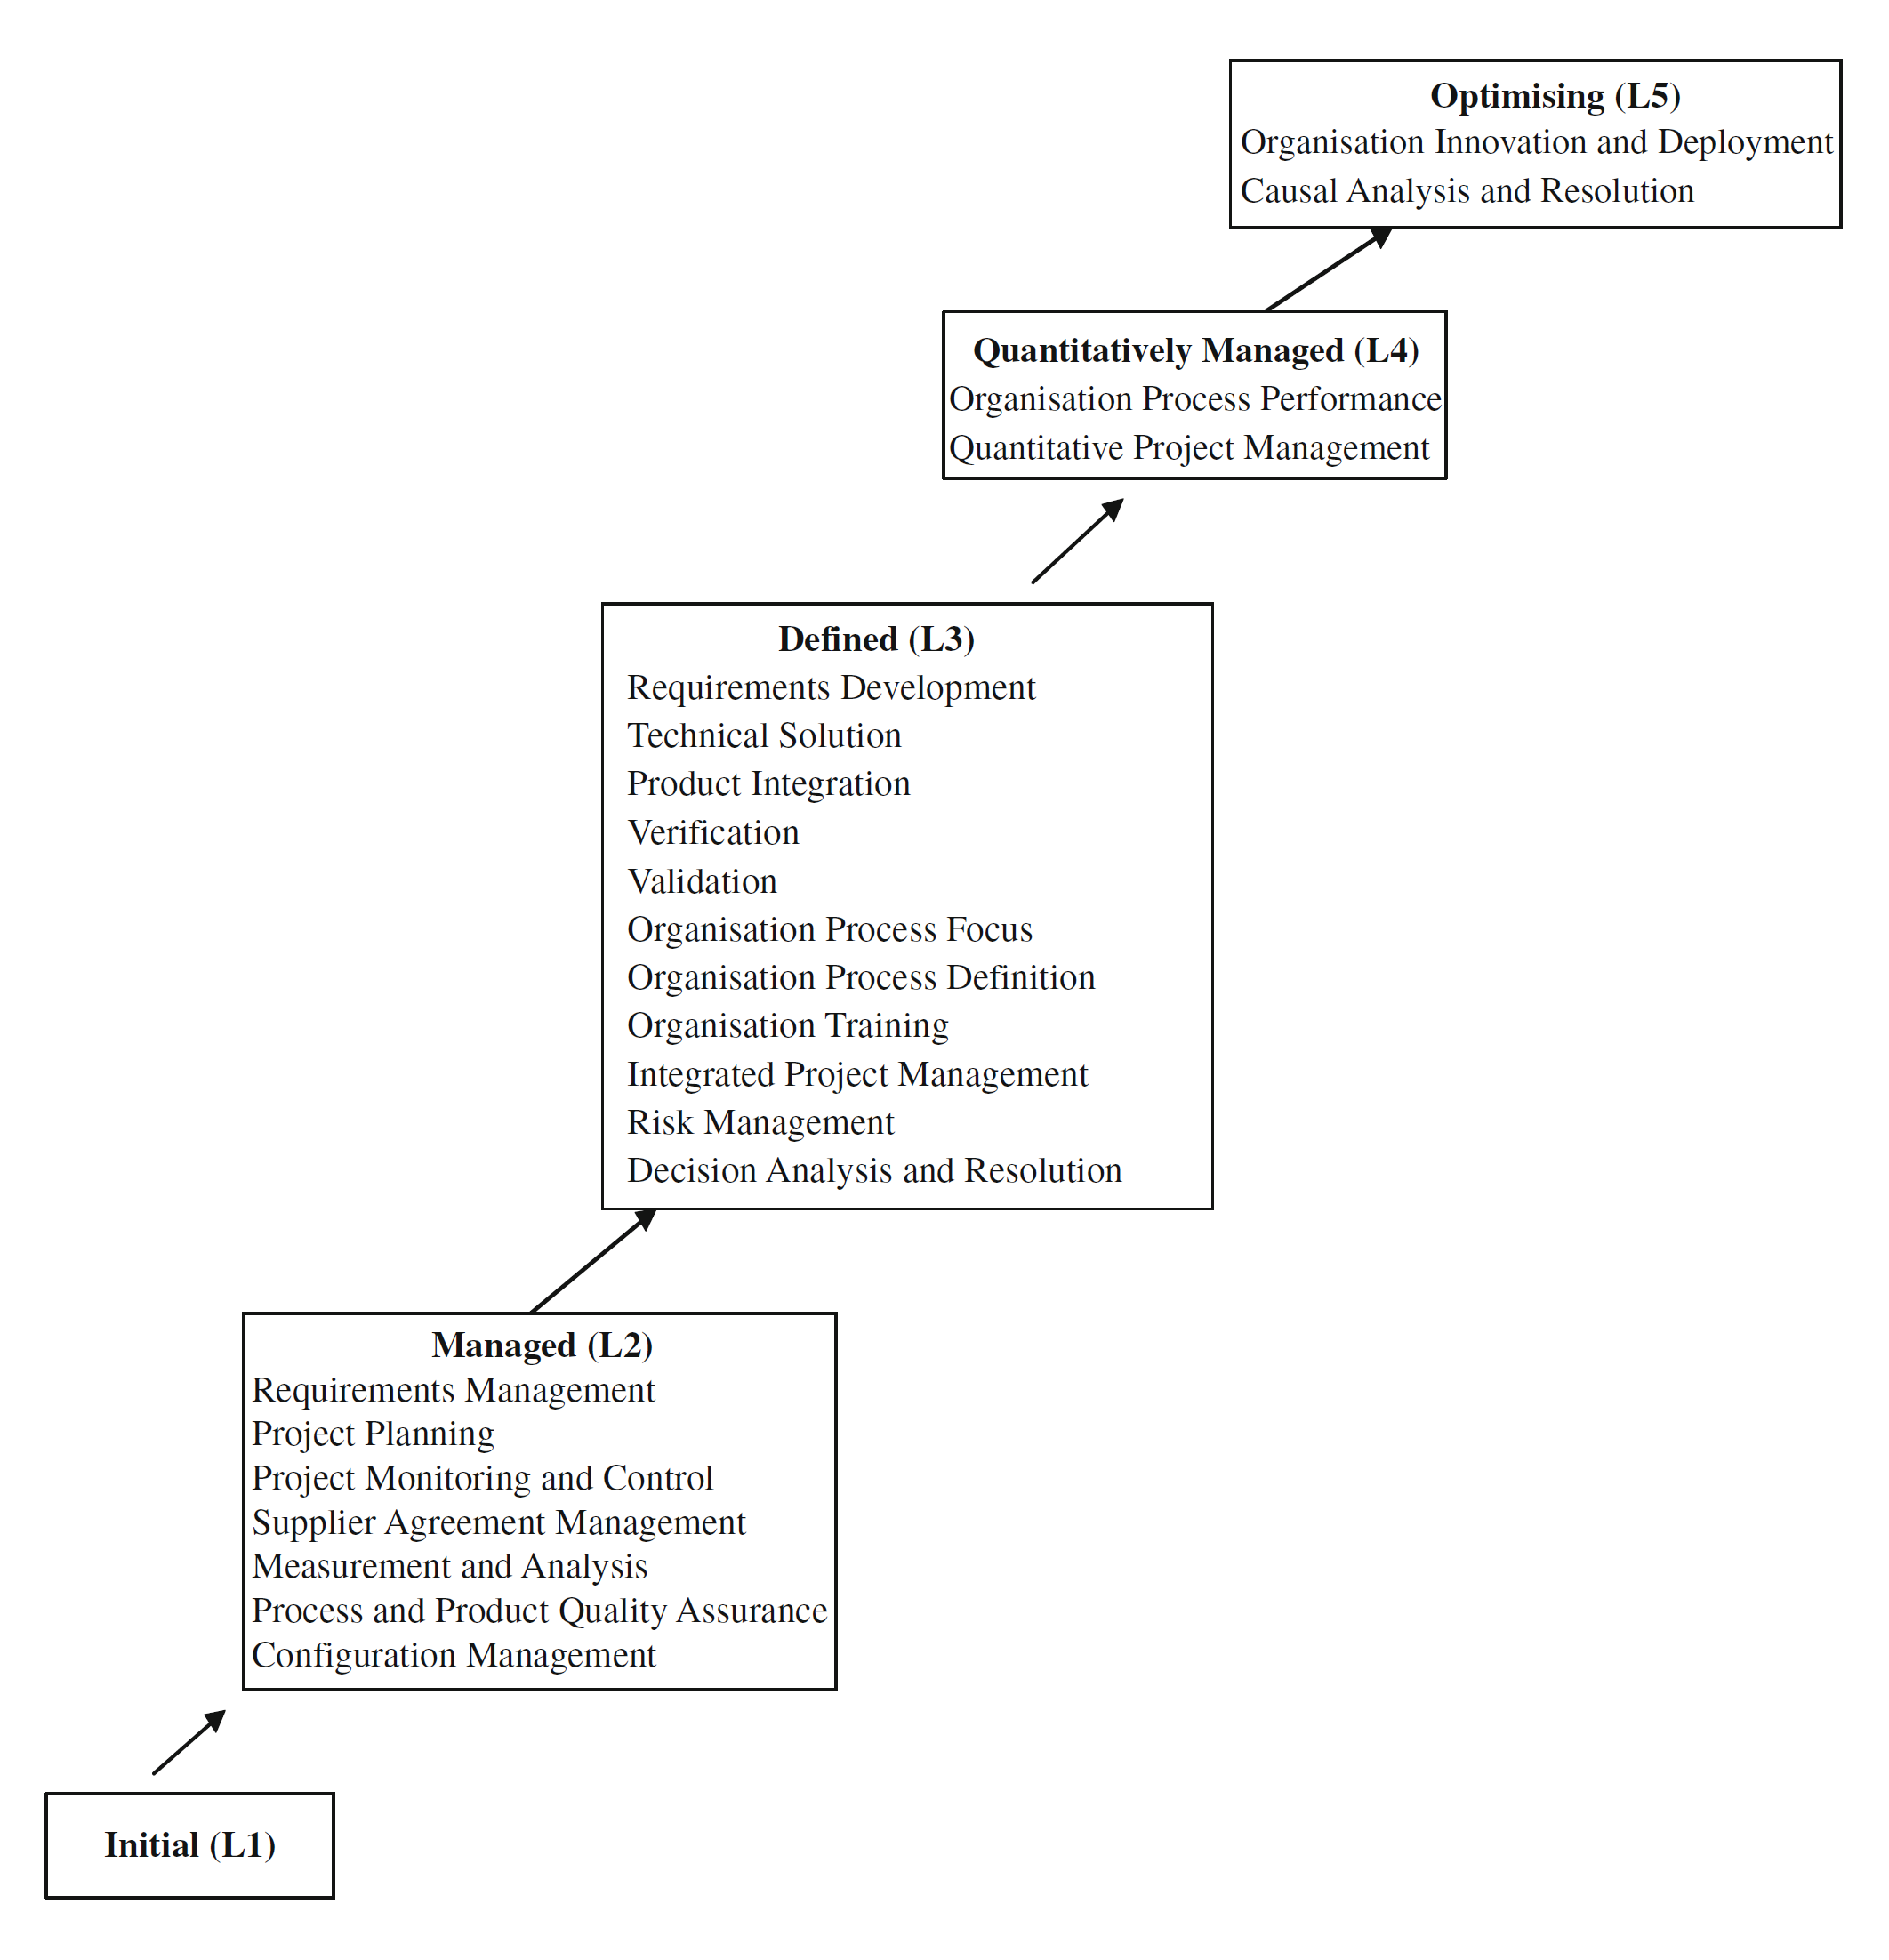
\includegraphics[width=0.9\textwidth]{./images/cmmi_levels.png}
  	\caption{Capability Maturity Model Integration: Maturity levels. \citep{RefWorks:29}}
	\label{fig:cmmi}
\end{figure}



\section{Usability Maturity Model}
The Capability Maturity Model Integration is a good example of a model for software process improvement, but it doesn't consider the human-centered part of system development. The Usability Maturity Model has been created as a scale to measure the human-centeredness of system development projects. In other words, UMM is a method to evaluate organization's capability to implement human-centered design. It has many corresponding elements with other SPI models, such as ISO TR 15504 standard, but it is still considered a stand-alone model. \citep{RefWorks:30}	

 \subsection{Maturity levels of the model}
Like CMMI, also the Usability Maturity Model consists of maturity levels (see Figure \ref{fig:umm}).The UMM consist of six maturity levels and the first one is called level X, in which the need for human-centered activities is not recognized at all. At the level A, the organization has recognized the need for improving systems quality of use. The next improvement, level A1, is a problem recognition attribute and describes the extent of problem internalization. To achieve level A1 maturity, the staff and the management need to be aware of the need for improvements. Level A2 describes a number of processes to be performed, which then provide an input for human-centered activities. Additionally, practices should be performed in order to gather user requirements, which then should be included in the usability information collection. In level B, the organization indicates to the staff that the quality of use is considered as an important asset in the development, and trains the staff to be aware that the usability can be improved by considering the user requirements. The level B1 can be achieved by training the human-centered methods and human-system interaction principles. The employees need to focus on the users by trying, for instance, to understand the end users' skills, backgrounds and motivations (Level B2). \citep{RefWorks:30}

The human-centered processes are already implemented in the level C. Users are involved in system specification and process testing, and the suitable human-centered techniques are being employed. An active participation of the users, the creation of UX, the user defined quality of use, continuous testing, and feedback, are required in order for the organization to achieve the C1 maturity level. On the other hand, the level C2 requires the use of appropriate usability methods, suitable facilities and tools, as well as usability technique maintenance. The last requirement includes reviewing the suitability of the methods and the usage of state-of-the-art UI technologies. The level C3 can be achieved by ensuring the defined and required human-centered competences of the employees. In level D, and in all the sub-levels, the human-centered processes are integrated to the system's life cycle and quality processes. What is more, the necessary time and resources are targeted for these activities, the interaction with other departments is successful, feedback process is properly administered, and the design solutions are being iterated. \citep{RefWorks:30}

The last UMM level is level E and its sub-levels. They require the institutionalization of the human-centered processes, which means that the organization gains benefit from its human-centeredness. On this maturity level, usability skills and engineering skills are used together, and the usability defects are managed in a similar manner to other system defects. In addition, human-centered process is being included in the projects, and thereby the usability is systematically improved. Generally speaking, human-centredness has an influence to the whole organization. \citep{RefWorks:30}

\begin{figure}[H]
  	\centering
  	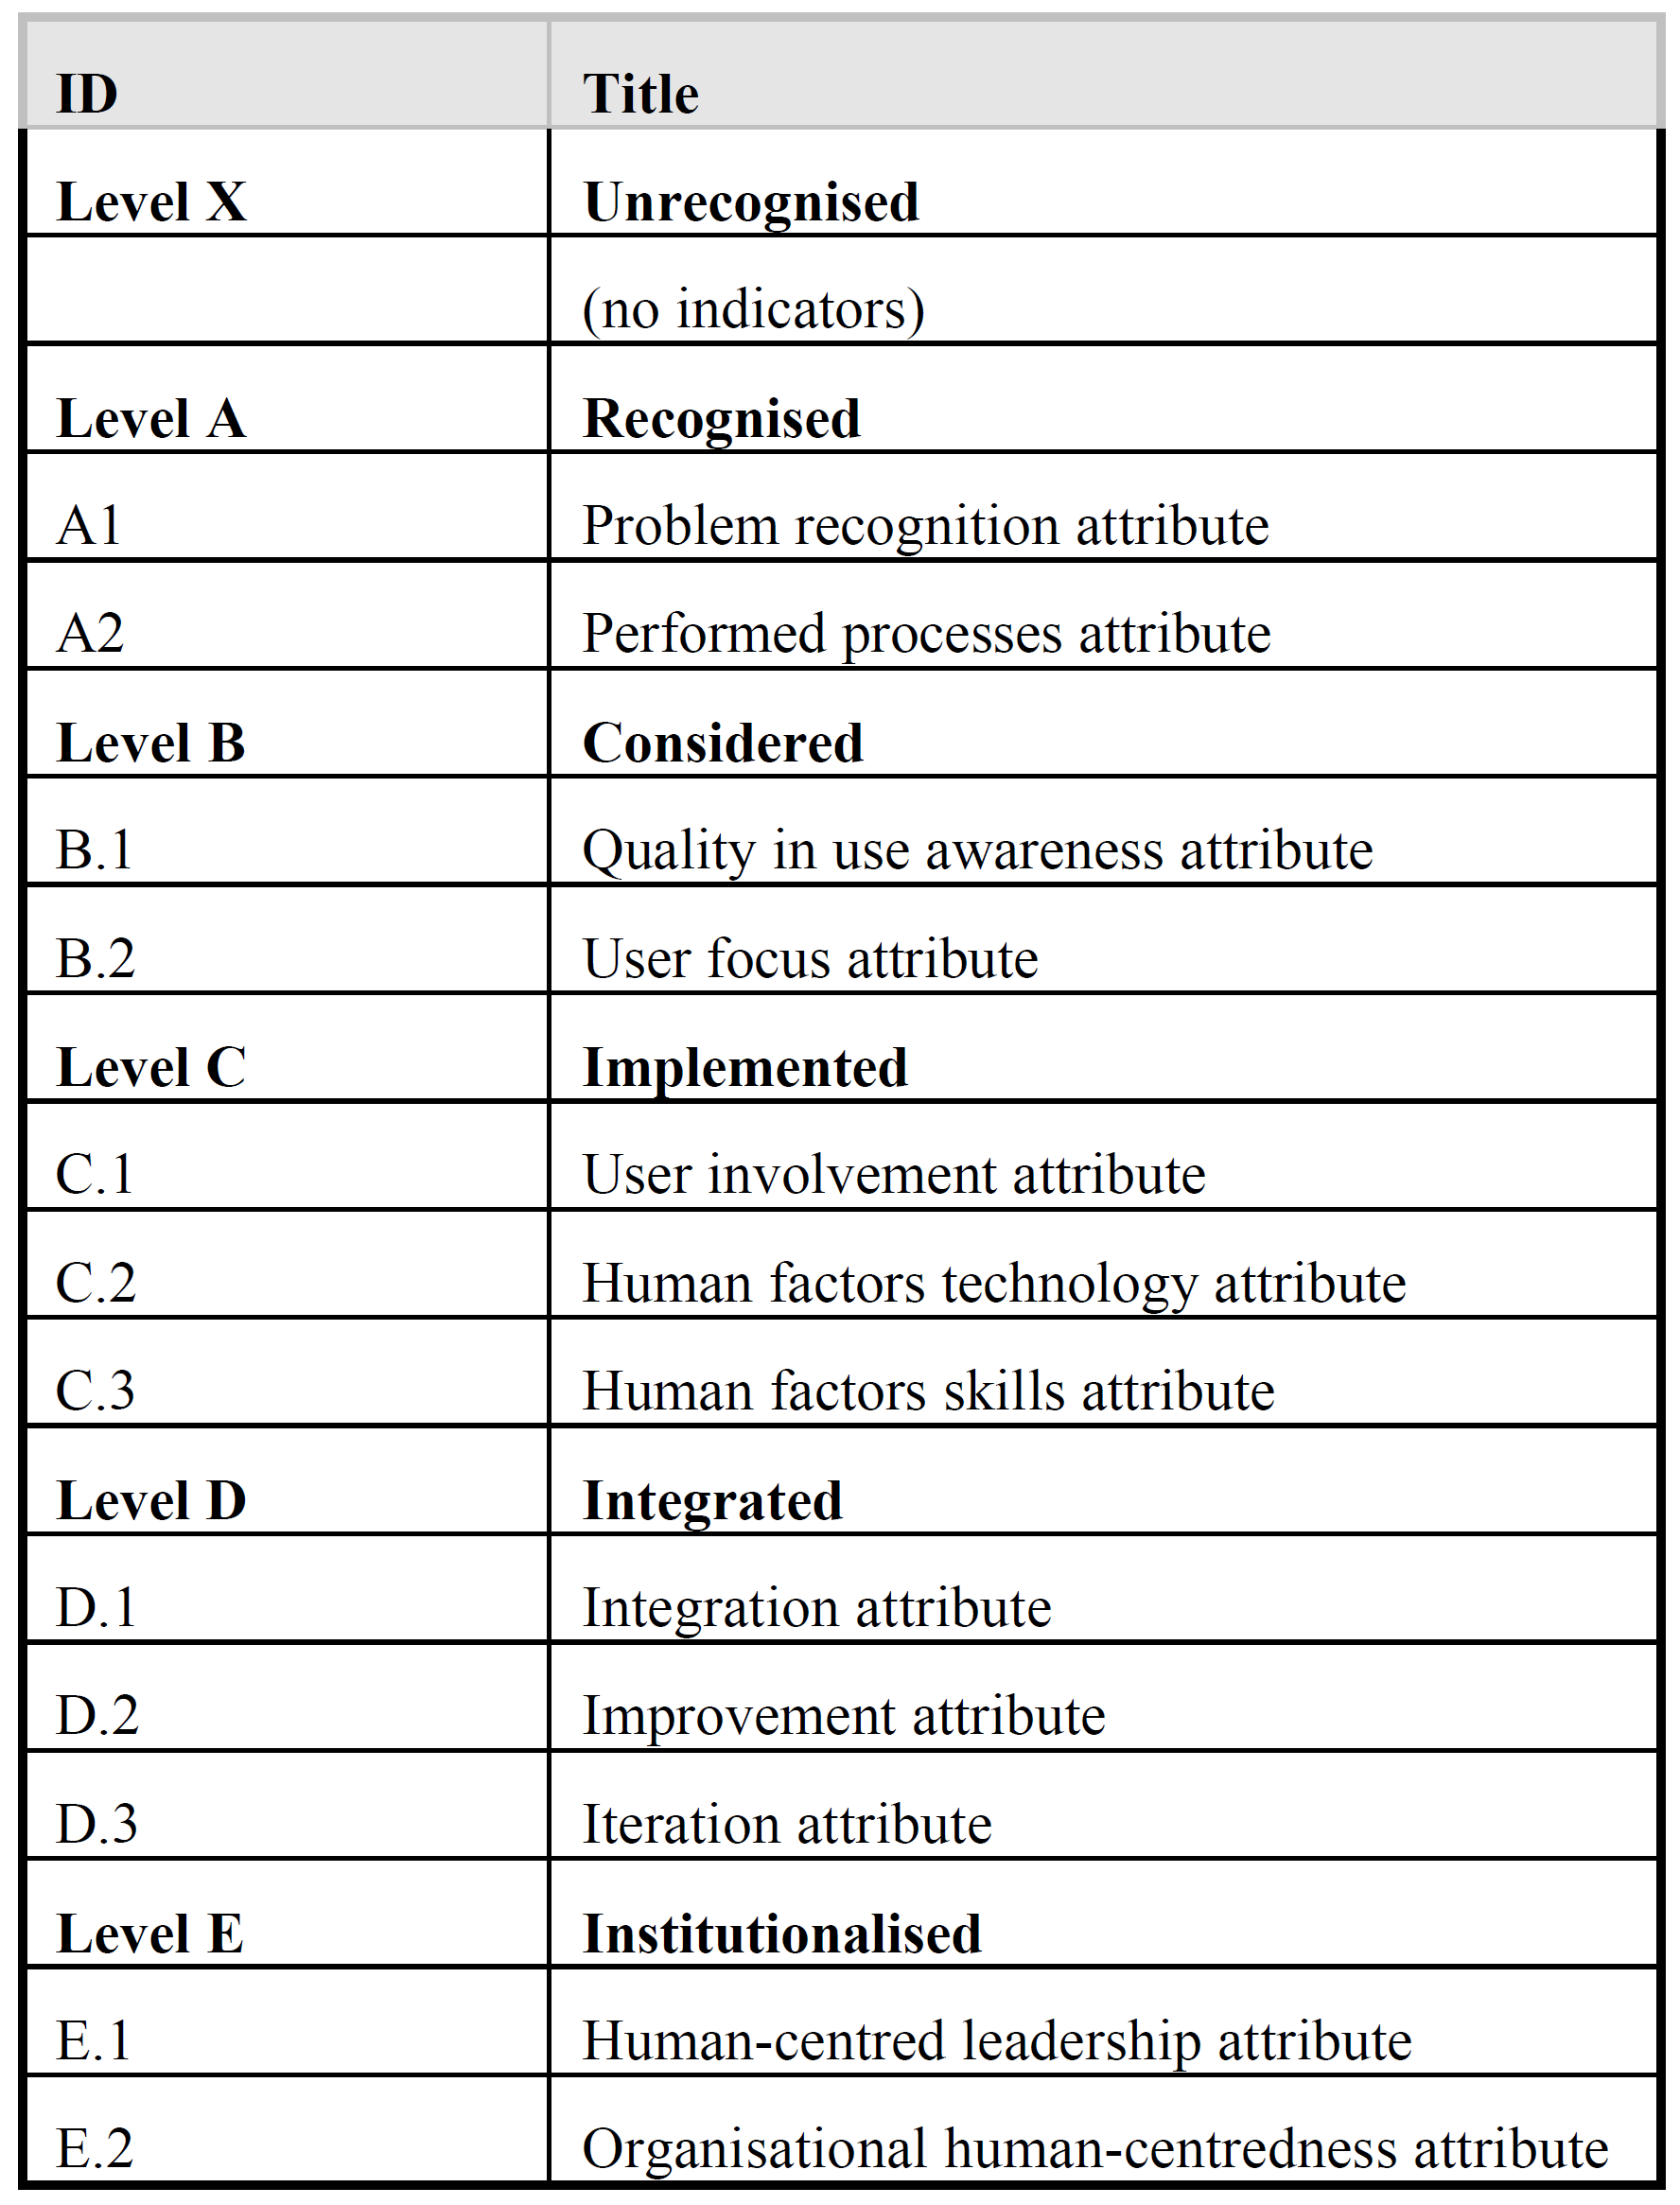
\includegraphics[width=0.7\textwidth]{./images/umm_levels.png}\hspace*{4cm}
  	\caption{Usability Maturity Model: Maturity levels and process attributes. \citep{RefWorks:30}}
	\label{fig:umm}
\end{figure}

\subsection{Level transitions}

The transitions between the maturity levels change the organization and the changes create the basis for software process improvement. In the case of UMM, the transitions represent improvements in the usability consciousness. 

The transition between maturity levels A and B is a cultural change, from experience based, to more user-centric engineering. In level A, the attitude against user-centeredness might be incredulous, but in level B the awareness of the system being used by the people, has been created. The transition from level B to C creates the cultural change of user being considered throughout the development process. Additionally, the differences between analyst and end-users are being recognized. \citep{RefWorks:30}

The change from the level of considering the users, to the implementation of the human-centered processes (from level C to D) requires the routine use of human factors expertise, and human-centered methods and tools. The user involving the development process is considered as a normal procedure at the level D. The transition from the level D to level E institutionalizes the human-centeredness. The system development is then embedded in a business-driven culture, which changes the focus (of the development) from the functionality of the supporting systems to what the organization is able to do in general. In other words, the system functionality is not the core issue any longer.  \citep{RefWorks:30}

\subsection{Model application}

The organization needs to delegate one person to be in charge of the quality of use. The first task of the employee is to examine the awareness of the human-centered principles within the organization, by interviewing the managerial level. This information can be used to assess the maturity level of the organization. However, more than one project should be assessed in order to gain wider understanding and proof about the current maturity level. The performance assessment forms the basis for reviews and improvements of the human-centered processes in the organization. \citep{RefWorks:30}

\chapter{Methods for user-centered software process improvement}
\chaptermark{Methods}
\label{chapter:methods}


In order to be able to discover reliable research data, the research methods must be understood thoroughly. This study gathers data by utilizing a few types of usability methods which are selected according to their practicality and utility for the study context. In general, the methods used in this research study can be used as a part of human-centered design process. The reasoning for the choice of the methods is defined in more detail in section \ref{sec:dprocess}. 


\section{Remote usability logging}
\label{sec:rue}

There are multiple ways to implement a remote usability evaluation. Typically, it is implemented by sending surveys or asking for feedback after the system deployment. This kind of information is an important indicator of the user satisfaction, but does not give any specific details about the usage of the system. However, the usage data is essential to isolate the problems in usability. One approach to access the data remotely, is to use data logging method. In the context of usability evaluation, data logging stands for mechanical practices to record the usage of a system. \citep{RefWorks:31}

Usage data may offer valuable information about users' actions and can thus be utilized in the process of improving software's usability. Even though, the data logging can not replace the traditional usability methods, it provides many advantages over them. For instance, logging is automatic (after the initialization), objective and does not require direct observation. The data are gathered from the actual running application. \citep{RefWorks:24}	


\subsection{Evaluation process} 

According to Bateman et al. \citep{RefWorks:24} log-based usability evaluation process consists typically of three stages (see Figure \ref{fig:logging_usability_process}). The first stage is called \emph{application instrumentation}. In the application instrumentation stage, the logging capability is added to the application. In other words, instrumentation is a process which determines which data will be logged from the usage of an application. In order to gain useful data, successful instrumentation decisions are essential. Bateman et al. assert that if wrong decisions are made, and therefore large amount of low-level data have been collected, the data might be challenging to interpret, and might bring less, or no value. On the other hand, they remark that if only high-level events are logged, internal structures may remain undiscovered. Consequently, both low-level and high-level usage data need to be tracked and logged intelligently. Occasionally, when the log data do not provide enough information for interpretation, contextual information is needed. Generally, it requires a significant amount of effort and vigilance to be able to gather all the essential data to be analyzed. \citep{RefWorks:24}

\begin{figure}[H]
  	\centerline{
  	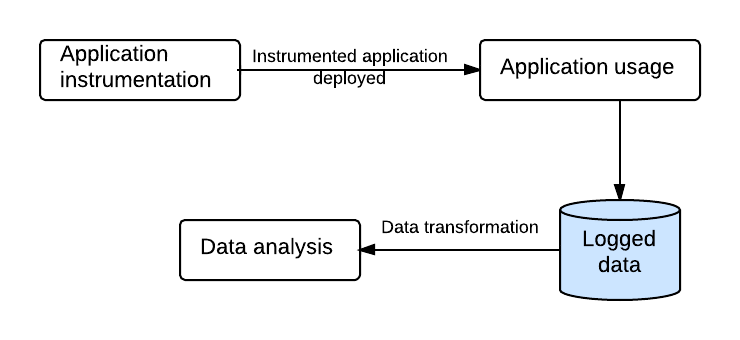
\includegraphics[width=1.0\textwidth]{./images/logging_usability_process.png}
  	}
  	\caption{Process for log-based usability evaluation. \citep{RefWorks:24}}
	\label{fig:logging_usability_process}
\end{figure}

The second stage of log-based usability evaluation process is \emph{the application usage}. It is a stage where the instrumented application is used in an authentic or simulated situation. The log data is collected unobtrusively while the user is performing his or her tasks with the application. \citep{RefWorks:24}

The final stage of the process is \emph{the data analysis}, in which a few different approaches can be used \citep{RefWorks:24, RefWorks:25}:
\begin{itemize}
  \item Synchronization and searching
  \item Event streams transformation
  \item Performance statistics and counts
  \item Sequence detection, comparison and characterization 
  \item Data visualization
\end{itemize}
This part of the process will be described in more detail in the following subsection.

\subsection{Log data analysis}
\label{sec:analysis}
In order to gain beneficial usability information from user interface events, the log data have to be analyzed thoroughly. According to  Hilbert and Redmiles \citep{RefWorks:25}, there are several approaches to sort out important usability information out of log data, and to make it more understandable for humans.
The first one of them is called \textbf{\emph{synchronization and searching}}. 

It is often challenging to interpret user interface events alone and thereby discover valuable higher level events without any contextual information. The purpose of the synchronization and searching is to combine user interface event data with other informative data, such as observations or video recordings, and thereby increase the understanding about the context of use. These two forms of data are complementary and can together provide wider understanding about the usability of a system. Observations or video recordings may provide additional information about the user interface events appeared in the log, or vice versa. However, there are few disadvantages of synchronization and searching techniques. For example, video recording and observation typically require the presence of an observer. Furthermore, using video recording as a part of the evaluation produces a lot of data which can be inefficient to analyze. It might also have a disturbing affect on user's behavior. \citep{RefWorks:25}

The second approach is \textbf{\emph{transformation}}. Transformations combine selection, abstraction and recording to transform events into more beneficial form of information. This information can then be utilized for instance in detecting, comparing or characterizing human behavior patterns. Selection is based on segregating useful information out of mass of user interface related events by filtering out irrelevant data or by selecting the relevant data. Example of a selection could be a situation where the user has been writing a lot of text (and thereby generated a lot of data in the log) and is trying to find save button from different menus. From the usability point of view, text inputs as log events are probably not that relevant, but time consuming browsing between different menus can be a sign of a usability issue. \citep{RefWorks:25}

Abstraction can be used to combine different events into a more understandable event sequences or patterns. For example, a user typing text into different fields and then clicking a button in a web page, could be interpreted as a login activity. However, in this kind of situations the user interface event logs must be supplemented with contextual data, to be assured that the event sequence really is what it seems to be. Recording, on the other hand, means generating new sets of events based on selection and abstraction. Consequently, less effort is required to analyze new sets of raw data because earlier analyzing techniques can be exploited. \citep{RefWorks:25}

The third way of generating tangible usability information out of user interface log data is to use \textbf{\emph{counts and summary statistics}}. Counts and summary statistics are calculations based on usability-related metrics gathered from the log data. For instance, calculating the time spent on a specific task (performance time), can be critical usability information. \citep{RefWorks:24, RefWorks:25}

\textbf{\emph{Detecting, comparing and characterizing sequences}} are approaches which utilize events' sequential information. Sequence detection refers to an action in which ready-defined sequences are tried to be identified from the mass of source sequences. Sequence comparison, on the other hand, is  executed by usability analyst and it is made between two sequences. These two sequences can be generated, for example, according to subject or subject groups. In any case, the purpose of sequence comparison is to compare actual usage against some predefined ideal usage. Sequence characterization applies the source sequences to create a model which summarizes all the features of interest in those source sequences. \citep{RefWorks:24, RefWorks:25}
 
The last approach for log-based data analysis is called \textbf{\emph{visualization}}. In visualization, transformed and analyzed data are  presented in a graphical form. A general way to visualize data is to use charts, but it is possible to use other visualization techniques such as heat maps based on mouse clicks or traveling. \citep{RefWorks:24, RefWorks:25}

\section{Contextual Inquiry}
\label{sec:cinquiry}
Contextual Inquiry is a qualitative data-gathering and data-analysis methodology. It is adapted from psychology, anthropology and sociology. \citep{RefWorks:28} In practice, Contextual Inquiry is an unstructured interview method, but has some qualities which differs it from traditional interviews.\citep{RefWorks:23}  It was originally developed to meet three requirements. Firstly, it was supposed to identify a design process for systems that will be used similarly in different business contexts and in different cultures. Secondly, it was supposed to identify a convenient process to gather user information in limited time, and finally to identify a way to acquire information about users' work in eligible format. In addition to previous requirements, the technique was noticed to be capable of much more. CI cherish participatory design, and because of that quality, the users are able to involve in the design. Users contribute to the design by providing a deep understanding about the nature of the work. This is accomplished through the inquiry, and it is used as a basis for fundamental work concepts. \citep{RefWorks:14} According to Raven and Flanders \citep{RefWorks:28} the Contextual Inquiry was developed in 1986 at Digital Equipment Corporation by human-computer interaction professionals. \citep{RefWorks:28} 

\subsection{Fundamentals of Contextual Inquiry}
Contextual Inquiry can be described as an apprenticeship compressed in time. The basis of the method is premised on the idea about user being the expert instead of the interviewer, but unlike an apprentice, the interviewer neither learns the work by doing it, nor has the same amount of time available for learning. \citep{RefWorks:21} CI differs from the traditional master-apprenticeship model also in many other ways. A few fundamental principles of Contextual Inquiry are said to be essential in order to perceive and overcome the software design problems. \citep{RefWorks:21}. These principles are understanding the context of the work, creating a partnership, interpreting the work, and steering the focus during the interview. \citep{RefWorks:21, RefWorks:28}

Understanding the \textbf{context} of the work is the baseline of Contextual Inquiry. In order to understand the work structure, the interviewer must pursue to perceive the details of the users' work , which can be found by following the users' actions at work. In general, it is important that interviewer avoids gathering abstract or summarized information about the context.\citep{RefWorks:21}

It is essential to create collaborative environment and a \textbf{partnership} between the user and the interviewer, while the real life work structure and activities are tried to be understood thoroughly. Partnership is an equal relationship between the interviewer and the user. In comparison to traditional interview or master-apprentice approach, the partnership doesn't give any power advantage to either of the parties. Instead, it fosters the interviewer's expertise to see the work structure, and the user's expertise to carry out the work. 
\citep{RefWorks:21}

There are many advantages in the partnership approach. For instance, by paying attention to the details and the structure of the work, the interviewer can teach the user to consider them as well. In the best case scenario, the interviewer and the user contemplates about the work structure and design possibilities together. In this case, it is common that the work is suspended while the parties discuss about the work structure, and after a while, returned again. For an interviewer, asking feedback for design ideas is also recommended.\citep{RefWorks:21}

Even though a partnership should be created between the parties, the interviewer should still be able to steer the interview and keep the \textbf{focus} of the conversation on work-related topics, relevant to the design \citep{RefWorks:21}. 

The success of Contextual Inquiry and the system design depends on the gathered facts, but the facts alone are not enough. They are a starting point. \textit{"From the fact, the observable event, the designers make a hypothesis, an initial interpretation about what the fact means or the intent behind the fact."}\citep{RefWorks:21} In other words, \textbf{interpretations} are needed and critical for the success of an inquiry. In the final version of the system, the interpretations have to be correct or the system fails. This is why it is important to share and validate the interpretations with the customer early enough. \citep{RefWorks:21}

There are three types of requirements which should be considered in system development: technical, business strategic and behavioral. The Contextual Inquiry is a part of the Contextual Design (CD) which is a comprehensive design methodology. Contextual Design emerges within HCI, and is used in requirement elicitation focusing on \emph{behavioral requirements}. Therefore, CI can be also used to examine system's behavioral requirements in an authentic environment. \citep{RefWorks:33, RefWorks:36}

As soon as thorough understanding about the work is available, a design for the system model can be created.\citep{RefWorks:14} 

\subsection{Contextual Inquiry interviews}

Practical preparations of CI includes careful planning. The first phase of the planning is to set the focus for the study. Focus can be, for example, a definition of a problem which needs to be solved. It creates the ground rules for the interview and makes it easier for the interviewer to steer the conversation. After the focus has been set, the inquiry itself needs to be designed. The challenge in inquiry design is to find a way to determine underlying issues causing problems in the work. The approach of the design should differ slightly depending on the aim of the inquiry. The possible aims of the CI could be to support upgrading the system, create a totally new system or redesign the process. If CI is used to help the design process of a new system, a challenge is to get the designers and the users to work together, in order to define new ways of working, and to develop a system design to support them. \citep{RefWorks:21} 

The structure of the interview is considerably straightforward. First task of the interviewer is to introduce the CI process to the user and ask permission to record the conversation and the work. The interviewer has to also make it clear that understanding the work is the primary target of the study, and that all the misunderstandings should be corrected. This is called the conventional interview phase. The next interview step is to is to clarify the rules. In the traditional Contextual Inquiry process, it is desirable for the interviewer to interrupt and ask questions, and correspondingly for the user to indicate if the time is inconvenient for interruption. This phase is called the transition. The third part of the CI is the actual interview (the contextual interview proper phase), which consists of observation, asking direct questions, suggesting interpretations, writing notes, and recording the whole chain of events. Finally, the interviewer should wrap up the interview(the wrap-up phase), ensure that everything is understood correctly and summarize the process. This is the last chance for the user to revise the possible misunderstandings. \citep{RefWorks:21}

Contextual Inquiry is usually conducted by one person and the interviewee. If two people are involved, the roles of note-taker and interviewer must be separated. This means that the interviewer is leading the discussion and the note-taker does not participate in it. The approximate length of the interview should be two hours. Additionally, it is important to get an overview of the user's background and demographic information in order to be able to focus on relevant things. It is also important \emph{not to use predefined set of questions}, but to familiarize oneself with the areas of concerns found from the process. Artifacts offering relevant information about the work, such as cheat sheets or notes, should be also collected, photographed or copied. \citep{RefWorks:27} Reviewing the notes is usually required after the interview in order to ensure their comprehensiveness. It is probable that some ideas or impressions might be forgotten during the interview. \citep{RefWorks:28}


\subsection{Data analysis}

The gathered Contextual Inquiry data consist of notes, recordings and possibly artifacts. In order to be able to analyze the data, it has to be in identical format. This is why it might be beneficial to create a summation of the data. It can be accomplished for example by transcribing important notes from the recordings and by describing the artifacts and their use. Once the data are coherent, the analysis can begin. 

The analysis of CI consists of three steps. The first step is to set focus for the analysis. It is often the same as for the inquiry itself, but occasionally insights from the inquiry make the original focus outdated. In this case, the new focus for the analysis needs to be identified again. The next phase of the CI analysis is to choose the data display. There are various methods available, such as affinity and workflow diagrams. After the data display has been chosen, the final step is to organize the data in it. \citep{RefWorks:28}

The affinity diagram organizes single notes in to higher categories or hierarchies. No predefined categories exist in affinity diagram for individual notes. Instead, single notes are used to define a category and then the corresponding notes are being attached to the same category. In other words, the notes create categories and categories then raise common structures and themes. After the categories or groups are formed, and there are no floating notes left, the groups have to be named descriptively. Additionally, groups of the groups are being collected, and thereby hierarchies are created. The named groups, hierarchies and their headings represent new information in an affinity. \citep{RefWorks:21, RefWorks:28}

The workflow diagram can be used if the work process needs to be tracked and understood thoroughly. At first, the notes from each interview need to be reviewed, after which the flow charts can be conducted. The flow charts should reflect the work process of each individual of every interview. Afterwards, all the flowcharts need to be displayed and compared. Finally, a composite workflow diagram (containing the stages perceived in most of the inquiries) can be created. \citep{RefWorks:28}

\subsection{Remote Contextual Inquiry}
The possibility to remotely evaluate the usability of a system was already discussed earlier in this study (see section \ref{sec:rue} \nameref{sec:rue}). The Contextual Inquiry can be also implemented remotely with a few modifications on the traditional on-site approach. The remote version of CI is called Remote Contextual Inquiry (RCI). It aims to create a bridge between the users and the developers. It is particularly effective when a project requires feedback from users in distributed locations. RCI is a considerable option, when the preparation time is limited and the cost of the evaluations is an issue. It can be set up and conducted in less time than the traditional Contextual Inquiry. \citep{RefWorks:32}

In practice, RCI captures the screen of the user's work with a suitable software, and the usability professional is in contact with the user, for example via teleconference application and shared screen. Otherwise, the activity is basically the same as in traditional CI: User works with the tasks and usability professional observes, records the usage, and gathers information about the real-life usage of the system. The analyst also probes and discusses with the user. \citep{RefWorks:32}

The results of the RCI are versatile. Information about the users' goals and the actions required to achieve those goals can be captured together with the elapsed time and the number of keystrokes. Moreover, RCI provides feedback on layout, content and behavior of the system. \citep{RefWorks:32}
 
\section{Cognitive Walkthrough}
\label{sec:cognitivewalkthrough}

Cognitive Walkthrough (CW) was developed in the early nineties and it was originally intended to help reviewing 'walk-up-and-use' interfaces, such as Automatic Teller Machine (ATM). CW is a formal usability inspection method for professionals involved in the development process. The key concept behind CW is to use theory as a guide for design review. It is easy to understand and apply and therefore feasible to use in a regular development process. \citep{RefWorks:19, RefWorks:18} Cognitive Walkthrough is an additional tool for usability engineering and it can be used for quick evaluation of mock-ups or design sketches. \citep{RefWorks:34}

\subsection{Fundamentals of Cognitive Walkthrough}

In theory, human-computer interaction process can be described in four steps. Firstly, the user sets the goal for the activity which is to be accomplished with the system. Secondly, the user examines the user interface for available actions. Thirdly, the user selects the action most likely to make the progress. Finally, the user carries out the action and assess the feedback from the system. In real-life tasks, these steps would probably iterate to achieve subgoals and to complete tasks. Cognitive Walkthrough examines the correct actions to accomplish a task and the four steps to carry out those actions. \citep{RefWorks:34}

Cognitive Walkthrough consist of two phases: preparatory and analysis phases. The preparatory phase contains prerequisites for the walkthrough. The first of them is a brief description of the user and the knowledge he or she possesses. The second prerequisite is a specific description of one or more tasks to be carried out with the system and the last one is a list of correct actions required to complete the tasks with the UI. The actual analysis will be accomplished in the analysis phase, where every action of every task will be executed and analyzed. In general, the Cognitive Walkthrough method can benefit all phases of system's design and development process.\citep{RefWorks:26, RefWorks:34}

\subsection{Preparations}
Cognitive Walkthrough can be accomplished by utilizing the user interface's detailed design specification which has been composed after the system requirement analysis and functionality definition processes. The walkthrough can be also performed on a paper simulation, minimal prototype or fully functional prototype of the UI. Formally, Cognitive Walkthrough evaluates the ease of learning by exploring it. \citep{RefWorks:26}

The analysis can be completed individually or in a group. In a group the process starts by designers presenting the design to a group of peers, and it's usually completed after a certain milestone in interface design. The designers can benefit from the feedback and improve the implementation for the next revision. Participants may represent different organizational units and they have to adopt different roles in the evaluation team, such as recorder, facilitator and various kinds of expert roles. \citep{RefWorks:26}

The first step of the walkthrough preparations is to describe the users of the system, and to choose the tasks for the analysis. If the background and technical experience of the users are described in the beginning, more details can be possibly revealed in the walkthrough itself. \citep{RefWorks:26}

The selection of tasks (for analysis) is critical and should be based on facts, such as requirement analysis, demand analysis or concept testing. The amount of tasks should be moderate, and it is important that the set of chosen tasks includes some core functionality and some combinations between those core functionalities. Furthermore, to make the tasks as concrete as possible, context descriptions and task stages should be included in the preparation documentation. \citep{RefWorks:26}

After the tasks have been chosen, the action sequences for the tasks need to be described. Basically it means that the sequence of actions, which are required to accomplish the task with the UI, are being described. These actions can be as simple as "press the start button" or "write your name in the text field". However, depending on the level of user expertise and user descriptions, actions might also consist of several simple actions which can be executed as one block. These kind of actions could be, for example, filling in the register form or going to a specific website. The interface definition should include the prompts preceding all the actions in the task, and the interface's reactions to those actions. If the development is already finished, all the information about the interface is available, but if the development process is just in the beginning, documentations are needed. \citep{RefWorks:26}

\subsection{Analysis}

The analysis phase examines the actions of the tasks and generates a plausible story or a review about the reasons why the users (which have been defined earlier) would have chosen those actions. These stories are based on presumptions about users' expertise and objectives. \citep{RefWorks:26}

Occasionally, users trust their problem-solving skills, hence it is important to understand the problem-solving process in the analysis phase. In order to mimic this process in the analysis phase, four steps should be taken. First, a rough description of the task to be accomplished should be considered. Then, the user interface should be explored and actions should be taken according to assumptions the users might have. The third step is to observe if the user interface is returning the expected results for each action. The last part of problem-solving process is to assume and define users' next actions.\citep{RefWorks:26} In general, the walkthrough, or the analysis evaluates if the user is able to select the correct actions with the user interface.

Four criteria can be used in order to assess the ease of performing the correct actions and thereby completing the task. According to the criteria, the goal, the accessibility of the correct user interface object, the match between the label of the object and the object itself, and the feedback provided, should be considered while evaluating the system. \citep{RefWorks:34}

The analyst should ask the following questions while going trough the task sequence or different stages on it. The questions should be used as a guidelines or criteria for creating a credible story about the interaction between the user and the system. \citep{RefWorks:26}
\begin{itemize}
\item Will the user try to achieve the right effect?
\item Will the user notice that the correct action is available?
\item Will the user associate the correct action with the effect they are trying to achieve?
\item If the correct action is performed, will the user see that progress is being made toward solution of their task?
\end{itemize}

The first question should be asked to make sure that the users would understand the actions required to proceed. The second question, on the other hand, aims to ensure that the user can notice that all the relevant actions are available.
The third question should be asked to perceive poor naming of the actions and the last one to ensure that the necessary feedback is provided for the user. 

The story created in the analysis should include credible success stories and failure stories. The success stories are being created when the system works and the users could credibly proceed from one task stage to another. If the credible story cannot be created, and the story fails under the criteria, failure story should be included in the analysis and it should provide a description why the users would face the problem. Utilizing the stories, system's advantages and disadvantages can be described. \citep{RefWorks:26} 		

\section{Interaction Sequence Illustration}
\label{sec:isi}
Interaction Sequence Illustration is a modified usability inspection method. It differs from the traditional inspection methods, such as Cognitive Walkthrough and heuristic evaluation, in a significant manner. Unlike other inspection methods, ISI does not function in isolation from system's actual context and users. It conducts the model of interaction from the real-life environment. If multiple systems are required to perform the user's task, ISI can also focus on many systems instead of just one, and thereby detects the whole use sequence. In general, ISI combines user-based testing and usability inspection approaches. The method was originally developed for evaluating the usability of Information Technology (IT) tasks carried out in the health care industry, but there are no defined reasons why it could not be utilized in different environments as well.  \citep{RefWorks:17} 

\subsection{Description of the Interaction Sequence Illustration}
Interaction Sequence Illustration focuses on low level analysis of human-computer interaction and exploits the data acquired during the Contextual Inquiry process. However, the inquiry data have to be complemented with the documentation about interaction activities, photos and screenshots. There are three objectives for ISI method to handle. The first is to demonstrate how the user perceives the system. The second is to identify and document activities, and to discover problems. The first two objectives form the basis for the third and more extensive objective, which is to support the user-centered design and development. \citep{RefWorks:17}  The strength of ISI lies in the analysis of data and it can be used to compare the interaction sequences of two or more UI implementations. On the other hand, it can provide prominent information on only one UI's interaction sequence. 

ISI generates two analysis from the collected data. The first one is an analysis of interaction stages, which divides the whole interaction sequence in to main phases or stages. The analysis is performed based on the inquiries. The second analysis is so called step-by-step illustration. It defines the stages and interaction steps by numbers, photos, descriptions and screenshots. \citep{RefWorks:17} It is basically a well defined and ordered workflow description. 

\subsection{Application of the Interaction Sequence Illustration}
The utilization of Interaction Sequence Illustration can be simplified in seven steps (see figure \ref{fig:isi_chart}). Firstly, the data need to be collect alongside a Contextual Inquiry interview, including inquiry data, possible photos, screenshots and notes.
After the data has been collected, the screenshots need to be arranged in the chronological order and all the superfluous data need to be removed. The third phase is to count the interaction steps based on the screenshots and activity analysis, and to organize interaction steps into stages.
Next, the screenshots need to be modified and important details highlighted. Finally, the sequence numbers and  detailed description texts should be attached to the screenshots in order to give a profound understanding about the actions. The outcome of the method is an extensive illustration of the interaction sequence, information about the usability of the system, and about it's effectiveness of use. \citep{RefWorks:17}
	
\begin{figure}[H]
  	\centerline{
  	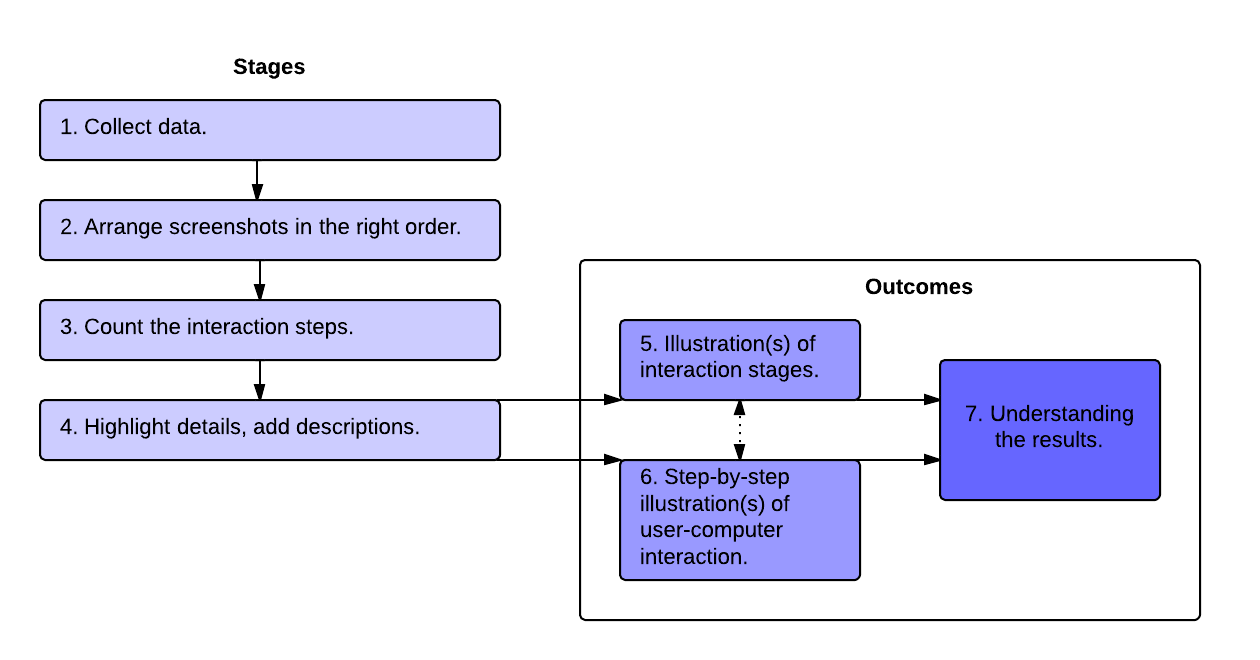
\includegraphics[width=1.3\textwidth]{./images/isi_chart.png}
  	}
  	\caption{Interaction Sequence Illustration stages and outcomes.}
	\label{fig:isi_chart}
\end{figure}

\section{System Usability Scale}
\label{sec:sus}
In his paper, Brooke \citep{RefWorks:10} argued that usability is not any real existing quality, but a good usability artifact is \emph{appropriate to its purpose}. In other words, "the usability of any tool or system has to be viewed in terms of the context in which it is used, and its appropriateness to that context"\citep{RefWorks:10}. Still, in many cases, context related usability evaluation is not necessarily desirable. The reason for it, is that a large scale context analysis is usually neither cost-efficient nor practical.\citep{RefWorks:10} In the 1986, System Usability Scale was introduced to respond these challenges by offering "quick and dirty"\citep{RefWorks:10} way to get subjective ratings about the usability of a system. \citep{RefWorks:12, RefWorks:35} System Usability Scale can be also used as a supplement for other usability evaluation methods.




\subsection{Numbers behind the System Usability Scale}

In their study, Bangor et al. gathered results from 206 SUS studies consisting of 2324 surveys. In the general overview, the study reported the nature of the SUS by providing understanding about the value range for good and poor usability. The study indicates that the mean value of all the surveys were 70.44, the median value was 75, and one fourth of the scores were 55 or less (pointing out the weakest quarter of the results). According to the study, one of the best qualities of SUS is that it is not dependent on any specific technology or user interface type. Thereby, it can be used to evaluate the usability of wide range of different kinds of interfaces from traditional desktop user interfaces to mobile web UIs. However, the study found significant differences between various user interface types. \citep{RefWorks:12}	

The reliability analysis was also implemented in the study. It was executed by calculating Cronbach's alpha from the ratings. The calculations indicated that the result of the analysis was 0.911, which makes the SUS analysis' internal consistency, and thus the reliability, excellent. However, like any other usability method, SUS should not be used in isolation, but as a part of the overall evaluation. \citep{RefWorks:12}

The study illustrates six major ways to benefit from the utilization of SUS. \citep{RefWorks:12}
\begin{enumerate}
\item It provides a single measure of customer satisfaction and usability.
\item It can be used to compare different tasks of the same interface. 
\item SUS can be used to compare different versions of the same system.
\item Competing implementations can be compared by means of SUS.
\item Competing implementations with the same functionality (e.g. competitor's products) can be compared by means of SUS.
\item SUS can be used to compare different interface technologies.
\end{enumerate}

The remarkable question of SUS is: what is a reasonable score? According to the research study, there is no unambiguous answer available. The criteria for good usability differ greatly between industries and the products' life cycle states. However, an organization consistently collecting the SUS data certainly has an understanding what the scores mean for them. Still, the collected data in the research study indicates that passable products have the SUS score of 70, better products have the score from high 70s to upper 80s and superior products the score above 90. Products with the SUS score under 70 should be improved and the ones with score less than 50 should be considered as unacceptable. \citep{RefWorks:12}

\subsection{Practical implementation}
System Usability Scale is a ten-item \emph{Likert scale} (see \nameref{app:susform}), meaning that every item consist of scale of five, ranging from "Strongly disagree" to "Strongly agree". The questionnaire should be filled right after the possibility to use the system to be evaluated. The focus should be on immediate responses and too much time shouldn't be given to the respondents. SUS is relatively fast to implement by administrators and to use by the study participants. \citep{RefWorks:10} 

The outcome of SUS is a single value which express the overall system usability. The value of the method consist of all the items and none of them are meaningful as such. System Usability Scale can be calculated by summing the score contribution (range from 0 to 4) 		from each item. Before summing the scale positions, the items 1,3,5,7 and 9 need to be subtracted by one and the items 2,4,6,8 and 10 need to be subtracted from 5. The last step is to multiply the sum of the scores by 2.5 to get the overall SUS value, which range from minimum of 0 to maximum of 100. \citep{RefWorks:10} The resulting single score is an easy-to-understand measure, and can therefore be discussed about with the wide range of stakeholders. \citep{RefWorks:12} 
    
\chapter{Outline and implementation of the study}
\chaptermark{Outline and implementation}
\label{chapter:implementation}

According to the ISO standard 9241-210, human-centered design consists of a few activities and an iterative process (see Figure \ref{fig:hci_process}). \citep{RefWorks:40} The empirical part of the Master's thesis adapts human-centered design principles. The steps of the process experiment are highly linked to its activities. The rationale for adapting human-centered design is to study how standardized human-centered activities fit in the company's software development process. The human-centered design and the selected methods are represented as a part of software development process in figure \ref{fig:lm_process}. It also defines the fundamental idea behind the Master's thesis: Trying to improve in-house software development process by introducing human-centered activities and methods.

This chapter contains description about the principles of human-centered design. The applied steps of the research are described in section \ref{sec:dprocess}. Additionally, the chapter describes the implementation phases of the study. 


\begin{figure}[H]
  	\centerline{
    	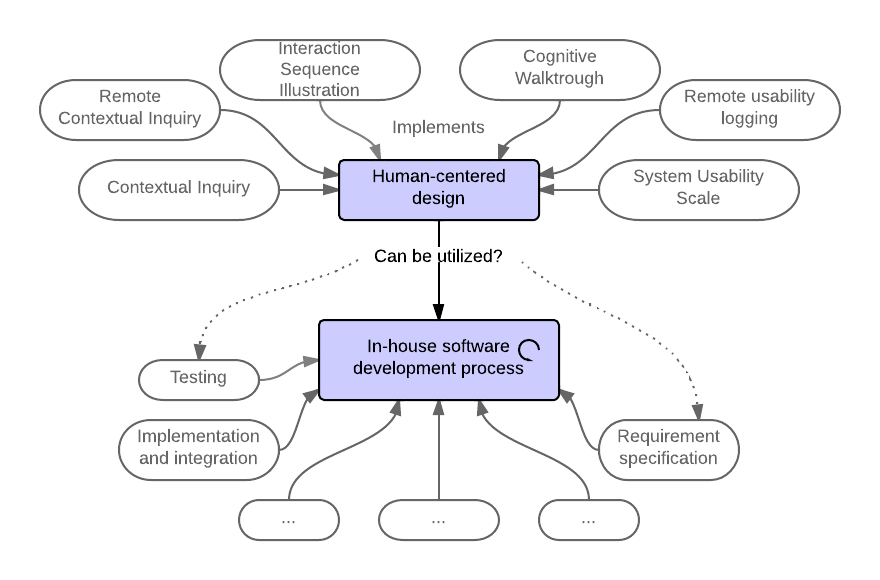
\includegraphics[width=1.2\textwidth]{./images/lm_process.png}
    	}
  	\caption{Human-centered design as a part of in-house software development process.\citep{RefWorks:40}}
	\label{fig:lm_process}
\end{figure}


\section{Principles of human-centered design}
\label{sec:principles}
Human-centered design does not require any particular design process and functions as a supplement to existing design methodologies. However, a few principles should be followed in order to make the process human-centered. \citep{RefWorks:40}

Firstly, understanding the users, tasks and environments should create the basis for the design. In other words, all the user groups and stakeholders affected directly or indirectly by the developed system, should be considered.
Secondly, the users should be actively involved in the design and development processes in order to provide essential information about the context of use and the practices of work. The people participating in the processes should possess comprehensive understanding about the work and should be able to represent wide range of users. Thirdly, the design should be driven and refined by user-centered evaluations. This means that the feedback from user evaluations should be used as a basis for improving the design. This approach efficiently minimizes the risk of system not meeting the requirements, including hidden and implicit requirements. \citep{RefWorks:40}

Fourthly, the process should be iterative. It is impossible to define all the user requirements in the beginning of the system development. This is why iterative revision and refinement of the descriptions, specifications and prototypes is required. Additionally, iterative development eliminates uncertainty during the development. Fifthly, the design should encompass the whole user experience (consisting of set of factors such as presentation, functionality, performance and interaction). Designing the user experience should not ignore supporting matters like training, documentation and long-term use or user group's qualities, such as previous experience, attitudes, skills and habits. Moreover, deciding the extend of automated functions in the system should be a process considering users' strengths, limitations, preferences and expectations. Additionally, things such as reliability, speed, accuracy, financial cost and safety should be reflected upon before making such decisions (together with the user representatives). If the design involves the whole user experience, the outcome should be meaningful for the users as a whole. \citep{RefWorks:40}

Finally, the design team should consist of multidisciplinary individuals. A good skill set for a project team may consist of usability engineers, users, application domain experts, marketing experts, user interface designers, technical writers, business analysts, software engineers and human resources experts. Project benefits from the collaboration of multidisciplinary individuals, and moreover, the members of the teams can become more aware of the constrains and realities of other disciplines. \citep{RefWorks:40}

\section{Applied human-centered design process plan}
\label{sec:dprocess}

The subscriber company has a local customer service department in every country it operates and those departments are in charge of customer creation process to the ERP system. The employees of the customer services also modify the customers' information in order to keep them up to date. Updates require daily actions to the system, such as editing delivery addresses, renewal settings or invoicing frequencies. The accuracy of the customer information in the system is obviously highly important for the business. Consequently, the study examines the customer information processing (creation and modification) throughly and uses it as an example to improve the existing software development process.

\begin{figure}[H]
  	\centering
    	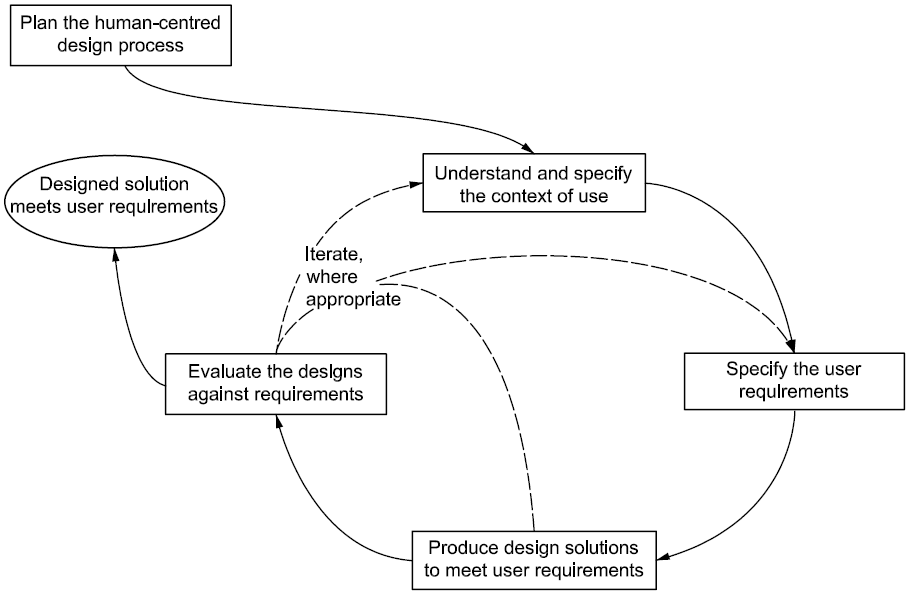
\includegraphics[width=1.0\textwidth]{./images/hci_process.png}
  	\caption{Human-centered design activities.\citep{RefWorks:40}}
	\label{fig:hci_process}
\end{figure}



The following section forms the first activity of the human-centered design, called \emph{planning the design process}. The section applies the activities of the human-centered design and creates a proposal of methods and procedures to be introduced in the company's software development process. The section also provides the reasoning for the created proposals.

The examined ERP process is accomplished by the personnel expertized in the area of customer service, and the primary tool for the process is company's tailored ERP system. Moreover, the distinctive nature of the business sets additional challenges for the usability evaluations. This is why it is presumable that the process can not be understood thoroughly without understanding the work in practice. Because of the reasons mentioned earlier, Contextual Inquiry and Remote Contextual Inquiry are selected as main methods for \emph{understanding and specifying the context of use}.

The researcher must have a profound understanding about the context of use, in order to \emph{specify the user requirements}. A qualified system can be implemented only if the user requirements are precisely defined. Many of the applied methods aim to assist in this crucial state of development. Technically, the process of requirement specification can be initiated while running the Contextual Inquiry or Remote Contextual Inquiry. Although, it is essential to remember that the focus in CI and RCI should be (at the first stages of the process) mostly on understanding the context of use. This Master's thesis applies user evaluation, remote usability evaluation, expert evaluation, and qualitative metrics to identify all the user requirements affecting on the user experience and the system functionality.

Interaction Sequence Illustration method is used to identify and represent the interaction steps required to accomplish the customer creation process with the system. The method was chosen because one of the main objectives of this thesis is to find out what usability methods can be practically joined with the development process, as well as to improve end product's quality and make it more efficient. ISI can be used not only to identify all the interaction steps, but to detect the unnecessary steps as well. If the unnecessary phases can be excluded from the process, it might have significant affects on the efficiency of use and reveal tacit user requirements. 

The user experience might have an influence on use efficiency. This is why the UX should be also considered in the development of distinctive ERP system for experts. Additionally, System Usability Scale is being used to understand the level of user satisfaction which is highly connected, among many other factors, with the user experience.

Traditional and continuous usability evaluation would be difficult and expensive for the subscriber company, because of the distributed operational environment. Hence, the possibility of accommodating remote usability evaluation as a part of company's software development process is examined as a part of this Master's thesis. The remote usability methods applied in the study are the remote usability related user interface data logging and the Remote Contextual Inquiry. The desirable results from the data logging and RCI are supposed to be applicable, localization dependent usability data, which may contribute to the development of the global ERP system, and to reveal cultural dependent user requirements. 

Expert evaluation is accomplished by applying Cognitive Walkthrough. The objective of CW in the study is to identify user requirements which are not distinctive, and cannot be noticed with the other usability methods. The Cognitive Walkthrough is used to ensure thatthat none of the crucial requirements will be omitted.

After the specification of the user requirements, \emph{a design solution can be produced according to these requirements}. Analyzed data are applied to create a new user-centered prototype solution. Later, the solution and \emph{the design is evaluated against the requirements}. Mock-ups are used to evaluate the design solutions before the implementation of the high-fidelity prototype.

Figure \ref{fig:hcd_process} illustrates the utilized methods and the performed actions in the applied design process and reflects the way they differ from the general human-centered design process. Contextual Inquiry, Interaction Sequence Illustration, System Usability Scale and Remote Contextual Inquiry are applied to understand the context of use and the current solution's level of sophistication. The same methods in addition to Cognitive Walkthrough, are applied to specify the user requirements. After the examination of the current system and prototype creation, the design solutions and the prototype UI are evaluated by applying the Cognitive Walkthrough, ISI, RCI, remote usability data logging, and System Usability Scale. The final analysis is carried out using the data from the second evaluation.  

The applied human-centered design activities described in this section could be attached to iterative software development without an effort. In practice, the following iterations would create only few changes in the applied process and in the set of utilized methods. Contextual Inquiry and Remote Contextual Inquiry could be used to identify the issues which need to be improved in the following iterations. System Usability Scale could be used to gather data about the improvements in order to understand their consequences. The SUS could probably be even more useful in the following iterations, since there would be earlier scores available for comparison. Interaction Sequence Illustration could give beneficial information during the first iteration about the quantitative changes in interaction stages and steps and about the complexity of the interaction. However, it is likely that in a long run it would get ineffective if the iterative updates would be small and no changes would be made in the interaction sequence itself. Although, if the software development iteratively increments the number of processes attached to the system, then ISI can be applied in every iteration to assess the difference between the current and new process implementation. Remote usability logging could be used during the iterations to gather quantitative information and therefore assessments about the success rate of the iteration. Cognitive Walkthrough could be used as an anticipatory test for the iteration before the update is published. 

It is noticeable, the focus of the methods can vary also inside an iteration. For example the second stage of the applied design process utilizes Contextual Inquiry to understand the context of use, whereas the last stage applies CI to evaluate the design against the requirements. 

Altogether, the only changes between the initial iteration of the applied human-centered design and the following iterations would be that the Interaction Sequence Illustration would possibly get decommissioned, and the other methods would be used from slightly different perspectives. 

\begin{figure}[H]
  	\centerline{
    	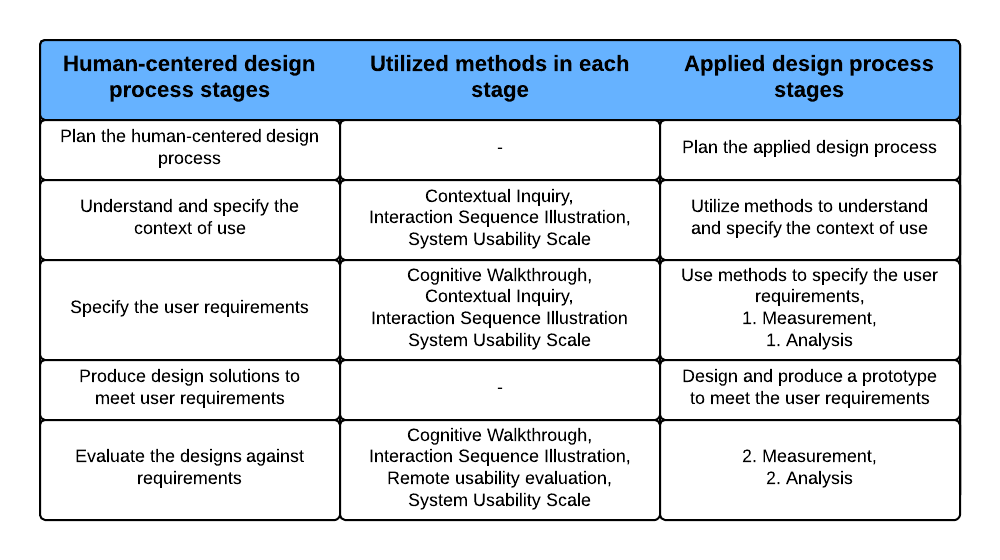
\includegraphics[width=1.3\textwidth]{./images/applied_hcd_process.png}
    	}
  	\caption{Relations between human-centered design process stages, methods utilized in the thesis and the implementation stages of the thesis.}
	\label{fig:hcd_process}
\end{figure}



\section{Practical implementation of the applied design process}
 \label{sec:implementation}

    
The practical implementation of the research study took place between August 2013 and January 2014. Altogether, seven users from two different countries contributed in the study, by participating in the usability evaluation sessions. The following usabiliity evaluation methods were applied: remote data logging, Contextual Inquiry, Remote Contextual Inquiry and Interaction Sequence Illustration. In addition, the users filled out the System Usability Scale form. The only usability inspection method that was utilized by one analyst was the Cognitive Walkthrough.

The chosen process for the research study was considered carefully. Due to the limitations of the time schedule, the process had to be restricted. What is more, it had to be noticeable part of the system, with the option to track qualities such as average processing time and number of interaction steps. Finding an applicable system segment proved to be a challenging task, partly because of the tailored nature of the ERP system. Eventually, the customer management process was chosen because it was seen as an appropriate part of the system to be studied. What is more, the customer management process has some anticipated usability issues (in the old system) and it is considered as an important part of the future ERP system.

In practice, one applied human-centered design iteration was divided into three main phases, containing all the stages of the applied human-centered design process: two evaluation rounds and one implementation round. The aim of the first evaluation round was to gain understanding about the current system, including its deficiencies and assets. The focus to understand the process and the way users are utilizing the system in their everyday work. After gathering the basic understanding of the process, the system's capabilities and issues, a highly limited prototype of the new system was created utilizing up-to-date technologies. The objective of the second evaluation was to assess the prototype and redefine the new system requirements (gathered during the first evaluation round). 

\subsection{Current system evaluation}
\label{sec:firstiteration}

The first evaluation round encompassed the Contextual Inquiry, Remote Contextual Inquiry, System Usability Scale, Interaction Sequence Illustration and Cognitive Walkthrough. Contextual Inquiry was utilized first with the ISI method in Finland, aim was to gain understanding about the context of use. Overall four users participated in the inquiries and they presented all the experience levels available in the work community. The employment period in the company varied from half a year to 21 years with an average of nine years. The age and technical background of the users varied considerably as well. Moreover, each of the users worked in the customer service and was managing the customer details daily or weekly, so each of them had relatively good understanding about the process. The users were situated on their workstations and if real-life cases (customer creation) were available, they were used as a basis for discussion. However, because of the lack of variety of authentic cases, the users were provided access to the test environment of the present ERP system. The aim was to enable the users to manage customer information without a risk of interfering with the real customer data. The inquiries lasted approximately two hours each, following  the traditional Contextual Inquiry form. At the end of each inquiry, the users were asked to implement a customership with the predefined customer details. The details were tried to be specified according to real-life cases and to be as all-inclusive as possible. In effect, it was possible to gain understanding about the whole customer creation process and to collect data for Interaction Sequence Illustration. The inquiries were documented with the voice recorder and the Interaction Sequence Illustration tasks were recorded with a high-definition video camera. Additionally, notes were written during the interviews.

The second stage of the first evaluation round was to apply Remote Contextual Inquiry in order to interview three Swedish users, and gather cultural independent customer management data. The users were selected according to the same motives as in Finland: to get the viewpoints of diverse user types. The Swedish users work experience varied from half a year to two years in the company, with an average of 1.33 years. The Swedish users were also dealing with the customer details daily or weekly. The inquiries didn't differ from the inquiries implemented in Finland in any other way except that the inquiries in Sweden were carried out remotely and that the technical equipment were different. The interviews were conducted by utilizing web conferencing software, which allowed desktop sharing, voice conferencing and recording of the whole interview. The users were using the present system as they usually would except from the fact that their screens were captured. At the end of each inquiry, the users were asked tocarry out the same tasks as the Finnish users, in order to gather data for the ISI method. Notes were made during the  interview sessions.

After the inquiries, Finnish and English versions of the SUS form were sent to the users as a web form, and Cognitive Walkthrough was implemented. The forms were sent to the users after the inquiries, in order to give them preceding information on what the forms' results will be used for. Cognitive Walkthrough was implemented after the inquiries as well, in order to ensure the capture of the critical information before the prototype implementation. The inspection was executed in the system's test environment, according to the instructions of the method. The results were gathered by reviewing the guideline questions of the method and by documenting all the success and failure stories. 

The overall analysis of the first evaluation round was made after all the evaluation data had been gathered  (see chapter \ref{chapter:analysis}). 

\subsection{High-fidelity prototype and remote usability logging library implementation}

The development of the prototype started by creating a new design for the interface. It was accomplished by sketching a few mock-ups. The mock-ups were built by using the storyboarding tool provided by Microsoft's Visual Studio Ultimate 2012 Integrated Development Environment (IDE) and evaluated with three customer service specialists in Finland. After the evaluation and refinement of the design in multiple meetings, the prototype creation began.

The prototype was built based on the outcomes of the first evaluation round, and the results mock-up evaluation meetings. It was implemented with the Microsoft's .NET 4.5 software framework. Because of the organizational and time schedule requirements, the prototype was implemented as a desktop application without any real back-end solution. The user interface was created with Windows Presentation Foundation (WPF) and C\#, utilizing the Model View ViewModel (MVVM) presentation pattern in order to achieve Separation of Concerns (SoC). \citep{RefWorks:37} Furthermore, third party components were applied in the implementation in order to create the prototype more efficiently. The prototype was filled with dummy data, which were gathered from the current ERP system. All of the functionalities were not fully implemented due to the time schedule limitations and the extensive scale of the functionalities available in the real system. However, lot of dummy functionalities were created in order to make the prototype more authentic.

A few solutions were reviewed in order to be able to utilize remote usability logging methodology. The third party solutions were not seen as cost efficient, which is why a code library for remote usability logging was implemented as a part of the study. The library consisted of a singleton pattern and static methods which were build on a Windows Communication Foundation (WCF) service and Microsoft's SQL server database. The library provided methods for logging sessions and events during the user interface interactions, and saved the data to the database. The prototype referenced the library and the user interface code was  decorated with the remote logging code snippets.

The logging functionality gathered session data such as name, version and user of the application, as well as the start and end times of the session. In addition, it captured the state of arbitrary objects in the beginning and the end of each session as serialized the object as Extensible Markup Language (XML) data. The tracked event data consisted of the name and version of the application together with the tracked feature description, link to the session and start and end times of the event. Similar to session tracking, the library also tracked serialized arbitrary object data in the beginning and end of an event.

	  
\subsection{Prototype evaluation}

The second evaluation round differed slightly from the first one. The prototype was presented to the users in the beginning of the each evaluation session. In order to make the presentation pragmatic, some dummy data were inserted to the prototype. However, the users were also able to enter the data to the prototype themselves. The evaluation round started with a short evaluation meeting with the Finnish users, to ensure that the mock-ups and the prototype design corresponded to each other in a general level. Additionally, the Cognitive Walktrough was implemented to ensure that all the critical issues in prototype could be eliminated as carefully as possible. The purpose of the evaluation was also to find out if the analyst, who was creating the prototype, was able to discover any flaws after the implementation, by applying the Cognitive Walkthrough. The evaluation was implemented correspondingly to the evaluation of the current system version. 

The prototype was evaluated with the Swedish users using Remote Contextual Inquiry. The participants of the inquiries were the same persons as in the first evaluation round and the pattern of the inquiries were highly similar. The only difference was that the prototype was introduced thoroughly to the users in the beginning of the interviews. The screen was shared and the interviewer proceed on the UI sections one by one. Later, the user was asked to share the screen and run the prototype application. At the end of each inquiry, the user was asked to create a customership with the predefined details and by using the prototype. The aim was to gather data for Interaction Sequence Illustration evaluation purposes and to find some critical problems with the interaction. The predefined customer details were not identical to the ones applied during the first evaluation round because of the different design approaches of the same functionality. However, the aim was define the details and the task as all-inclusive as possible. 

Remote usability logging was applied during the inquiries to count the time consumption of the sessions and events, as well as to examine the functionality of the library and its suitability for usability evaluation purposes. The session was started in the code when a user created a new customer and ended when the user clicked Save-button. Events were recorded, for example, when the user created a new contact for the customer. After the inquiries, English version of the SUS form was sent to the users to rate the prototype.

The overall analysis of the second evaluation round was made after all the evaluation data had been gathered  (see chapter \ref{chapter:analysis}, \nameref{chapter:analysis}). 
    	
\chapter{Analysis and results}
\label{chapter:analysis}

This chapter summarizes the Master's thesis and presents its results. The first section of the chapter describes the adopted analytical methods, whereas the second section summarizes the results from the usability evaluations, and presents the user interface prototype solution created. The last section of the chapter discusses about the implementation guidelines of the applied human-centered design process. 

\section{Analysis description}
\label{sec:analysismethods}
The analysis was implemented in two phases, analyzing the present ERP system and the new prototype. The first phase of it was conducted after the first evaluation round and before prototype design. The Contextual Inquiry and the Remote Contextual Inquiry focused on analyzing the context of use and the users' procedures concerning the current ERP system. Affinity diagrams were chosen for data display in the analysis and the study material gathered (videos, recordings, photos and notes) was examined and organized into wider categories, which implicated the results of the first inquiries. 

The Cognitive Walkthrough analysis was completed (after gaining understanding about the context and usage) by generating a plausible story of how the users could behave while creating or managing the customership. The UI was explored and actions were taken according to the assumed user behavior. During the exploration, the system responses were monitored and success and failure stories were gathered according to the guidelines of the methodology. System Usability Scale analysis was accomplished by counting all the anonymous results according to the formula. All data from the first evaluation round, gathered from Finnish and Swedish users, were analyzed separately, in order to detect the possible differences between the working habits.

The Interaction Sequence Illustration analysis was implemented by reviewing the recorded video material, taking screen shots  and making calculations from the material that was already entered into the system. Counting and analyzing the interaction steps proved to be more complicated than expected. The reason for the complication was the varying amount of customer details, received from the customers themselves, and the changing requirements between the customers. As a solution, 50 random customership details were examined and the average amount of interactions was calculated together with the highest possible interaction amount enabled by the system. Additionally, by utilizing the video recordings and knowledge gained from the inquiries, it was possible to capture the main interaction stages required for the customership creation process. Due to the wide extents of customer details and customer requirements, the original plan to measure the time required for the interactions (customership creation) and to compare with the results from the current system and the prototype became impossible. 

The second phase of the analysis applied methods similar to the first one, with a few exceptions.  On the second round, the focus of the inquiry analysis was on redefining the requirements and design solutions, and the Interaction Sequence Illustration focused on capturing the stages of the customer creation process. The problems faced in the earlier phases of the analysis made it also impossible to calculate the specific amount of interaction steps of the prototype and therefore fully utilize all the advantages of the method. Naturally, there were no previous data about the prototype, so it was also impossible to calculate any data averages. For the same reasons, the analysis of the remote usability logging focused mostly on its possibilities in measuring the system usability. 


\section{Study results}
\label{sec:results}
This section reviews the results of the thesis. Firstly, the results gathered by evaluating and analyzing the data of the current ERP system will be presented. Secondly, the overview of the prototype's user interface solution will be given, and the differences between the present system and the prototype UI will be discussed, in a general manner. Finally, the section concludes with an outline of the prototype usability evaluation results. 
    

\subsection{Results of the current system evaluation}

The Contextual Inquiry was selected as a first method to evaluate the present ERP system. Regardless of the lack of the real-life customership implementation cases, a significant amount of ideas, critical problems and usability issues were gathered during the inquiries. 
In Finland, the four implemented inquiries resulted overall 57 different notices. In affinity diagram analysis, the notices were sorted into groups based on their natural qualities. From the large mass of data six different categories emerged. 

First category was named as critical problems. Overall four different notices were classified as critical problems. Critical in this context stands for harmful issues which affects on business in a debilitating manner and can cause financial loss. In general, all the problems were caused by system not being responsive enough and leaving some critical notes out of interaction, or by system's lack of automation. The second category was named as naming issues. The number of naming issues found from the customer management of the system, was six and all of which were found from the user interface buttons, selections and labels. The naming in these cases were generally misleading and caused some extra memory load for the users. In few occasions some users were not able to recognize what the functionality stood for, because of the poor naming conventions. 

The third category holds the greatest amount of problems gathered from the inquiries in Finland and was named as customer hierarchy problems. The hierarchical problems originated mainly from the different customer levels and a total of twenty different issues were found. From the usability point of view the biggest problem with the hierarchy was probably it's lack of adjustment according to the customer levels. This means that the same preferences were available in every customer level of the system, even though they weren't needed on that specific level. What is more, the hierarchy itself was possible to break, which in worst case could lead into financial losses. Additionally, hierarchical inheritance of the preferences in the system were not defined accurately enough, and their correctness were based on users memory and experience. The next category found was named as user interface issue and total of fourteen issues were categorized as part of it. The problems concerning the user interface were mostly issues in coherency. For example the locations of the same buttons varied between the UI views. Moreover, issues about system's synchronous behavior were discovered and some simple functions were found unnecessary complicated.

The fifth category was defined as improvement ideas. The improvement ideas contained notices such as expansion of the auto-complete functionalities, tooltips, color coding and free commenting. The final category was named as remarks. The category consisted mostly of the remarks about the different ways of using the system, and of the functionalities which were found particularly beneficial.   
    
The results from Swedish user inquiries turned out to be slightly different than in Finland. From total of 70 different notices, six different categories emerged. The largest category found in the analysis of the Swedish data was named as general notices and contained 23 different notices. The recognitions concerned mostly about the differences between the Finnish and Swedish procedures. One of the biggest notices in the category, was the recognition of shortages in the employee training. Some of the functionalities turned out to be unfamiliar for a few interviewees. Additionally, a one whole section of the system was found to be utilized more in Sweden than in Finland. The second largest category discovered was named as functionality problems and requirements. The category consisted of many different types of issues, but the biggest concerns users had, were about advanced search functionalities and exclusiveness of the designated preferences per customer level. 

The third category of the Swedish user inquiries was named as development ideas. Overall fifteen development ideas occurred during the interviews. Most of them concerned prompts, warnings and the general communication methods between the employees, such as notes and comments. Additionally, a few functionality development ideas emerged. The next biggest category found was named as user interface issues, with ten notices. The UI problems discovered were quite similar as in Finland with only few small differences. The last two categories were named as naming issues and inheritance problems. The issues in these categories complied mostly with the corresponding findings in Finland. 

As already mentioned earlier, the analysis of the Interaction Sequence Illustration was not possible according to the rules set by the method (see section \ref{sec:analysismethods} \nameref{sec:analysismethods}). The analysis of the inquiry data, and calculations of the real-life data, indicated total of ten different stages in the customership creation process. The simplified form of the customer creation process is the following: Open up the system, fill in customer details and adjust the settings for all four customer levels, enter invoicing parameters and save the customership. The ten interaction stages contained 83 possible interaction steps per customer level, which in total means 332 possible interaction steps per customership creation process. In practice, the amount of interaction steps is not that significant. The random sample of fifty customership data indicates average of 66 interaction steps for customership creation process (opening the system and entering invoicing parameters were not included in the calculations). The average interaction steps of different customer level creations varied between 13 and 23 steps.   

The System Usability Scale analysis from the first round indicated quite similar results between Finland and Sweden. The average score of the current ERP system in Sweden was 50.83 and in Finland 48.75 out of the maximum of one hundred. The results show that the users in Sweden approximately as satisfied, or displeased, as in Finland. However, according to the studies \citep{RefWorks:12} the score under 50 should be considered as unacceptable and the score under 70 should be improved. 

The Cognitive Walkthrough generated highly similar results as all the other evaluation methods. In general, the results indicated problems in naming conventions, obscurities in hierarchical preference dependencies, lack of feedback, lack of support and difficulties in noticing some of the available preferences. 

The first evaluation round generated results which points out small differences between the country offices in Finland and Sweden. The methods which were utilized in both countries, were the inquiries, in Finland Contextual Inquiry and in Sweden Remote Contextual Inquiry, and the System Usability Scale questionnaire, as well as Interaction Sequence Illustration. The results of the inquiries were mostly the same, but some important differences were found. The division of work differed between the country offices, which caused differences in the way of working and thinking. For example, in Swedish office some specific customer information was seen as necessary, but in Finland that was not the case. Also, as mentioned earlier, Swedish office utilized one whole section of the system in a larger scale than in Finland, and the training of Swedish users turned out to be partly inadequate. The inquiries with the Swedish users resulted also to multiple development ideas. 

Overall, the results of the first evaluation round indicated lot of issues. The inquiries alone, generated a total of 127 usability issues, development ideas or notices. The Interaction Sequence Illustration indicated a massive amount of interaction steps required from the user to create a single customership. The System Usability Scale scores indicated the need for usability improvements and to increase the user satisfaction. The results of the Cognitive Walktrough adapts the results gained with the other evaluation methods. 




\subsection{Demonstration of the prototype}
\label{sec:demoproto}

The user interface of the prototype is divided into two components: A search screen and the ERP system itself. The developed prototype contains only the ERP component, but the search functionality can be described as a Google-like search, with the categorization of the results. The users of the system have two separate screens on their workstations, which enables the utilization of the two components. Consequently, a default use case of the system could be that the user is searching the customer with the search functionality and the resulting links would the open up into the ERP system component. 

The figure \ref{fig:protooneimg} demonstrates the main customer level view of the prototype. Because of the confidentiality reasons, the details of the figures are blurred. On the left of the image, marked with a red square, are the contact details of the customer, containing all the relevant contact information. Multiple different contacts can be attached to the contact area. The section surrounded with a yellow square, contains all the sublevel and upper level customer information, whereas the area marked with light green, contains the main customer level preferences. Comments and history sections are marked with the blue and the navigation tabs with the purple color. The design ended up to apply the tab navigation in order to make the navigation easy and fast. Additionally, the tab navigation is familiar for the users from the modern web browsers. Independent comment sections for every customer level were required by the users, and consequently it was considered in the UI design. The history section, on the other hand, contains the latest changes of the customer details, and by clicking the visualized change log the user is able to see the exact changes made. These sections combined, de facto, form the prototype user interface.

\begin{figure}[H]

  	\centerline{
    	   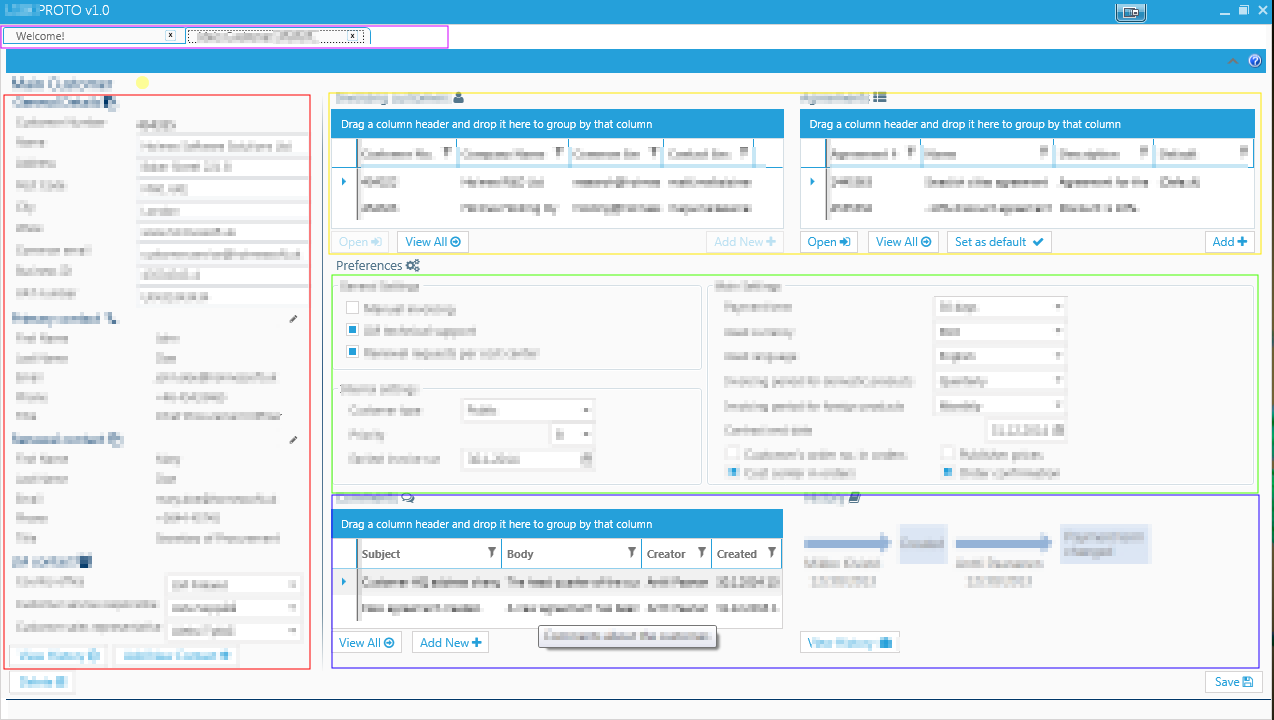
\includegraphics[width=1.3\textwidth]{./images/proto_main.png}
    	   }
  	   \caption{Screenshot of the prototype's ERP component 1.}
	   \label{fig:protooneimg}
\end{figure}

The screenshot \ref{fig:prototwoimg} shows the user interface of the invoicing customer level. The invoicing and delivery customer interfaces don't vary significantly from the main customer interface, which is why there is no separated screenshot of it. There are few small differences though. For example, the pen preferences marked with the dark green color in the contact section. By clicking the pen, a contact dialog opens up. The idea of this dialog is to offer user the possibility to select already existing contact instead of typing all the contact details multiple times. In many occasions, the contact details are the same in different customer levels. Additionally, from the dialog the user can also select the validation period for the contact. 

The closed and open chains next to the preferences, indicates the design idea for the preference inheritance. For example, if a preference is selected at the main customer level and the chain of the same preference is closed in the invoicing customer level, the invoicing customer inherits the selected preference from the main customer. The same procedure functions throughout the whole customer hierarchy, so if some preference is selected in the main customer level and the chains are closed on invoicing and delivery customer levels, the delivery customer inherits the preference from the main customer. The idea behind the design is to point out the inherited preferences, and therefore decrease the users' memory load. It also decrease the users' workload since they don't have to fill out all the details on every level of the hierarchy.   

\begin{figure}[H]
  	\centerline{
    	   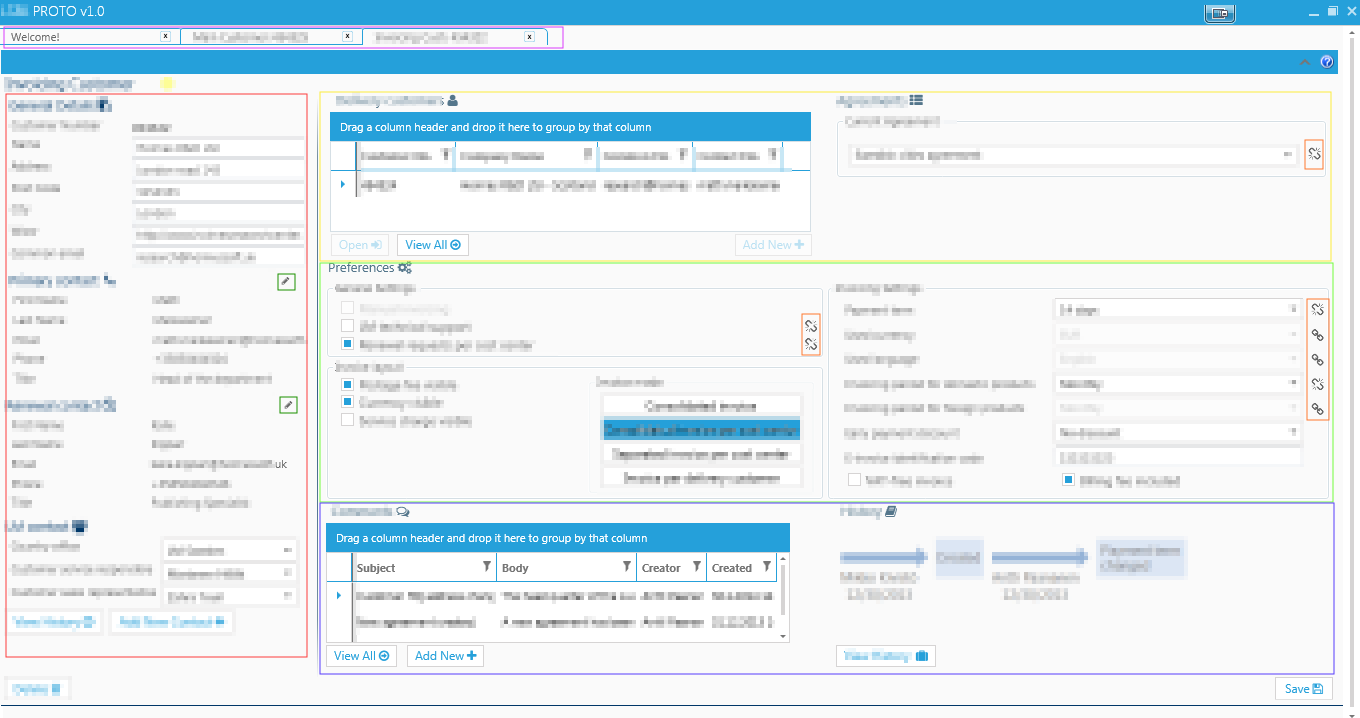
\includegraphics[width=1.3\textwidth]{./images/proto_invoicing.png}
    	   }
  	   \caption{Screenshot of  the prototype's ERP component 2.}
	   \label{fig:prototwoimg}
\end{figure}

There are few differences between the present ERP system and the prototype solution, but many of them are considered confidential. The following paragraph describes some general differences between the two.

Probably the most significant difference between the current system and the prototype solution is that the prototype does not display all the possible settings on every level, but separates the preferences according to the level. Moreover, the prototype functionality to select previous contacts in the contact section, decreases the need to type the same details multiple times, which was not possible in the present system. The tab solution in prototype enables the user to manage multiple different instances of different things simultaneously, which provides a remarkable advantage over the current ERP system. The problems of the inheritance in the current user interface has been prevented with the chain design. Additionally, the existence of the comments and the history sections, separates the present and the new UI versions. Both of them provides valuable information for the user about the customership.

\subsection{Results of the prototype evaluation}

Due to time schedule limitations, only the Swedish users took part in the second evaluation round in addition to the Finnish analyst. This subsection represents the results of the prototype evaluation in chronological order. 

The first evaluation method used to study the usability of the prototype, after the confirmation meeting with the Finnish users, was the Cognitive Walkthrough. The amount of the discovered issues was not remarkably high and only two types of problems were found. The first type of problems was related to the naming conventions. For example, some of the new buttons were labeled in a way which needed clarification. Additionally, some of the labels and settings were named using the corresponding designations in the current system, which still needed some extra specifications. The second type of issues discovered from the prototype was layout problems. It emerged that some critical functions were hidden and were not immediately noticeable , despite their importance for the system. The results of the Cognitive Walkthrough indicates that the usability problems have decreased comparing to the CW implemented during the first evaluation round. However, the results the walkthrough can be misleading because it was accomplished by the developer of the prototype.

The results of the inquiries formed four different categories in affinity diagram and shared 44 different notices. It emerged, that some critical observations stayed unnoticed during the first evaluation round, but appeared in the second, causing problems in the prototype's usability. Additionally, the fully renewed user interface solution entailed some new usability issues. 

The biggest category was named as user interface and functionality problems. The results indicated that the prototype contained some misplaced buttons which should be more hidden or more visible. Moreover, some of the settings should have been available in all the customer levels and some levels were missing a few relevant fields. Even though the prototype introduced some more efficient ways for browsing the data and to browse between the customer levels, some shortcut links were desired to be shown. For example, the open link from the invoicing customer level to the main customer level was missing.  

The second category was named as user interface ideas and it consisted of nine different notices. Many of the notices contained ideas concerning the commenting functionality in the system. For example, most of the users wanted it to be possible to flag or highlight important comments in some way. They also desired additional comment fields to be added to the prototype and the functionality to be able to select on which customer levels the comment will be shown. Additionally, an idea about peek windows for data check were stated. These quick views would provide an outlook to some data behind any link when the mouse is hovered on it. This functionality could be useful, for example, in a case when a customer is making a call and the data were need to be displayed as fast as possible. The category also contained some ideas about how to make entering the customer data easier by utilizing the inheritance between the customer levels. 

The third category contained qualities which were found particularly functional. The results indicate that the layout of the prototype was generally liked. The tab navigation, history and comment sections, advanced search functionality and the chain inheritance design, described in the subsection \ref{sec:demoproto}, were approved by the users. Additionally, the users valued the fact that the hierarchy could not been broken in the prototype version. 

The last category was labeled as 'Needs consideration'. These were the most significant issues found and which requires some design solutions to be implemented in the business process itself. Examples of this kind of issues, could be deciding on the compulsory information required while creating a new customership, or on which level different preferences should be attached in the user interface. Even though the inquiries of the prototype resulted still tens of notices, the usability issues discovered decreased from the current system's 127 to prototype's 44 issues. 

The results of the Interaction Sequence Illustration from the second evaluation round indicates that there are total of nine different interaction stages in the prototype, which is one stage less than in the present system. Because of the lack of the real data, only the maximum amounts of interaction steps could be calculated. The maximum number of possible interaction steps on the main customer level (of the prototype) was 54 steps, which is  29 less than the possible interaction steps of the current system. Moreover, the maximum amount of interaction steps on invoicing customer and delivery customer levels were 47 and 38, comparison to the present system's 83 on all levels. In general, the amount of interaction steps required in customer creation process is evidently decreased with the prototype solution. The decreased amount of interaction steps can decrease the interaction risks and users' workload.

The System Usability Scale score from the second evaluation round with the Swedish users was 74.17, which indicates significant increase in the score comparing to the corresponding score of the current ERP system (50.83). The results strengthens the perception of the earlier results, indicating improvements in the usability of the user interface. 
 
The evaluation of the remote usability logging proved to be impossible because of the lack of real-life usage of the prototype. However, as a result, it seems that it is possible to track the usability and the efficiency of use with the created library. The library was attached to the source code of the prototype and the results were positive. The library functioned correctly, saving all the relevant data of the evaluation sessions. For example, a main customer level creation session, tracked data of the empty main customer object in the beginning of the session and with the data in the end of the session. From the data, it is possible and effortless to analyze that the session in question, was a main customer creation session. Moreover, session's starting time, ending time the user reference were tracked. 

In addition to session data, event usability logging proved to be functional. Details such as event's feature name and object data in the beginning and in the end of the event, were tracked successfully, together with the consumed time and session references. For example, from the main customer creation session, the events of modifying contact data were tracked successfully with the specific details about the contact and the edited features. Basically, all the interaction steps of the events were tracked with the timestamps, user information, feature information and session references.

\begin{figure}[H]
  	\centerline{
    	   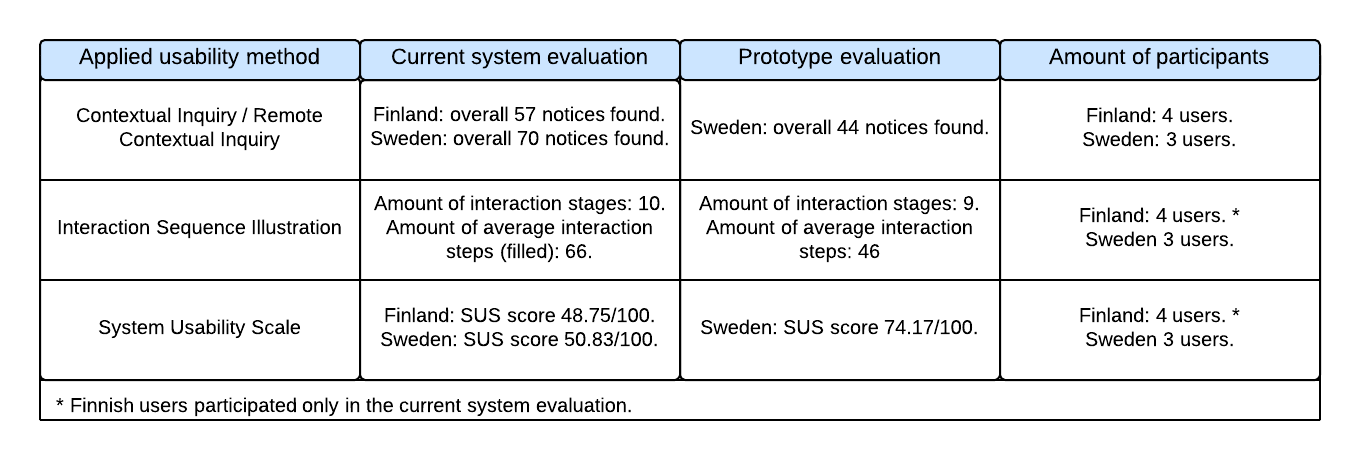
\includegraphics[width=1.3\textwidth]{./images/methodresult.png}
    	   }
  	   \caption{Results of the methods and number of study participants.}
	   \label{fig:methodresults}
\end{figure}

%System Usability Scale
   % -google form
   % \\*
    % -vaihe1: suomessa tulos: 48.75/100
  %   \\*
%	vaihe1: ruotsissa tulos: 50.83/100
%	\\*
  %   -vaihe1: tulos ei välttämättä kerro koko totuutta koska otanta kohtalaisen pienet ja osaamistasot ovat erilaiset. antaa kuitenkin osviittaa.
    % \\*

%vaihe 2. ruotsi 74.17

%    \subsection{Cognitive Walkthrough}
    %- vaihe1. nimeämisessä suuria ongelmia.
 %   -vaihe1.asetuksia ei ole määritelty riittävän tarkoin eri asiakastasoille ==> hierarkia on epäselvä.
 %   -vaihe1.järjestelmä ei tarjoa riittävästi tietoa siitä onko toiminto onnistunut vai ei. 
 %   -vaihe1.järjestelmä saattaa antaa jopa virheellistä tietoa. 
%   -vaihe1. järjestelmä ei huomioi asetusten sisäisiä riippuvuuksia.
 %   -vaihe1.yleisesti järjestelmä ei anna tarpeeksi apua käyttöä ajatellen.
   % -vaihe1.joidenkin asetusten olemassaolo saattaa olla vaikeaa havaita.
   % -vaihe1.ei tarpeeksi hierarkia tietoa.
   % -vaihe1.nimeäminen ei ole yhtenäistä esim. new delivery address vs. new renewal customer.
    
   %    Contextual Inquiry
%	toteutettiin affiniteetti diagrammilla.	
%\\
 %   Onnistui hyvin alun vaikeuksista ja real-life tapausten puutteesta huolimatta.
%	\\
%    vaihe1: suomessa:57 huomiota, ongelmakohtaa,parannusideaa 
  %  \\*
  %  -suomessa:6 kategoriaa
  %  \\*
 %   -ruotsissa:6 kategoriaa mutta erit kuin suomessa
  %  \\*
  %  -vaihe1: ruotsissa: 70 huomiota ongelmakohtaa parannusideaa.
 %   \\*
  %  -ruotsissa focus ajautui hieman eri asioihin.
   % \\*
    %-selkeitä eroja havaittavissa toiminnassa suomen ja ruotsin välillä.

 %analyysi vertaileva ennen ja jälkeen + vanhaan aineistoon vedoten.
%\\*
     
 %    \subsection{Interaction Sequence Illustration}
    % 	  -interaktioiden ajallinen mittaaminen ei onnistu
%	  \\*
%	  -interaktioiden määrä vaihtelee riippuen tilanteesta.aiheutti hankaluuksia, joten otettu keskiarvo ja kyselty käyttäjiltä mitä nämä tavallisesti tekisivät.
%	  \\*
%	  -mitkä ovat interaktio stepit ja staget.
%	  \\*
%	  -vaihe1: interaktio katsottu videolta ja laskelmat tehty olemassa oleviin asiakkuuksiin syötettyjen tietoihin perustuen. 50 satunnaisotanta antanee kohtalaisen selkeän kuvan siitä kuinka paljon prosessi vaatii interaktioita.
%	  \\*
%	  -vaihe 1: järjestelmä antaa periaatteessa mahdollisuuden täyttää 83 kenttää per asiakastyyppi + aloitus stepit -> käytännössä näin ei kuitenkaan ole.
%	  \\*
%	  -vaihe1:sopimusasiakkaalla 50 satunnaisotannan avg. steppien määrä on 23, pienin 9 ja suurin 35 (laskettu tietojen syötöstä  tallenna-klikkaukseen.)
%	  \\*
%	  -vaihe1:laskutusasiakkalla 50 satunnaisotannan avg. steppien määrä on 14,48, pienin 9 ja suurin 22 (laskettu lisää laskutusasiakas -painikkeen klikkauksesta tallentamiseen)
%	  \\*
%	  -vaihe1:toimitusasiakkaalla 50 satunnaisotannan avg. steppien määrä on 12,94, pienin 11 ja suurin 18 (laskettu lisää toimitusasiakas -painikkeen klikkauksesta tallentamiseen)
%	  \\*
%	  -vaihe1:uudistusasiakkaalla 50 satunnaisotannan avg. steppien määrä on 15,66 pienin 11 ja suurin 24 (laskettu lisää uudistusosoite -painikkeen klikkauksesta tallentamiseen). myös laskutusasiakas voi olla uudistusasiakas, mikä voi vääristää tulosta hieman.
%	  \\*
%	  -vaihe1:yhteensä asiakasinteraktioiden avgt on 66,08 steppiä. tähän tulee kuitenkin lisätä vielä libsysin käynnistykseen liittyvät stepit.
%	  \\*
%	  -10 stagea havaittu
%	  \\*
%	  -step-by-step kuvaus jätetty pois
%	  \\*
%	  -luvuissa ei mukana alennusten lisäystä, e-access detailsien lisäystä, eikä cost centereiden lisäystä. 
%	  \\*
     







\section{Functionality of the methods in the context of study}
The applied methods were chosen according to their practicality and suitability to the study context (see chapter \ref{chapter:methods}). The suitability to study context referred to the methods' adaptability to the human-centered design activities and thereby possibly to the subscriber company's software development process. However, the evaluations and the results indicate that not all of the applied methods were suitable for this specific case. On the other hand, a few of the methods generated significant amount of beneficial usability data. 

The most successful method was Contextual Inquiry, resulting specific and easily exploitable data. Applying the method remotely (Remote Contextual Inquiry) didn't have any significant affect on the efficiency of the evaluation. This may be derived from the in-house development approach, which made it easier to interview the users in a natural and comfortable manner. Additionally, the remote inquiries were planned carefully and the technological problems were minimized. However, it is possible that Remote Contextual Inquiry wouldn't create that great benefit in comparison to the traditional Contextual Inquiry, in some other context of study. Inquiries were applied in three stages of the human-centered design (Understand and specify the context of use, specify the user requirements and evaluate the designs against requirements) and produced beneficial results from every one of them. Additionally, the methods gave a great insight into the cultural differences between Finnish and Swedish country offices.

Interaction Sequence Illustration was also applied in three human-centered design stages. The method produced a good results giving a deep understanding about the different stages of the examined process. However, because of the varying structure of the customer creation process, the method could not be utilized as widely as normally. Moreover, considering the possible future iterations, the effectiveness of the ISI method will slowly fade away, because no significant differences in the process itself will emerge as the development continues. This is why ISI is more functional in a situation where the object or the process of study is static, and when the context of use need to be fully understood for the first time. 

The Cognitive Walktrough was applied in two stages of the human-centered design: specifying the user requirements and evaluating the designs against the requirements. In the study, CW was functional in first of them. The inspection of the current system produced results which were not identified with the other methods. However, the inspection of the prototype, and therefore the stage of evaluating the design against the requirements, didn't yield to any great results. A most remarkable difference between the two inspections were that the analyst was not participated in the development of the current system, but was developing the prototype. This indicates, that if the CW will be applied in a development process, the analyst shouldn't be also a developer of the system.  

The System Usability Scale turned out to be practical and quick way of perceiving the level of user satisfaction and the UX. It also provides a great insight into the differences between different cultures. However, in the study, too small amount of data was gathered. In order to fully benefit from the method and in order to gain reliable usability data, more people are required to answer the questionnaire. However, gathering more data can be challenging in a small or middle-sized companies. Moreover, previous data would provide a good baseline for the next evaluations, which would make the results more valuable to the company. Still, the method provides a good general view of the user satisfaction. The produced benefits seem to overrule the effort of implementation in the context of in-house software development. The method is applied in three stages of the human-centered design. It is used to understand and specify the context of use, or in this case the level of user satisfaction of the current system. It is also utilized to support the specification of the user requirements (by stating the user satisfaction) and to evaluate the designs against the requirements. The method indicates the differences in user satisfaction between the development iterations. Consequently, it is beneficial for long-term in-house software development . Additionally, it is relatively effortless to gather data with the method, because the response rate is significantly high when the study is accomplished internally.

Remote usability logging is applied in one stage of the human-centered design. It was supposed to use to evaluate the designs against the requirement, but because of the lack of previous data, the evaluation became considerably pointless. However, the created library could be used in the future iterations, when there would be comparable data available. As a conclusion, the method will bring value only when the data from at least two iterations are available for comparison. Nevertheless, after two evaluations, the method provides specified data about the usage of the system.
      


      
%-if a process need to be understood or the aim is for example to minimize the interaction steps  it might be beneficial to utilize ISI in the beginning of the new process. ISI could be a good way to document static business processes. in a long run not good. not suitable for %iterative development. if utilized, need to be separated per process which might be difficult in some cases. also, might not be efficient enough. 
%- sus needs more data but is quite easy to implement and gives a good overview of the system in general. in the case of erp system could be also utilized per process or per user role which might be difficult but useful.
%-cognitive walktrough could be utilized if there would be an analyst outside the company, which might be difficult. in general the results were not that magnificent.
%-remote usability logging would be could for iterative development and when the library has been already implemented there should be no reason for not to attach it as a part of the development. needs more data and someone to analyze the data but in the end quite good option.




    
   % -VARSINAISET TULOKSET!!!!!!!!!!!!!!!!!!!!!!!!!!!!!!!!!1
%    -CI:n ja RCI:n välillä ei huomattavia eroja, jos haastattelut on suunniteltu/toteutettu hyvin ja kaikki toimii. Saattaisi olla hyvin eri asia jos kyseessä olisi ulkopuolinen käyttäjä.
%    -menetelmillä saatiin hyvin esille ruotsin ja suomen erilaisia tarpeita. esim. tavoissa toimia on eroja. but still the differences between two countries are relatively small.
%  -While writing the thesis, contextual inquiry used as part of requirement definition process of the process..

  %-*koska toisellakin kierroksella löytyi ongelmia, voidaan todeta että CI toimii iteratiivisessa kehityksessä,

%  -lisää sus dataa tarvitaan. 


%  -remote logging tarvitsee paljon dataa analyysiä varten.

 %% -cw ei ole hyvä muutosten testaamiseen, ainakaan jos testaaja on sama kuin kehittäjä.
%- vielä löytyi ongelmia, implicates that iterations are needed. silti huomattavaa parannusta huomattavissa
%- applied process can improve the umm level and thereby the cmmi level.,

%-after the study, ci and remote usability logging have been utilized. 



%\begin{itemize}
%\item \textbf{\emph{How usability methods can help to identify critical disparities in the usage of a system?}}

%Understanding the differences in the system's usage between individuals and cultural manners can help to understand and deploy the best practices throughout the organization, identify issues in the system, and thereby increase efficiency.

%\item \textbf{\emph{How applying the human-centered design can improve in-house software development process?}}

%Can the in-house software development process benefit from the principles of human-centered design.

%\item \textbf{\emph{What usability methods can be practically joined with the  software development process of an ERP system?}}

%Finding practical and efficient usability methods to be joined with the software development process, can improve the quality and efficiency of the end product, and also raise process' maturity level.

%\end{itemize}


\section{Implementation guidelines}
\label{sec:implementationguidelines}

The experiences of implementing usability evaluations as a part of in-house software development process were highly positive. The users as a part of the development organization provides great advantages over the development for external users. The users can be approached easily and therefore the feedback and data can be gathered without significant effort. However, there are some matters to be considered before the implementation of the applied human-centered design. 

Even though the in-house software development benefits greatly from the contribution of internal users, the users might lack of fresh ideas. This is why it is important not to forget to think outside the box, and not to comply only with the old practices.  
It is also advisable to remember that the methods implemented in the study might not be suitable for all companies. Every company applying the human-centered design should select the methods most suitable for their specific needs. 

It is crucial not to forget the other aspects of the software development process. The applied human-centered design can assist a company to improve their Usability Maturity Model level and therefore to improve the Capability Maturity Model Integration level. An improvement in both of the models represents improvements in in-house software development process. However, in order to improve the software development as a whole, several other aspects should be considered as well and the higher levels of the two maturity models should be pursued systematically.

In general, the evaluations could be implemented more efficiently and lighter way that in the thesis work. In the case of the subscriber company, the inquiries and the SUS questionnaire should be applied in every country office in order to find more detailed information about the cultural differences and to gather more reliable usability data. The remote usability logging should be utilized, from the beginning of the new ERP system development, meaning that the library should be referenced in the code in an iterative manner. This way the implications of changes could be tracked efficiently and the functionality of the method could be defined in more detail. Additionally, the prototype designs created in the later stages of the development or from the other processes (than customer management), can be implemented in a lower level of detail. For example mock-ups and paper prototyping could be applied to accomplish the same results as with a high-fidelity prototype, but only faster. In general, the usability evaluations and human-centered design activities should be kept as agile and efficient as possible, in order to create a real value for the in-house software development process.  
 
 % - jalkauttaa kaikkialle.
%-applied human-centered design process on hyvä in-house software developmentiin mutta kaikkien yritysten tulisi käyttää juuri itselleen sopivia menetelmiä, eli valitsemamme menetelmät eivät toimi kaikille.
%- applied process can improve the umm level and thereby the cmmi level.,
%-voidaan toteuttaa tehokkaammin ja yksinkertaisemmin ja säästeliäämmin.
%-umm levels should be achieved systematically.
%-not necessary to implement so high details prototypes. mockups could be enough if development is iterative.

%-The experiences of implementing usability evaluations as a part of in-house software development were highly positive. The cooperation was remarkably effortless because of the users were part of the developing organization.  
%-pitää muistaa että sisäisesti toteutettavissa ohjelmissa saattaa puuttua fresh opinion
%
%    -Should these methods be implemented as a part of the process or not.
%-luultavasti helpompaa kuin ulkoisille asiakkaille

%-jokaisen yrityksen tulee valita tarpeisiinsa sopivat menetelmät, kaikki ei toimi kaikille
%recommendations about the methods: kolme menetelmääö	
%
%
%-if utilizing cw do not use same persons to develop and inspect.
%
%
%-yleisesti in-house helpottaa evaluointia


%When you use \texttt{pdflatex} to render your thesis, you can include PDF images
%directly, as shown by Figure~\ref{fig:indica_model} below.

%\begin{figure}[ht]
%  \begin{center}
%    \includegraphics[width=\textwidth]{example_indica_model.pdf}
%    \caption{The INDICA two-layered value chain model.}
%    \label{fig:indica_model}
%  \end{center}
%\end{figure}

%You can also include JPEG or PNG files, as shown by Figure~\ref{fig:eeyore}.

%\begin{figure}[ht]
%  \begin{center}
%    \includegraphics[width=9cm]{example_ihaa.jpg}
%    \caption{Eeyore, or Ihaa, a very sad donkey.}
%    \label{fig:eeyore}
%  \end{center}
%\end{figure}


%If you have PS or EPS files, you can use the tools \texttt{ps2pdf} or
%\texttt{epspdf} to convert your PS and EPS files to PDF\@.

% Comment: If your sentence ends in a capital letter, like here, you should
% write \@ before the period; otherwise LaTeX will assume that this is not
% really an end of the sentence and will not put a large enough space after the
% period. That is, LaTeX assumes that you are (for example), enumerating using
% capital roman numerals, like I. do something, II. do something else. In this
% case, the periods do not end the sentence.

% Similarly, if you do need a normal space after a period (instead of
% the longer sentence separator), use \  (backslash and space) after the
% period. Like so: a.\ first item, b.\ second item.


%WYSIWYG vector editor that allows you to save directly to PDF\@.

%Excel to PDF format, and then add them; or use \texttt{gnuplot}, which can
%something like \texttt{set term pdf \ldots}.


%rather steep learning curve. Locate the manual (\texttt{pgfmanual.pdf}) from
%graphics is shown in Figure~\ref{fig:page-merge}.

%\begin{figure}[ht]
%  \begin{center}
%    \input{example_page-merge.tex}
%    \caption{Example of a multiversion database page merge. This figure has
%    been taken from the PhD thesis of Haapasalo~\citep{HaapasaloThesis}.}
%    \label{fig:page-merge}
%  \end{center}
%\end{figure}


% These definitions are only used in the example images; you will not
% need them for your thesis...
%\newlength{\graphdotsize}
%\setlength{\graphdotsize}{1.7pt}
%\newlength{\graphgridsize}
%\setlength{\graphgridsize}{1.2em}
%\begin{figure}[ht]
%\begin{center}
%\subfigure[Examples of obstruction graphs for the Ferry Problem]{
%  \input{example_obstruction-grouped.tex}
%}
%\subfigure[Examples of star graphs]{
%  \input{example_general-star-graphs.tex}
%}
%\caption{Examples of graphs draw with TikZ. These figures have been taken from a
%course report for the graph theory course~\citep{FerryProblem}.}
%\label{fig:tikz-examples}
%\end{center}
%\end{figure}



% \chapter{Methods}
\label{chapter:methods}

You have now stated your problem, and you are ready to do something
about it!  \emph{How} are you going to do that? What methods do you
use?  You also need to review existing literature to justify your
choices, meaning that why you have chosen the method to be applied in
your work.

% An example of a traditional LaTeX table
% ------------------------------------------------------------------
% A note on underfull/overfull table cells and tables:
% ------------------------------------------------------------------
% In professional typography, the width of the text in a page is always a lot
% less than the width of the page. If you are accustomed to the (too wide) text
% areas used in Microsoft Word's standard documents, the width of the text in
% this thesis layout may suprise you. However, text in a book needs wide
% margins. Narrow text is easier to read and looks nicer. Longer lines are 
% hard to read, because the start of the next line is harder to locate when
% moving from line to the next. 
% However, tables that are in the middle of the text often would require a wider
% area. By default, LaTeX will complain if you create too wide tables with
% ``overfull'' error messages, and the table will not be positioned properly
% (not centered). If at all possible, try to make the table narrow enough so
% that it fits to the same space as the text (total width = \textwidth).
% If you do need more space, you can either
% 1) ignore the LaTeX warnings 
% 2) use the textpos-package to manually position the table (read the package
%    documentation)
% 3) if you have the table as a PDF document (of correct size, A4), you can use
%    the pdfpages package to include the page. This overrides the margin
%    settings for this page and LaTeX will not complain.
% ------------------------------------------------------------------
% Another note:
% ------------------------------------------------------------------
% If your table fits to \textwidth, but the cells are so narrow that the text
% in p{..}-formatted cells does not flow nicely (you get underfull warnings 
% because LaTeX tries to justify the text in the cells) you can manually set
% the text to unjustified by using the \raggedright command for each cell 
% that you do not want to be justified (see the example below). \raggedleft 
% is also possible, of course...
% ------------------------------------------------------------------
% If you need to have linefeeds (\\) inside a cell, you must create a new
% paragraph-formatting environment inside the cell. Most common ones are 
% the minipage-environment and the \parbox command (see LaTeX documentation
% for details; or just google for ``LaTeX minipage'' and ``LaTeX parbox'').
\begin{table}
\begin{tabular}{|p{2cm}|p{3.8cm}|p{4.5cm}|p{1.1cm}|} 
% Alignment of sells: l=left, c=center, r=right. 
% If you want wrapping lines, use p{width} exact cell widths.
% If you want vertical lines between columns, write | above between the letters
% Horizontal lines are generated with the \hline command:
\hline % The line on top of the table
\textbf{Code} & \textbf{Name} & \textbf{Methods} & \textbf{Area} \\ 
\hline 
% Place a & between the columns
% In the end of the line, use two backslashes \\ to break the line,
% then place a \hline to make a horizontal line below the row 
T-110.6130 & Systems Engineering for Data Communications
    Software & \raggedright Computer simulations, mathematical modeling,
  experimental research, data analysis, and network service business
  research methods, (agile method) & T-110 \\ 
\hline
\multicolumn{2}{|p{6.25cm}|}{Mat-2.3170 Simulation (here is an example of
 multicolumn for tables)}& Details of how to build simulations & T-110 \\
% The multicolumn command takes the following 3 arguments: 
% the number of cells to merge, the cell formatting for the new cell, and the
% contents of the cell
\hline
S-38.3184 & Network Traffic Measurements and Analysis 
& \raggedright How to measure and analyse network
  traffic & T-110 \\ \hline
\end{tabular} % for really simple tables, you can just use tabular
% You can place the caption either below (like here) or above the table
\caption{Research methodology courses}
% Place the label just after the caption to make the link work
\label{table:courses}
\end{table} % table makes a floating object with a title

If you have not yet done any (real) metholodogical courses (but chosen
introduction courses of different areas that are listed in the
methodological courses list), now is the time to do so or at least
check through material of suitable methodological courses. Good
methodologial courses that consentrates especially to methods are
presented in Table~\ref{table:courses}. Remember to explain the
content of the tables (as with figures). In the table, the last column
gives the research area where the methods are often used. Here we used
table to give an example of tables. Abbreviations and Acronyms is also
a long table. The difference is that longtables can continue to next
page.




% An example of a traditional LaTeX table
% ------------------------------------------------------------------
% A note on underfull/overfull table cells and tables:
% ------------------------------------------------------------------
% In professional typography, the width of the text in a page is always a lot
% less than the width of the page. If you are accustomed to the (too wide) text
% areas used in Microsoft Word's standard documents, the width of the text in
% this thesis layout may suprise you. However, text in a book needs wide
% margins. Narrow text is easier to read and looks nicer. Longer lines are
% hard to read, because the start of the next line is harder to locate when
% moving from line to the next.
% However, tables that are in the middle of the text often would require a wider
% area. By default, LaTeX will complain if you create too wide tables with
% ``overfull'' error messages, and the table will not be positioned properly
% (not centered). If at all possible, try to make the table narrow enough so
% that it fits to the same space as the text (total width = \textwidth).
% If you do need more space, you can either
% 1) ignore the LaTeX warnings
% 2) use the textpos-package to manually position the table (read the package
%    documentation)
% 3) if you have the table as a PDF document (of correct size, A4), you can use
%    the pdfpages package to include the page. This overrides the margin
%    settings for this page and LaTeX will not complain.
% ------------------------------------------------------------------
% Another note:
% ------------------------------------------------------------------
% If your table fits to \textwidth, but the cells are so narrow that the text
% in p{..}-formatted cells does not flow nicely (you get underfull warnings
% because LaTeX tries to justify the text in the cells) you can manually set
% the text to unjustified by using the \raggedright command for each cell
% that you do not want to be justified (see the example below). \raggedleft
% is also possible, of course...
% ------------------------------------------------------------------
% If you need to have linefeeds (\\) inside a cell, you must create a new
% paragraph-formatting environment inside the cell. Most common ones are
% the minipage-environment and the \parbox command (see LaTeX documentation
% for details; or just google for ``LaTeX minipage'' and ``LaTeX parbox'').
%\begin{table}
%\begin{tabular}{|p{2cm}|p{3.8cm}|p{4.5cm}|p{1.1cm}|}
% Alignment of sells: l=left, c=center, r=right.
% If you want wrapping lines, use p{width} exact cell widths.
% If you want vertical lines between columns, write | above between the letters
% Horizontal lines are generated with the \hline command:
%\hline % The line on top of the table
%\textbf{Code} & \textbf{Name} & \textbf{Methods} & \textbf{Area} \\
%\hline
% Place a & between the columns
% In the end of the line, use two backslashes \\ to break the line,
% then place a \hline to make a horizontal line below the row

%    Software & \raggedright Computer simulations, mathematical modeling,

%\hline
%\multicolumn{2}{|p{6.25cm}|}{Mat-2.3170 Simulation (here is an example of
% multicolumn for tables)}& Details of how to build simulations & T-110 \\
% The multicolumn command takes the following 3 arguments:
% the number of cells to merge, the cell formatting for the new cell, and the
% contents of the cell
%\hline
%S-38.3184 & Network Traffic Measurements and Analysis
%& \raggedright How to measure and analyse network
%  traffic & T-110 \\ \hline
%\end{tabular} % for really simple tables, you can just use tabular
% You can place the caption either below (like here) or above the table
%\caption{Research methodology courses}
% Place the label just after the caption to make the link work
%\label{table:courses}
%\end{table} % table makes a floating object with a title



% \chapter{Implementation}
\label{chapter:implementation}

You have now explained how you are going to tackle your problem. 
Go do that now! Come back when the problem is solved!

Now, how did you solve the problem? 
Explain how you implemented your solution, be it a software component, a
custom-made FPGA, a fried jelly bean, or whatever.
Describe the problems you encountered with your implementation work.




% \chapter{Evaluation}
\label{chapter:evaluation}

You have done your work, but that's\footnote{By the way, do \emph{not} use
shorthands like this in your text! It is not professional! Always write out all
the words: ``that is''.} not enough. 

You also need to evaluate how well your implementation works.  The
nature of the evaluation depends on your problem, your method, and
your implementation that are all described in the thesis before this
chapter.  If you have created a program for exact-text matching, then
you measure how long it takes for your implementation to search for
different patterns, and compare it against the implementation that was
used before.  If you have designed a process for managing software
projects, you perhaps interview people working with a waterfall-style
management process, have them adapt your management process, and
interview them again after they have worked with your process for some
time. See what's changed.

The important thing is that you can evaluate your success somehow.
Remember that you do not have to succeed in making something spectacular; a
total implementation failure may still give grounds for a very good master's
thesis---if you can analyze what went wrong and what should have been done.

 




%You have done your work, but that's\footnote{By the way, do \emph{not} use







% \chapter{Discussion}
\label{chapter:discussion}

At this point, you will have some insightful thoughts on your implementation
and you may have ideas on what could be done in the future. 
This chapter is a good place to discuss your thesis as a whole and to show your
professor that you have really understood some non-trivial aspects of the
methods you used\ldots



\chapter{Conclusions and discussion}
\label{chapter:conclusion}

In this research study, the aim was to examine the subscriber company's customer management process, or more precisely, customer creation process,  in their current Enterprise Resource Planning (ERP) system. The aim was also to discover its usability issues and define user requirements for the future system. However, the biggest goal of the study was to find out if the organization's in-house software development process can be improved by applying human-centered design activities. This chapter discusses about the conclusions of the study and about the future work to be conducted. The chapter also answers the research questions.



\section{Answers to the research questions}

The study and the results show, that the applied methods can help to identify critical disparities in the usage of a system. The inquiries revealed most of the disparities, but it is likely that in a wide timespan for example System Usability Scale and remote usability logging would reveal more and more differences between the system usage in different country offices. Even though the cultural differences between Finland and Sweden are not particularly significant, the two implemented evaluation rounds exposed multiple differences in the system usage and in the work process itself. It is highly likely, that if more diverse cultures would be joined to the study, the results would even richer. The Cognitive Walktrough and Interaction Sequence Illustration did not expose any remarkable disparities between the cultures. 

According to the results, an in-house software development process can benefit from applying the human-centered design. The results indicate, that the usability did improve with the iterative development and that the software development process itself has improved by applying the human-centered design. The improvement is based on increase in the company's Usability Maturity Model level. Evidently, the company's UMM level has increased from level A to the level B. Clearly, level A was a condition for this study, meaning that the organization identified the need for improvement in the system's quality of use. The implemented evaluations raised the UMM level to A2, by describing a number of usability activities to be performed and by gathering user requirements. 

The actions the company have taken (not related to the study) indicates that the UMM level has been reached level B. For example, the evaluation of the other ERP processes (in addition to the customer management) have been proposed to be attached to the software development of the new system. This proposition is made due to encouraging amount of requirements gathered from the customer management process. In practice, the company wants to utilize inquiries in the requirement definition process and the remote usability logging library has already been applied in another project. Thereby, it can be stated that the quality of use is considered as an important attribute in the development. In general, the transition from the level A to level B designates for cultural change in the company, from experience based to more user-centric development. 

The increase of UMM level also affects on the company's Capability Maturity Model Integration process areas. For example, usability evaluations have an affect on level three and its process areas, such as requirements development (by providing usability related requirements), risk management (by providing more usable and efficient solutions) and validation (by providing usability validations). All the changes in the company's maturity levels show that by applying the human-centered actions, the in-house software development process can be improved.

%-What usability methods can be practically joined with the in-house software development process of an ERP system?
The results indicate that the Contextual Inquiry and Remote Contextual Inquiry methods, can be practically joined with the in-house software development process of an ERP system. This argument is based on the qualitative outcomes of applying the methods. The inquiries are particularly suitable for studying big systems like an ERP, because it can be applied to each of the detected processes, and thereby to gain understanding about the entire system's context of use. Additionally, the inquiries fit well in an iterative process. The second evaluation round produced significant amount of usability issues, even if the prototype was designed by applying the information gathered from the first evaluation round. This implicates, that the iterative utilization of the inquiries should be considered. 

The inquiries are remarkably easy to attach to in-house software development process since the users are easily available for the evaluations, and the methods are in general relatively effortless to apply. Moreover, applying the inquiries is very cost-efficient way to gather usability data. The Remote Contextual Inquiry can be utilized to gather cultural related usability data with low cost, which makes it particularly considerable and practical option for in-house software development context. Moreover, the affinity diagram is a practical solution for data display and categorization. It enables the identification of critical usability themes and issues, quickly and efficiently.   

Applying Interaction Sequence Illustration should be considered if a process is need to be understood thoroughly, or the aim is to make the user interface as straightforward as possible, and to minimize the interaction steps. The ISI is particularly beneficial if the studied process is not perceived thoroughly. Thereby, it could be applied to document the business processes. However, if the process is not static and the usage of the system varies constantly, the utilization of the method becomes redundant. The process evaluation with the ISI can be beneficial in the beginning of the iterative development process, but does not bring any extra value in a long run. Due to enormous scope of the ERP system, the method should be utilized per business process. However, in some occasions, defining a business process might be difficult or even impossible to accomplish. Because of these reasons, the Interaction Sequence Illustration is not necessarily the most adaptive evaluation method to be attached to the in-house software development process.

The System Usability Scale does not bring value in a short timespan. It requires previous data for interpretations to be reliable enough for the development purposes. Due to wide scope and multiple processes of an ERP system, the SUS could be implemented per process or per specified user role. Divided examination could enable the detection of the most problematic processes or user interface sections. Additionally, SUS is extremely easy to implement as a part of the in-house software development process and in a long timespan, offers a good overview of the system's usability and user satisfaction. 

The results of the Cognitive Walktrough evaluations were not particularly exceptional. Arguably, the reason for unsatisfactory outcome from the second evaluation round is due to the analyst being also the developer of the prototype. However, the results from the first evaluation round did not yield anything remarkable either, even if the analyst was not a developer of the system. In order to gain any essential information by applying the CW, the analyst of the system should not be a member of the software development team, or rather, not even an employee of the company. Considering the in-house aspect of the software development, exploiting an external analyst might not be convenient or even advisable. Due to these reasons, the Cognitive Walktrough is not probably the most functional method to be attached to in-house software development process of an ERP system. 

The remote usability logging did not produce any analyzable data, which is why the practicality and utility of the method is infeasible to estimate. The method needs to be attached to the production environment in order to gather beneficial data, which also requires analysis. Only then, the functionality of the method as a part of the in-house software development process can  be assessed. However, the designed remote logging library is effortless to attach to any process or user interface solution, and significant amount of data can be acquired automatically. The in-house approach also enables the data acquisition without any privacy or legislation issues. Because of its simplicity, remote usability logging can be practically joined with the development process of an  ERP system. Still, longer iterative usability tracking is required to confirm the usefulness of the method.

As a summary, the recommended usability methods for the subscriber company's applied human-centered design process would be the following: Contextual Inquiry and Remote Contextual Inquiry to understand the context of use, discover cultural differences in usage, and to define and redefine the user requirements. System Usability Scale to get the subjective ratings about the usability, and an overview about the user satisfaction. Remote usability logging to gather hidden usability, performance and usage data to be exploited in the software development. 

In addition to the recommended methods, the subscriber company could seek for new methods to support the applied human-centered design as a part of the in-house software development and in order to find the best and most suitable combination of methods.
 


\section{Conclusions of the study}
The study consisted of several stages. Firstly, literature about the topic was examined and a set of usability methods were adapted into different human-centered design activities. Secondly, the current ERP system was studied and evaluated by applying the set of methods, and by analyzing the usability data. Thirdly, a prototype was created according to the findings from the evaluations, and then the prototype was evaluated again with a set of usability methods. The practical actions of the study were implemented in an iterative manner and according to the applied human-centered design activities.

The results were versatile and consisted of usability issues, user requirements, user interface mock-ups, user interface prototype and remote usability logging code library. The discovered usability issues concerned the current ERP system of the subscriber company and  the prototype. The biggest categories of usability issues were related to user interface, naming conventions, the company's customer hierarchy and functionality problems. Most of the usability issues lead then to user requirements. The user interface mock-ups and the prototype were designed to lead the conversation and the development of the future system, and to gather feedback from some of the design solutions. The source code library for remote usability logging was developed to gather usability data in the future development process.  

The results also included recommendations of the methods that could be utilized by subscriber company to improve their software development process. It emerged that some of the applied usability methods were not suitable for the studied business process and for the iterative in-house software development of an ERP system. Eventually, four, out of six applied methods (Contextual Inquiry, Remote Contextual Inquiry, remote usability logging, System Usability Scale), were proved to be most appropriate or promising to be applied on the subscriber company's software development process. These methods identified the most critical cultural disparities in the usage of the current system as well.

To summarize, the results indicate that the in-house software development process can be improved by applying human-centered activities, but the level of improvement depends on the project, selected methods and previous maturity levels of the company. Additionally, the fact that the results cannot be collected all at once, implies the need for iterative development. Moreover, applying the human-centered activities can lead to the achievement of higher Usability Maturity Model levels and Capability Maturity Model Integration levels, and thereby, the in-house software development process can be improved.   

The study process was not without problems. Initially, the plan was to measure and compare the time consumption of customer creation process, when accomplished with the current ERP system and the prototype. The plan proved to be infeasible during the early stages of the study. The dynamic nature of the process was the reason why the time consumption of the process could not have been measured. Moreover, the usability evaluation methods for the applied human-centered design process should have been selected more carefully. 
Some of the evaluation methods emerged to be unsuitable for studying the process. For example, the Cognitive Walktrough required external resources to be beneficial enough, and the calculation of the interaction steps in Interaction Sequence Illustration did not succeed, once again, due to dynamic  nature of the process. In addition, the use of predefined tasks in the evaluation, proved to be problematic because the users were executing the tasks too roughly in order to be able to gather any useful data. This is why a compromise solution for the analysis was required, and the interaction steps were calculated from the previous data of the current system. 

The extent of the process, in comparison to the schedule of the study, caused difficulties to the prototype development, and all the dummy features were not perfected. In addition to the restrictive schedule, a few significant and undefined sections of the future business process lead into challenges in the user interface design, and could not be implemented precisely. Moreover, the application of the remote usability logging library did not bring any significant results. This was caused by the lack of real-life cases. However, the problem was known already in the beginning of the study.
%-alunperin ajatuksena oli mitata myös prosessin suorittamista ajallisesti vanhalla ja uudella käyttöliittymällä mutta sekin osoittautui mahdottomaksi, koska tilanteet vaihtelivat niin paljon, ja oikeaa tarvetta ei ollut tarpeeksi.
%-jotkin menetelmät eivät toimineet niinkuin niiden oli tarkoitus (CW ja ISI). ISI:n käyttö osoittautui mahdottomaksi, joten kompromissiratkaisu.
%-ennaltamääriteltyjen tehtävien suorittaminen ISI-tarkoitukseen osoittautui haasteelliseksi, käyttäjät tekivät tehtävät liian summittaisesti.
%-vaikeuksia aiheutti prosessi laajuus suhteessa käytettävissä olevaan aikaan jolloin käyttöliittymäkehitys oli vaikeaa
%-remote usability logging dataa ei saatu, jotta olisi voitu analysoida, tämä oli toisaalta tiedossa jo tutkimuksen alussa.
%-joidenkin laajojen osa-alueiden määrittelyjen puute tulevaan järjestelmään aiheutti vaikeuksia prototyypin luomiseen ja sitä kautta koko tutkimukseen. 
%-menetelmien valinnassa olisi voinut käyttää kuitenkin harkintaa.
The reliability of the study is highly dependent on the results gained by applying the usability methods on the current system and the prototype. The reliability of the results, on the other hand, can be assessed in two ways: method-by-method or as a whole. The reliability of the SUS is arguable because the amount of participants was not particularly high. However, the SUS score of the two evaluation rounds (evaluating the current ERP and the prototype) were significantly unequal, which indicates that the results give, at least, an overview about the state of the user satisfaction and user experience. 

There is no guarantee on the reliability of the remote usability logging data, because there is hardly few available, and the method requires an authentic environment. Nevertheless, the created library functions well, and the sample data corresponds to the actions taken in the user interface. The results of the Contextual Inquiry and the Remote Contextual Inquiry are reliable. The hypothesis is supported by the fact that the results of the last inquiries of both evaluation rounds started to recur and no new discoveries were made during the las inquiries. 

The reliability is also reduced because the evaluations were implemented only in two countries, due to time schedule limitations. Extending the research to multiple country offices would have produced more data and probably would have strengthen the earlier findings. Additionally, proofs from a longer time periods are required to ensure that the company's UMM and CMMI levels have been truly increased.

%miksi luotettava ja miksi epäluotettava
%-SUS:ssa liian vähän dataa.. liian vähän henkilöitä, mutta antoi silti suuntaviivat.
%-remote usability loggingista ei juuri lainkaan dataa,vaatii aidon ympäristön, mutta toimi hyvin.
%-kulttuurieroja olisi pitänyt pystyä etsimään useammista maakonttoreista, mutta aikataulullisesti mahdotonta. 
%-inquiry tulokset vaikuttavat luotettavilta, sillä viimeisissä haastatteluissa ei ilmennyt enää juurikaan uutta tietoa.
%-vaikka puutteita datassa ja tutkimuksen laajuudessa, yleisesti kaikkien menetelmien tuottamaa yleisnäkemystä voitaneen pitää luotettavana.

Overall, of the research study was successful and it produced desired results. Despite the solidity issues of single evaluations and some shortages in data, the results can be relied on in a general level and the overview of the results indicate improvements in the usability of the system and in the in-house software development process.

%-tutkimus kootaan yhteen ja vedetään päätelmät tuloksiin perustuen. 
%arvioidaan tutkimuksen onnistumista.
%-in-house software development process  can be improved with human-centered activities, how much and with what methods, depends on company and project and the maturity levels of the company.
%-miksi tulokset eivät luotettavia ja miksi taas ovat.
%-important to find suitable usability methods for the de facto company.
%-prototype creation and remote usability logging library went okay. maybe prototype should have been even more detailed, or just mock-up.
%-more data should have been collected and selection of methods should have been considered more carefully.
%-results were promising. especially inquiries gave good results... 
%-iterative development is a must, considering the results (after first evaluation, still a lot of problems were found.)

%jos käytetään hcd:tä ja menetelmiä voidaan päästä eteenpäin umm tasoilla.??
\section{Future work}
\label{sec:future}
The subscriber company should attach the applied human-centered design process fully to its in-house software development process. The usability evaluations should be also accomplished iteratively throughout the system life cycle. 
The evaluations may become more valuable in the future when there is comparable data available. For example, the previous data from System Usability Scale, inquiries, and remote usability logging will produce common understanding about the real status of the usability and make it easier compare different system or user interface versions. The subscriber company can also try to apply additional usability methods as a part of their software development process, in order to acquire more versatile data. Most importantly, the evaluations and prototyping should be iterative and light, in order to become fully beneficial. The company should also aim for continuous improvement in order to increase its Usability Maturity Model and Capability Maturity Model Integration levels even more. 
	
More study is required to gather information about the suitable usability methods for in-house software development. This study indicates that applying the human-centered design can improve the in-house software development process, but more additional research about the topic is required in different projects and environments. The methods which are suitable for one company, may be not suitable for another. However, some general recommendations could be beneficial. In-house software development provides multiple advantages over the outsourced development: the users are easily accessible, changing needs can be fulfilled dynamically and rapidly, customized and usable products can be created, and all that can be done cost-efficiently. The only aspect that needs to be polished is the development and process quality.

%-get rid of outsourcing.	
%%	-need for more simple methods and more versatile data.
%	-more study needed to see if there are some general methods available for in-house development especially.
%	-in general more testing in different projects should be studied. 
%%	-company's should test methods more suitable for them and to continue with good methods.
%	-applied hcd need to be studied in another projects and environment.
%%	-from the company's point of view, new methods should be tried, more data required for old ones. 
%	-in-house environment requires cost-efficient, easily implementable methods.
%%	-another methods could be applied in the in-house software development process improvement if they work any better in closed environment (because in-house development gives more possibilities than traditional customer supplier situation.)
%	
	
%	
%	5.4. Pohdinta ja johtopäätökset
%Työn luonteesta ja laajuudesta riippuen työselostuksen lopussa on luku ”Johtopäätökset” tai kaksi erillistä lukua, esim. ”Pohdinta” ja ”Johtopäätökset”. Pohdinnassa tarkastellaan mm. teorian ja mittausten yhteensopivuutta ja syitä mahdollisiin eroihin. Tässä yhteydessä voidaan pohtia tarvittavia jatkotutkimuksia sekä tulosten hyödyntämismahdollisuuksia. Johtopäätöksinä esitellään ensi sijassa vain lopulliset tulokset; mitä seikkoja kirjoittaja katsoo omilla tutkimuksillaan saaneensa selville ja miten nämä liittyvät kirjallisuudessa esitettyihin asioihin. Tuloksia on pyrittävä vertaamaan mahdollisiin aikaisemmin julkaistuihin tutkimuksiin.
%5.5. Yhteenveto
%Yhteenvedossa selostetaan ja kuvataan lyhyesti koko työn kulku työn aiheesta saavutettuihin tuloksiin ja niistä tehtyihin päätelmiin asti. Asioita, joihin on kiinnitetty huomiota johdannossa, käsitellään uudelleen yhteenvedossa. Eli onko asetetut tavoitteet saavutettu, tehtiinkö niin kuin suunniteltiin jne.
%Lopussa voidaan pohtia mahdollisten jatkoselvitysten tarvetta. Jos arviointia ja/tai jatkokehitystä on esitetty laajasti, ne voidaan kerätä myös omaan lukuunsa. Uusia
%At this point, you will have some insightful thoughts on your implementation
%and you may have ideas on what could be done in the future.
%This chapter is a good place to discuss your thesis as a whole and to show your
%professor that you have really understood some non-trivial aspects of the
%methods you used\ldots



% \chapter{Conclusions}
\label{chapter:conclusions}

Time to wrap it up! 
Write down the most important findings from your work. 
Like the introduction, this chapter is not very long.
Two to four pages might be a good limit. 



%Time to wrap it up!
%Write down the most important findings from your work.
%Like the introduction, this chapter is not very long.
%Two to four pages might be a good limit.
    


% Load the bibliographic references
% ------------------------------------------------------------------
% You can use several .bib files:
% \bibliography{thesis_sources,ietf_sources}
\renewcommand\bibname{References}
\bibliography{ref}

% Appendices go here
% ------------------------------------------------------------------
% If you do not have appendices, comment out the following lines

% \chapter{First appendix}
\label{chapter:first-appendix}

This is the first appendix. You could put some test images or verbose data in an
appendix, if there is too much data to fit in the actual text nicely.

For now, the Aalto logo variants are shown in Figure~\ref{fig:aaltologo}.

\begin{figure}
\begin{center}
\subfigure[In English]{
\includegraphics[width=.8\textwidth]{images/aalto-logo-en}}
\subfigure[Suomeksi]{
\includegraphics[width=.8\textwidth]{images/aalto-logo-fi}}
\subfigure[P� svenska]{
\includegraphics[width=.8\textwidth]{images/aalto-logo-se}}
\caption{Aalto logo variants}
\label{fig:aaltologo}
\end{center}
\end{figure}

%\chapter{SUS form}
%\label{chapter:susform}

\appendix
\includepdf[scale=0.9,pages=4,angle=0.1,picturecommand*={%
     \put(110,770){%
         \parbox{\textwidth}{\chapter{SUS form}\label{app:susform}}
     }}]{./pdfs/sus.pdf}


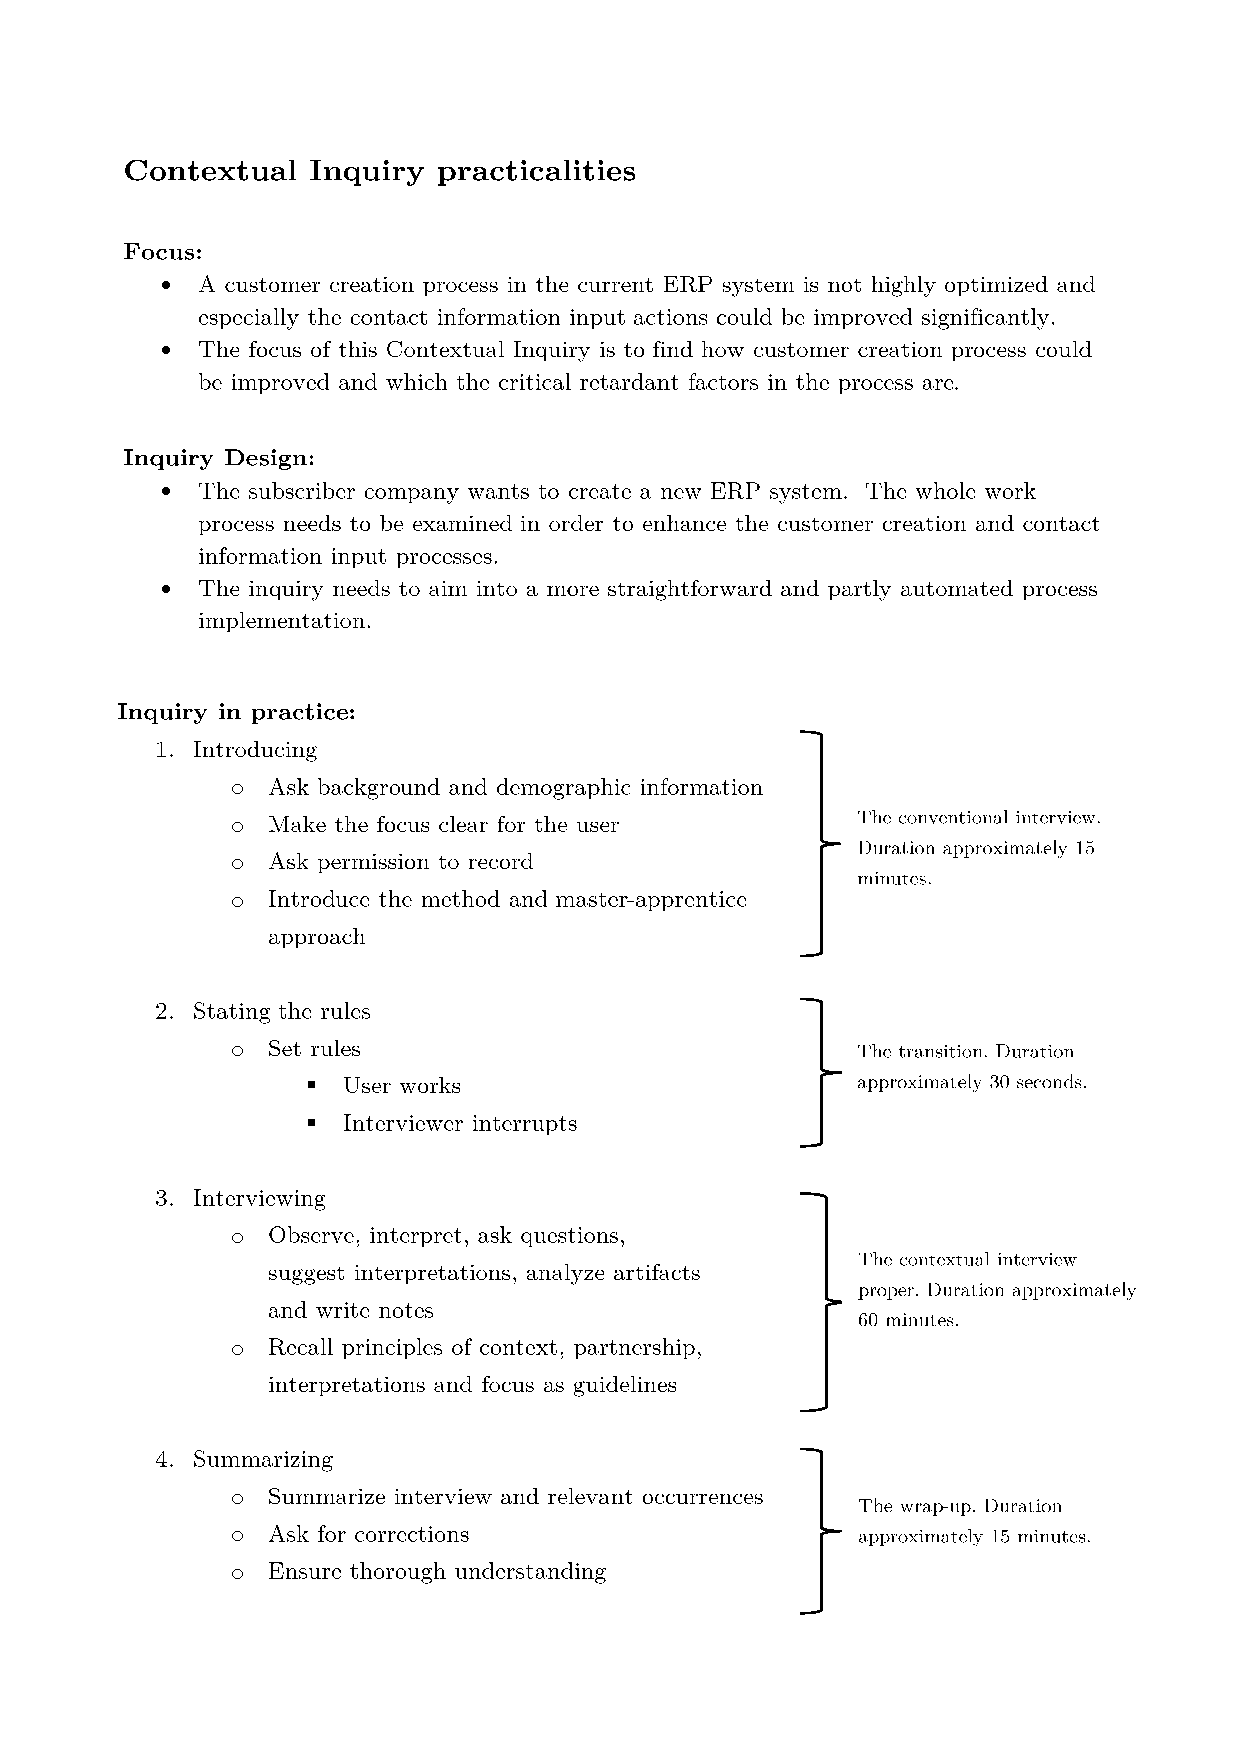
\includepdf[scale=0.85,pages=1,angle=0.0,picturecommand*={%
     \put(95,780){%
         \parbox{\textwidth}{\chapter{Contextual Inquiry: Study plan}\label{app:ciresearch}}
     }}]{./pdfs/ciplan.pdf}



%\includepdf[scale=0.9,pages=4,picturecommand*={%
%     \put(110,770){%
%         \parbox{\textwidth}{\chapter{TEST form}\label{app:susform}}
%     }}]{sus.pdf}


%\includegraphics[scale=0.5,pages={4}]{sus.pdf}

%\includepdf[ pages=4, scale=.7, frame, pagecommand =  \chapter{}]{sus.pdf}
%\chapter{}
%\includegraphics[page=4,width=1.2\textwidth]{sus.pdf}
%\chapter{SUS form}
%\label{chapter:susform}
%\begin{figure}[h]
 %  \centering
   %\begin{tabular}{@{}c@{\vspace{2.5cm}}c@{}}
      % \includegraphics[page=4,width=1.2\textwidth]{sus.pdf} & 

   %\end{tabular}
 %\label{fig:Test}
%\end{figure}



%    \section{APPENDIX A}
%    \label{sec:appendixa}
%This is the first appendix. You could put some test images or verbose data in an
%appendix, if there is too much data to fit in the actual text nicely.

%For now, the Aalto logo variants are shown in Figure~\ref{fig:aaltologo}.

%\begin{figure}
%\begin{center}
%\subfigure[In English]{
\includegraphics[width=.8\textwidth]{aalto-logo-en}}
%\subfigure[Suomeksi]{
\includegraphics[width=.8\textwidth]{aalto-logo-fi}}
%\subfigure[Pä svenska]{
\includegraphics[width=.8\textwidth]{aalto-logo-se}}
%\caption{Aalto logo variants}
%\label{fig:aaltologo}
%\end{center}
%\end{figure}


% End of document!
% ------------------------------------------------------------------
% The LastPage package automatically places a label on the last page.
% That works better than placing a label here manually, because the
% label might not go to the actual last page, if LaTeX needs to place
% floats (that is, figures, tables, and such) to the end of the
% document.
\end{document}
